% EYE - check punctuation in quotes.  Do we put commas and periods on
% the inside or outside?

% Cheezy morse code definitions.
%\newcommand{\mdot}{\raisebox{0.58ex}{\texttt{\makebox[0.33em]{.}}}}
%\newcommand{\mdash}{\makebox[0.5em]{\texttt{-}}}
%\newcommand{\mspace}{\makebox[0.5em]{}}

% To get and use the 'morse' package:
%
%   http://tug.ctan.org/tex-archive/fonts/morse/
%
%   Install morse.sty somewhere.
%
%   Move morse10.mf, morse.alf, morse.def, and morse.num to
%
%     $TEX/texmf.local/fonts/source/public/morse
%
%   and run 'sudo texhash'.
%
% \usepackage{morse}
%
% {\morse SOS}

% Necessary for importing pictures.
%\usepackage{graphicx}

% For clickable hyperlinks.
%\usepackage[colorlinks=true, urlcolor=blue]{hyperref}

% Hyperlinks are written in Roman font (default is typewriter).
\urlstyle{rm}

% Add space between paragraphs, just like chapters 7 and 8 (only) of
% the manual.
% \setlength{\parskip}{1.5ex plus 0.5ex minus 0.5ex}

% Note: only necessary when typeset alone.
%\setcounter{chapter}{8}

%%%%%%%%%%%%%%%%%%%%%%%%%%%%%%%%%%%%%%%%%%%%%%%%%%%%%%%%%%%%%%%%%%%%

%%%%%%%%%%%%%%%%%%%%%%%%%% CHINESE VERSION %%%%%%%%%%%%%%%%%%%%%%%%%
\ifchinese
\chapter{{\\}IFR 转场飞行教程}
\label{IFR Tutorial}

\section{简介}

\begin{figure}[h]
  \begin{center}
    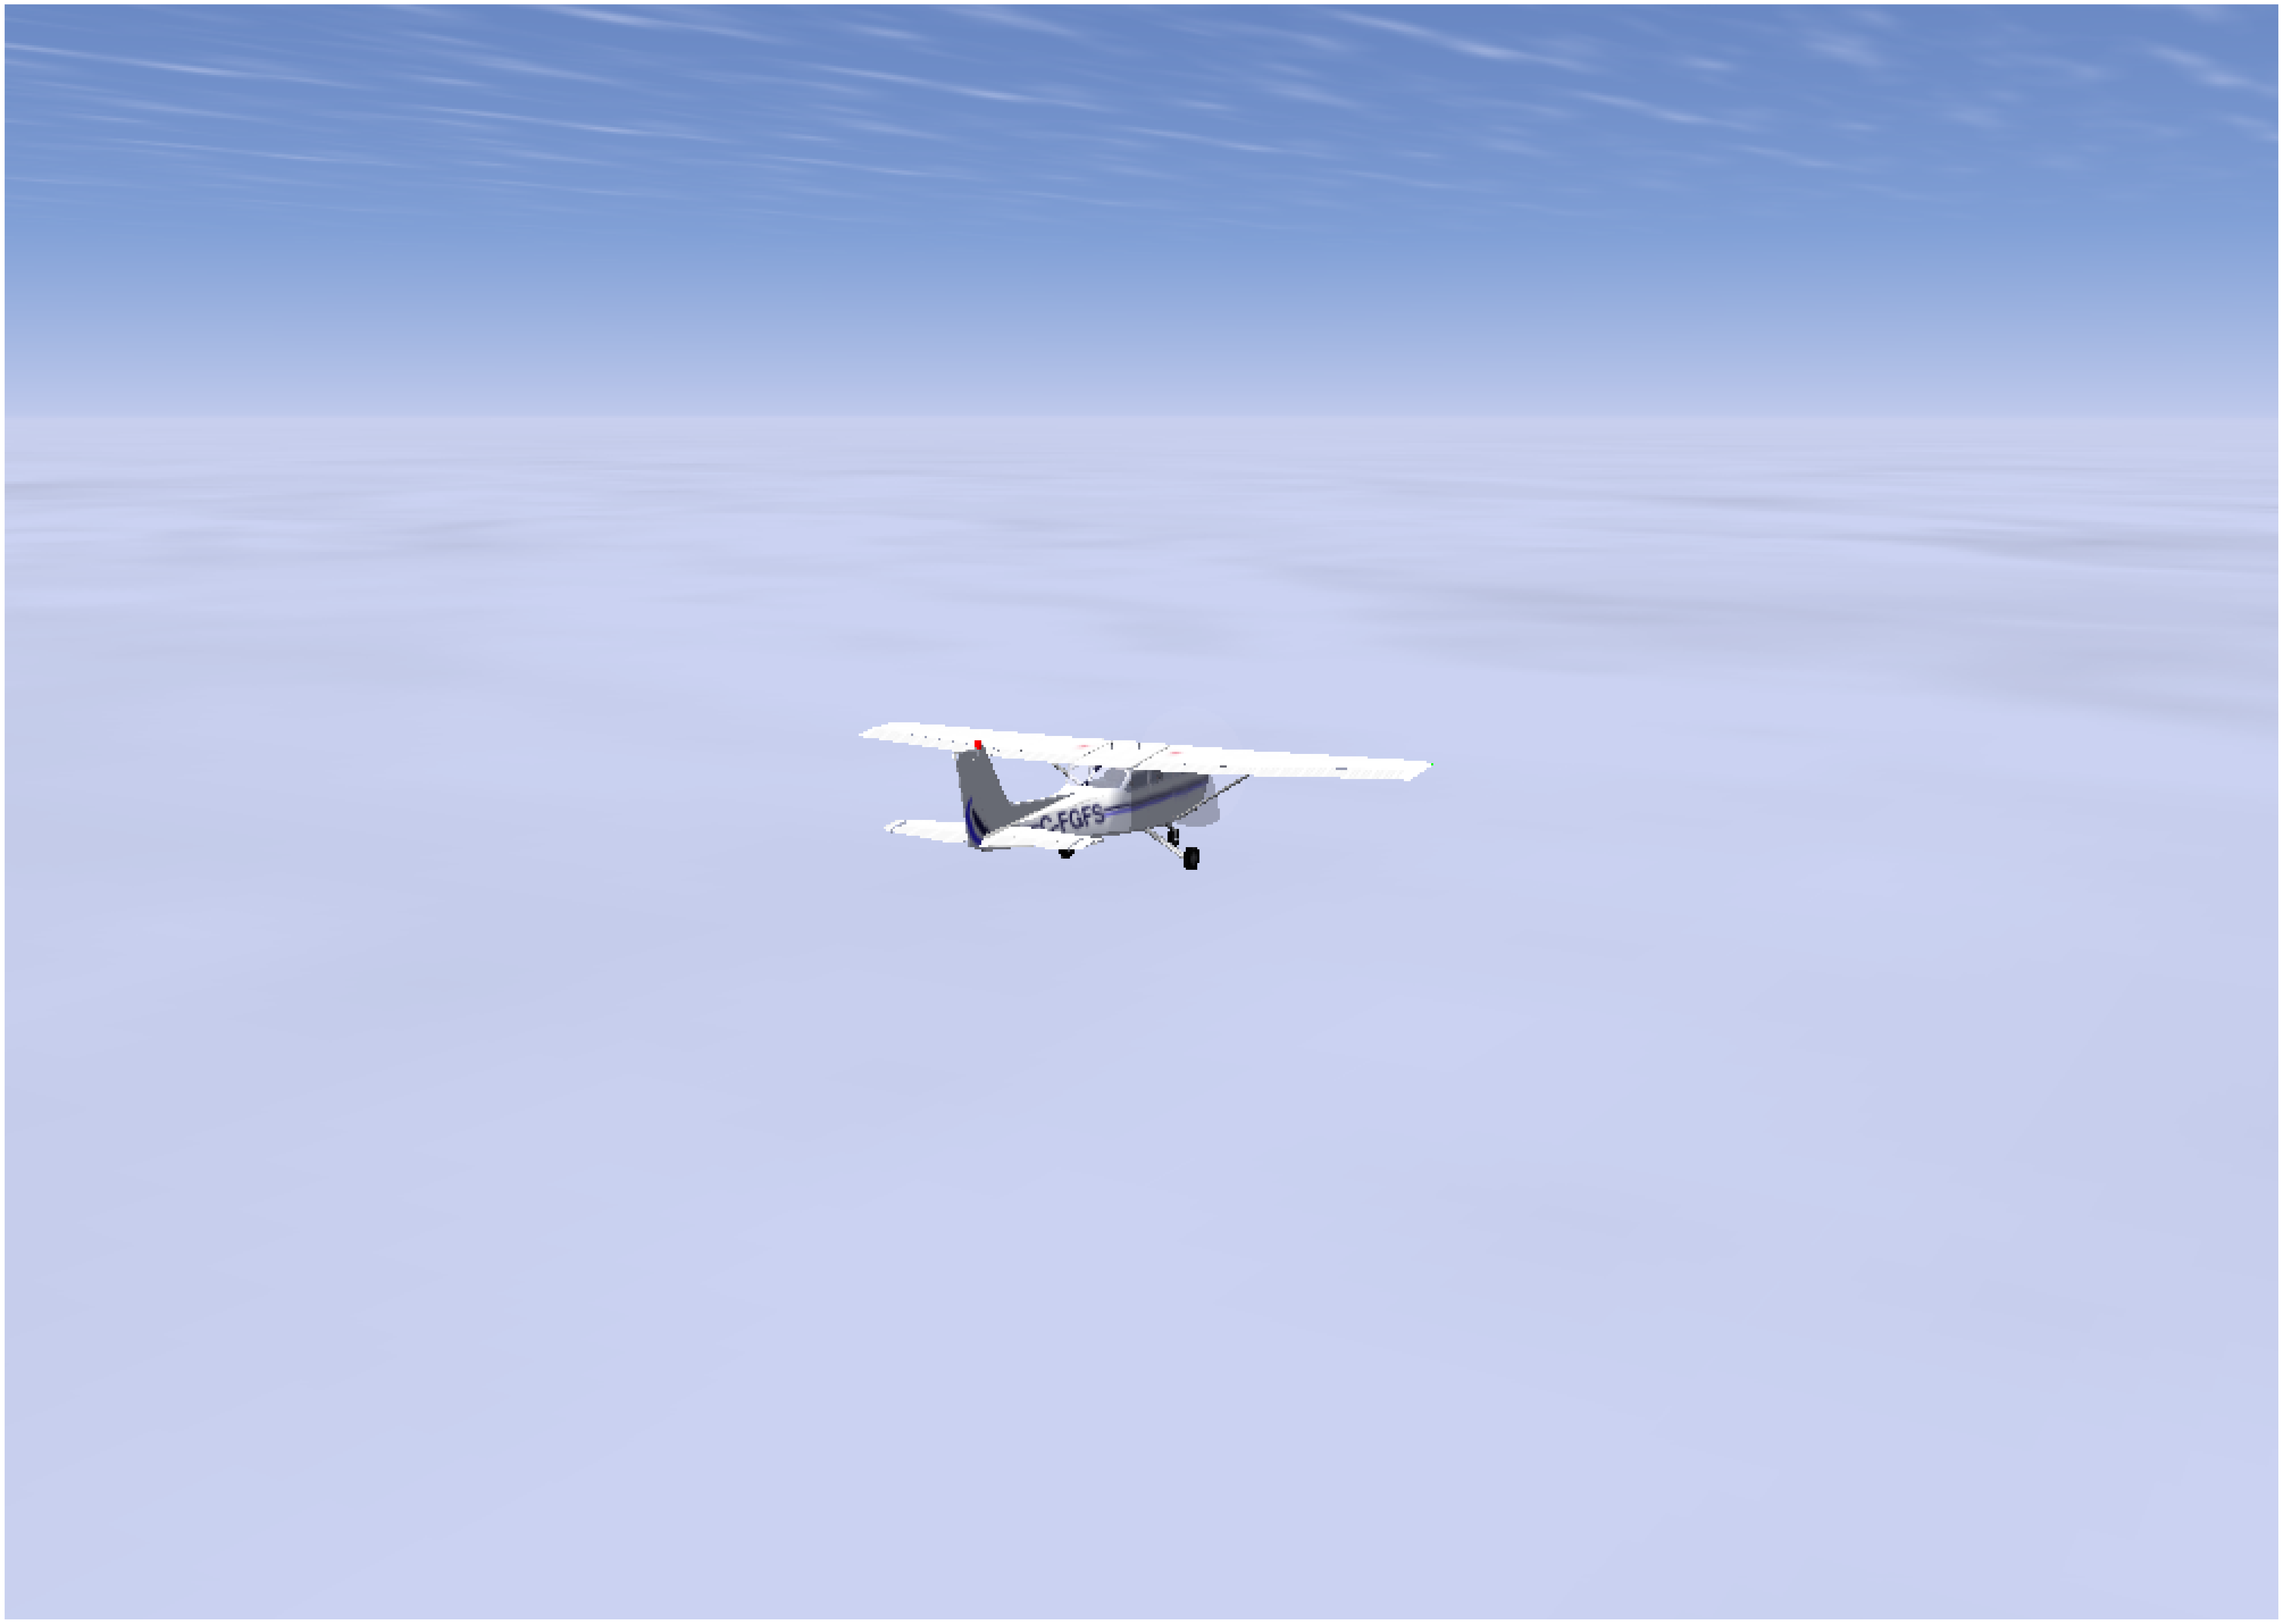
\includegraphics[width=6cm]{img/somewhere}
    \caption{正在从圣安东尼奥大坝飞往利弗莫尔,我猜如此}
    \label{fig:somewhere}
  \end{center}
\end{figure}

之前的转场飞行教程,你已经学会使用 VFR(目视飞行规则)飞行,而在此课程中你将更多学习用仪表飞行 C172P。现在我们将会做一次仪表飞行规则(IFR)下的飞行。此飞行中你将会使用剩下的仪表,学习一点 IFR 飞行,以及很多很多的三字母缩写。

我们将会做同样的飞行,从里德 - 晓岚机场(KRHV)的 31R 跑道飞往利弗摩尔机场(KLVK)的 25R 跑道,只不过这次我们使用 IFR 天气条件:云底高 200 英尺,能见度 800 米。此教程假设你已完成上面的转场飞行教程。

\subsection{免责声明}

此教程不会具体教授 IFR 飞行详情。而仅仅只是帮你建立 IFR 的直观印象,并将之前转场飞行里没有介绍到的仪表细节删除。

我并不是一个飞行员,与之前的教程一样,这些信息大多通过非授权渠道获得。如果你发现错误或误解,请给我发邮件告知:bschack-flightgear -at- usa -dot- net。

此教程已在 FlightGear 3.0 下测试过,其他版本可能与此稍有不同。

\section{起飞之前}

我们需要告诉 FlightGear 我们需要的飞行状况。有很多方式来设置我们需要的天气,这里我们使用全局天气。启动 FlightGear 以后,按 \textbf{\textsf{Environment}} $\Rightarrow$ \textbf{\textsf{Weather}} 启动天气对话框,在 \textbf{\textsf{Weather Conditions}} 里选择 \textbf{\textsf{CAT I minimum}}。

这会降低云层和能见度。不幸的是,这也会造成较大的风。如果你不想面对这些,可以做一些修改:

\begin{itemize}
\item 重新进入 \textbf{\textsf{Weather Conditions}} 并选择
  \textbf{\textsf{Manual input}}
\item 在下面的 METAR 字符串里修改``15015KT''(150 $^\circ$刮来的 15 节风)为 ``15000KT''(风速修改为0)
\end{itemize}

最后按确认键让 FlightGear 准备天气并关闭对话框。

我发现,关闭Atmospheric Light Scattering(大气光散射)可以让渲染更好。打开 \textbf{\textsf{View}} $\Rightarrow$ \textbf{\textsf{Rendering Options}},不要勾选 \textbf{\textsf{Atmospheric light scattering}}。

\begin{figure}
  \begin{center}
    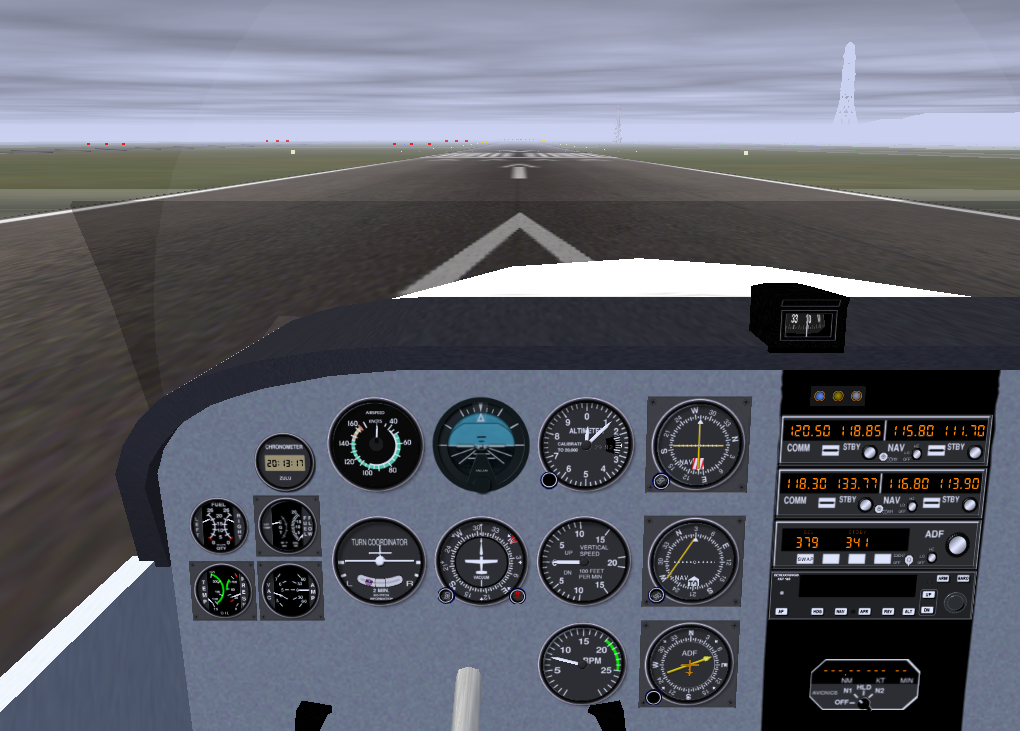
\includegraphics[width=10cm]{img/KRHV}
    \caption{在 KRHV 的 31R 跑道}
    \label{fig:KRHV}
  \end{center}
\end{figure}

\subsection{飞行计划}

如果你从窗户望出去,可能会看到如图 \ref{fig:KRHV} 一样的景致。云层很厚,甚至无法看清跑道尽头。

当无法目视的时候,如何从 A 点到 B 点呢?多年来先驱已经总结了多种方法,各有优缺点。我们的教程将会使用塞斯纳 C172P 上所有的导航仪表,尝试各种可能性。

我们的整条航线,以及用到的导航设施都在图 \ref{fig:sectional_labelled} 里标示出来了。绿色是我们的航路,导航设施用蓝色和红色标出。航路有一点疯狂——也许你会想我们如果多使用这些设备而不是靠大脑方向感,就不会迷航了——方法很疯狂。如其在这里将这些问题都解释清楚,不如下面我慢慢道来。

\begin{figure}
  \begin{center}
    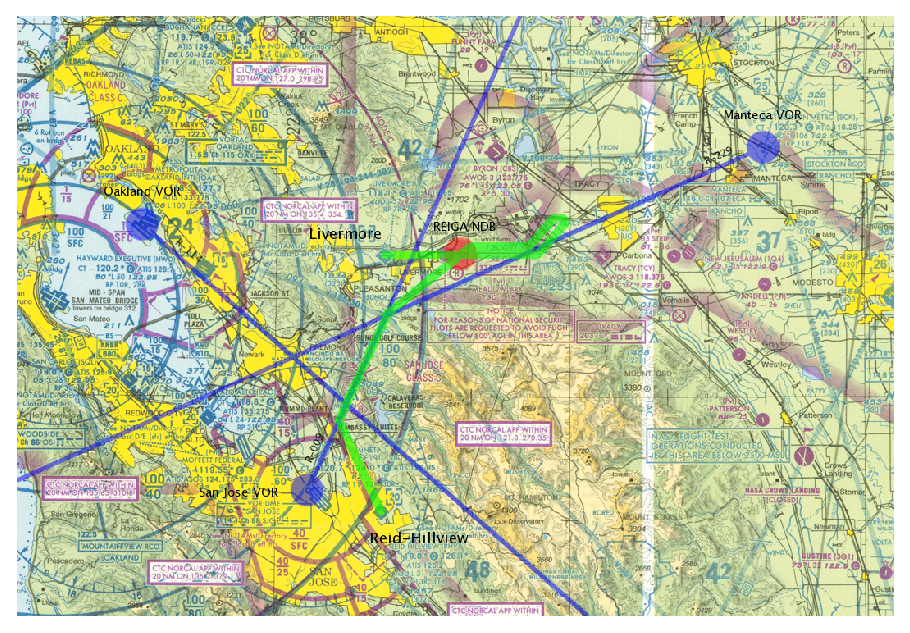
\includegraphics[width=20cm, angle=-90]{img/sectional_labelled}
    \caption{绿色:我们的航路,蓝色:VOR 及其径向线,红色:NDB}
    \label{fig:sectional_labelled}
  \end{center}
\end{figure}

\subsection{VHF 全向信标}

首先我们来使用 VOR\footnote{关于 VOR 的更多详情可参见维基百科 \url{http://en.wikipedia.org/wiki/VHF_omnidirectional_range}}(VHF(Very High Frequency) Omnidirectional Range,甚高频全向信标)导航,它会将我们带到利弗摩尔南方 5 海里左右的位置。

区域航图里用翠绿色有罗盘标记的大圆圈住 VOR 信标台。我已经在图中用蓝色标记出来了。从图 \ref{fig:sectional_labelled} 里可以看到里德 - 晓岚机场与一个 VOR 信标台(San Jose\footnote{San Jose 是美国地名圣何塞,下文中的 Oakland 也是地名奥克兰。此手册中所有的 VOR、NDB、ILS 和导航点的名称,均保持原文不做翻译,以方便读者在航图中查询和理解,下同/。——译者注})很近,在圆圈的中心有一个翠绿色的方框,可以看到信标台的信息。根据这些信息,可以看到这是个 VOR-DME 信标台(稍后解释何为 DME),名字是 San Jose,频率是 114.1 MHz(或者 88 频道,同一个事情的另一种说法),其识别码或“ident”是 SJC(莫尔斯码是 \mdot\mdot\mdot\mspace\mdot\mdash\mdash\mdash\mspace \mdash\mdot\mdash\mdot)

要调到 VOR 信标台,我们需要使用两台 NAV 接收机中的一台。也就是与 COMM 捆绑在一起的接收机(可参考图 \ref{fig:panel})。同时我们用对应的 VOR 仪表指针。在此例子中我们会选择 NAV1 接收机(对应的是 VOR1 仪表指针),当然也可以用 NAV2。调节频率之前,先来检查 VOR1 仪表。其应该如图 \ref{fig:VOR1} 中左侧的 VOR1。最重要的是红色的“NAV”指示器。这表示没有收到 VOR 信号,因此我们不能相信此仪表。

\begin{figure}
  \begin{center}
    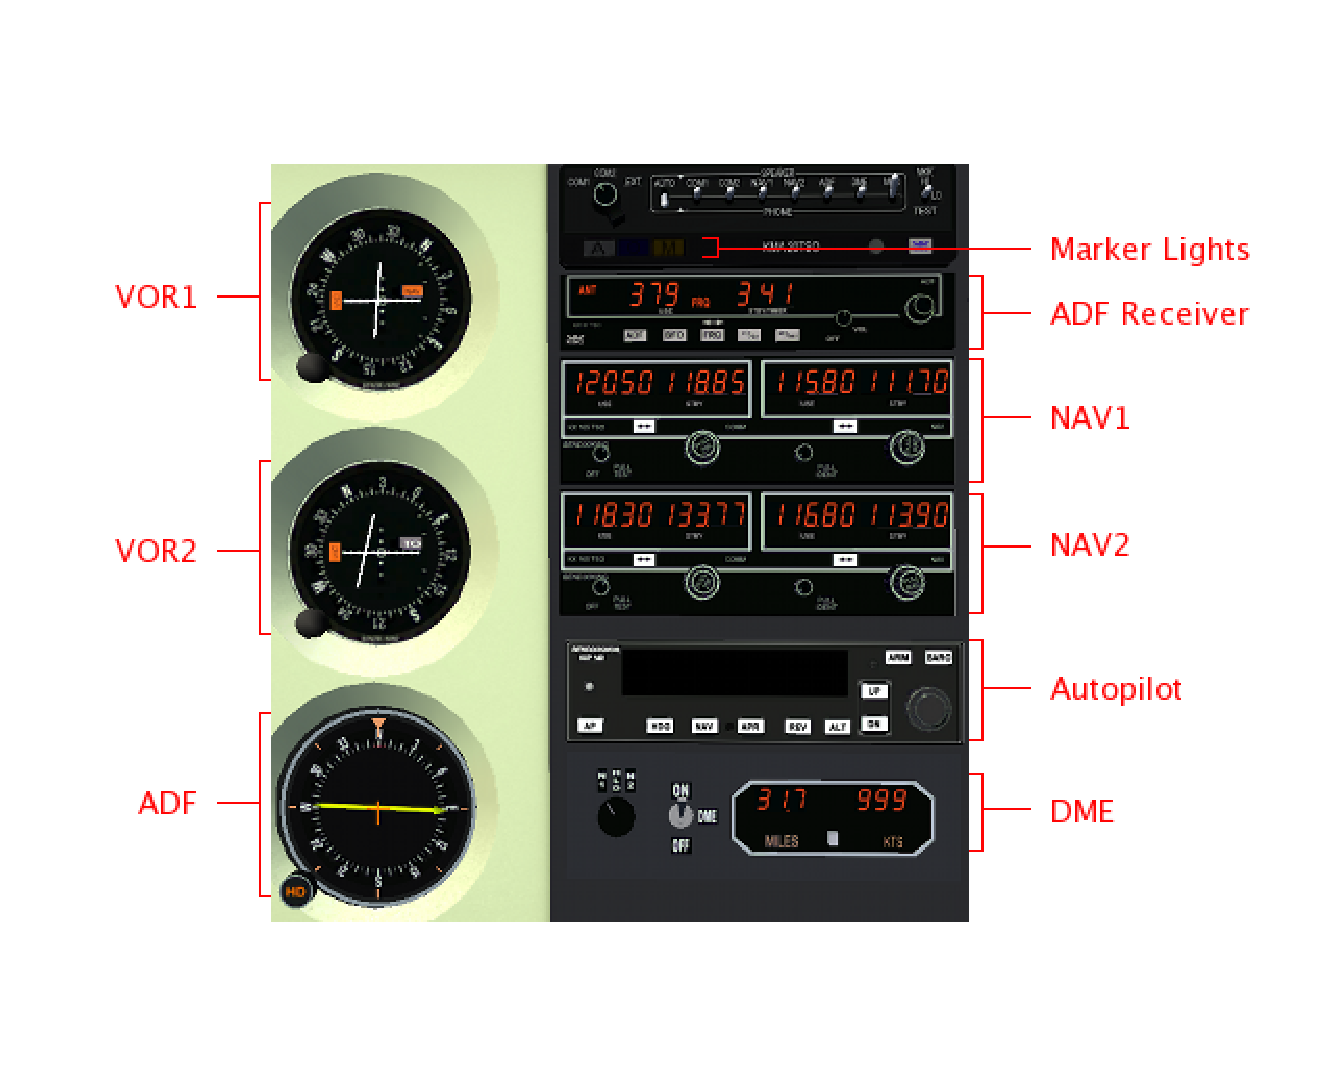
\includegraphics[width=12cm]{img/panel_labelled}
    \caption{IFR 导航仪表}
    \label{fig:panel}
  \end{center}
\end{figure}

NAV 接收机有一个活动频率和一个备用频率,还有一个调频旋钮,与 COMM 接收机类似\footnote{操作 COMM 接收机的教程,已经在上一章的教程里介绍过。}调节其频率到 114.1,并按 SWAP 交换按钮\marginpar{\textsf{NAV1 $\Rightarrow$ 114.1}\footnotemark}\footnotetext{所有重要操作都会放在页边,避免与正文冗长的文字放在一起,更利于飞行参考}。如果你观察 VOR1,你会注意到红色的“NAV”消失了,取而代之的是“TO”标识\footnote{VOR1/2 的 TO/FROM 指示器,“TO”会翻译为“向台”,而“FROM”会翻译为”背台“。——译者注},正如图 \ref{fig:VOR1} 左侧所示。这表示我们收到了信号,然而这是不是正确呢?如果我们恰好设置了错误的频率呢?

\begin{figure}
  \begin{minipage}[b]{0.5\linewidth}
    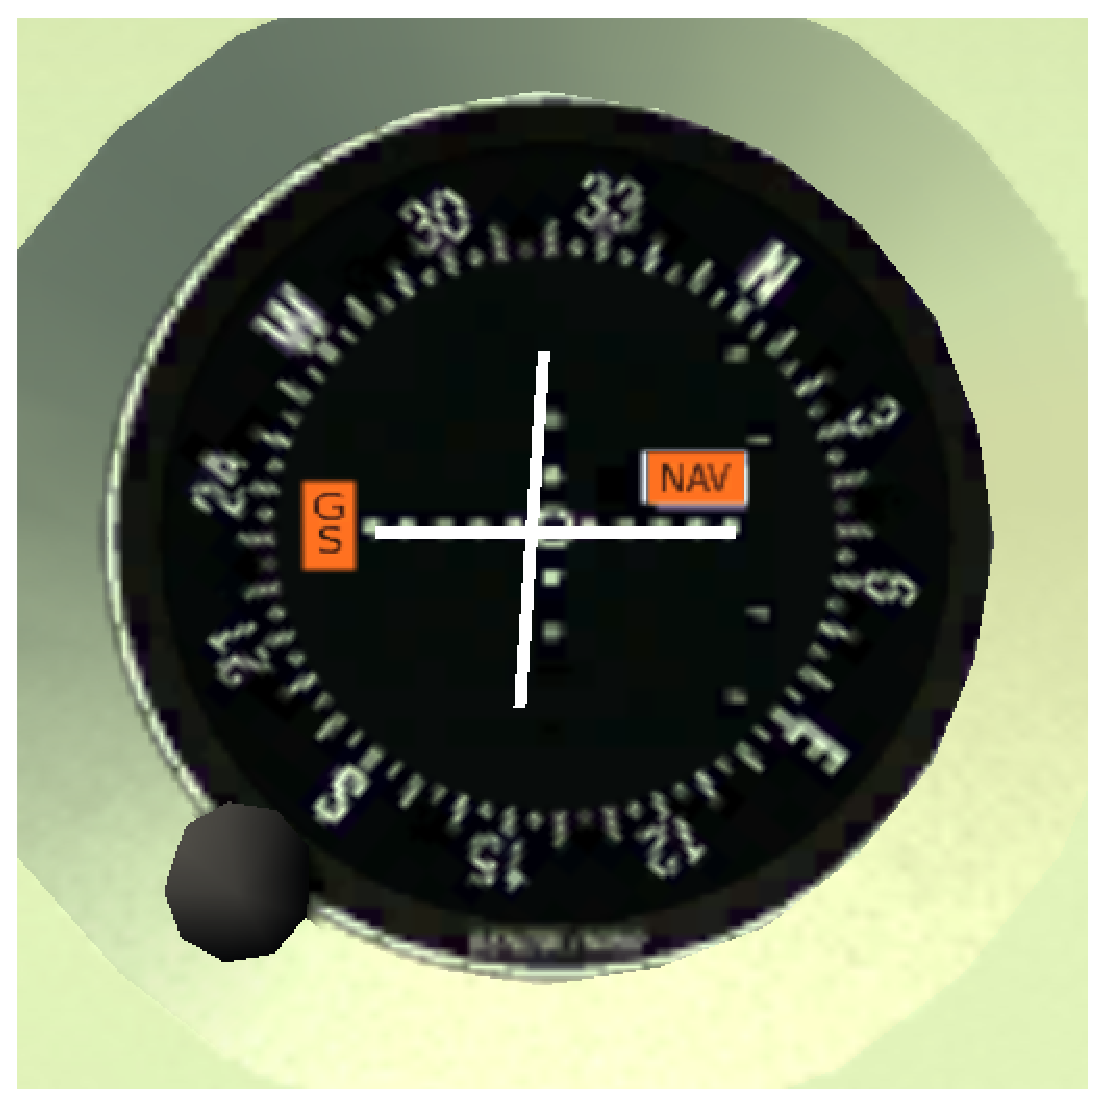
\includegraphics[width=6cm]{img/VOR1_before}
  \end{minipage}
  \hspace{0.5cm}
  \begin{minipage}[b]{0.5\linewidth}
    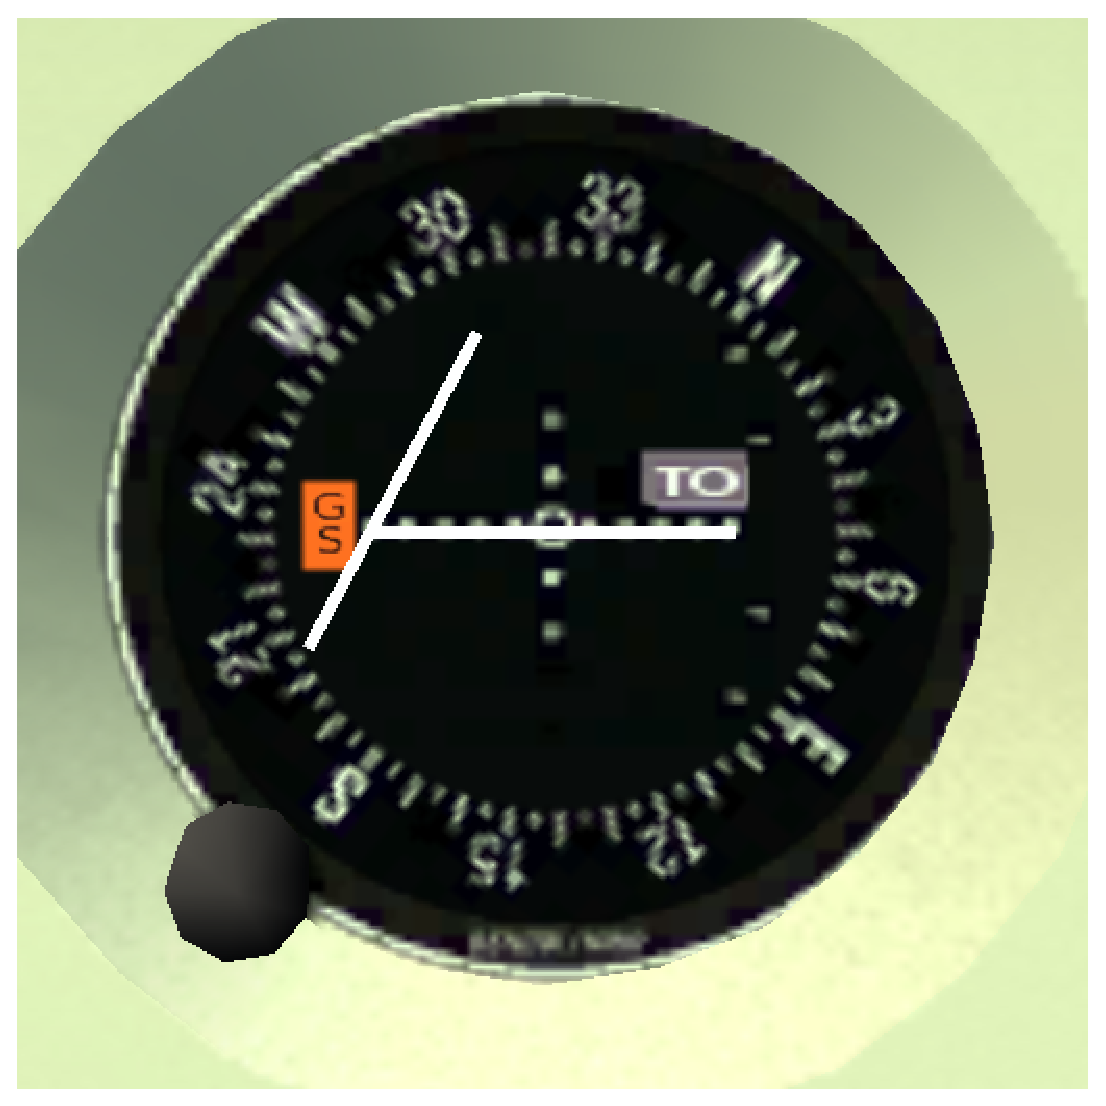
\includegraphics[width=6cm]{img/VOR1_after}
  \end{minipage}
  \caption{VOR1,调节频率之前和之后}
  \label{fig:VOR1}
\end{figure}

为了确认我们调到了正确的 VOR 信标台,我们可以听其识别码。如果你听不到,可能是不符合航图,此时不要相信指针。目前为止,也许你还没有听到任何声音。为什么呢?检查音频面板(参考图 \ref{fig:panel})。你会注意到有很多开关控制这些设备,NAV1 也在其中。将开关向上拨(或向下——无所谓),你能听到莫尔斯码 \mdot\mdot\mdot\mspace
\mdot\mdash\mdash\mdash\mspace \mdash\mdot\mdash\mdot\footnote{若还不能听到,检查 NAV1 接收机的音量。若还不行,打开 \textbf{\textsf{File}} $\Rightarrow$ \textbf{\textsf{Sound Configuration}} 并设置声音。检查你电脑的音量,外接音箱的音量。如果依旧不行,检查听觉}。若已经厌倦了听莫尔斯码,可以将开关拨回中间。

回到 VOR1。左下方还有一个旋钮,叫做 OBS(OmniBearing Selector,航道选择旋钮)。正如名字所说,此旋钮用来选择航道。如果你旋转这个旋钮,你能看到垂直的指针在动,这个指针称之为 CDI(Course Deviation Indicator,航道偏离指示器)\footnote{水平的指针用于 ILS 降落,稍后会解释}。尝试让指针维持在中间,此时小三角应该指在 277 左右。这个数字配合 TO 指示表示:“正在 \emph{277$^\circ$} 航向上\emph{向台}飞行”。

好了,根据我们的航路,我们不会这么\emph{向台}飞行,我们会截获图上蓝色的那条 009$^\circ$ 径向线,\emph{背台}(FROM)飞行。如何做呢?非常简单,设置 OBS 到 009 \marginpar{\textsf{VOR1 OBS $\Rightarrow$ 009}}。当穿过径向线时,指针会回中,同时指示器会变成 FROM。这意味着“正在沿 009$^\circ$ 航向背台飞行”,这正是我们想要的,因此在截获径向线时我们转向 009$^\circ$。

起飞前最后一件事,设置方向陀螺仪的航向游标到当前航向,大概 310$^\circ$。 \marginpar{\textsf{航向游标 $\Rightarrow$ 310}}.

\subsection{我们要飞多高?}

设置好天气以后,气压值就不再是标准的“29.92”了。我们需要直到正确的高度表拨正值,否则高度表会设置错误高度。在起飞时也许不严重,但在云中下降时,却有\emph{巨大}的不同(你也许会说这是“可控飞行撞地”\footnote{CFIT,Controlled flight into terrain})。

正如上一章的短途转场飞行教程所说,我们可以通过 ATIS 来获取当前气压值。进入 \textbf{\textsf{AI}} $\Rightarrow$ \textbf{\textsf{ATC Services in Range}} 并选择我们的起飞机场,搜索 ATIS 频率(应该是 125.20 MHz)。将 COMM1 或 COMM2 设置在这个频率(记得在音频面板上打开相应的声音),收听机场通播,并注意调节高度表拨正值。

我们会使用自动驾驶仪(如图 \ref{fig:panel} 和 \ref{fig:ap_vs})来稳定高度(稍后介绍)。因此自动驾驶也需要知道大气压。按自动驾驶仪上的 BARO 按钮,你会看到“29.92”显示出来了,这就是自动驾驶仪内部的大气压值。在 29.92 消失之前(大概 3 秒),转动小旋钮改变其值。

\section{起飞}

好了,起飞以后暂时保持航向 310$^\circ$。\marginpar{\textsf{起飞;沿跑道航向爬升}},建立正上升率。我们计划爬升到 4000 英尺,现在只有唯一的一个问题——我们面前这些丑陋的云在挡路。

\section{在空中}

如果这是你第一次尝试 IFR 飞行,你也许会发现几乎不可能在云中飞行,因为缺少目视参参考。也许你会说“没关系,只要保持稳定就可以”。有时候,你会发现指针疯狂旋转,飞机也会进入螺旋,上上下下或失速,也可能各种运动复合在一起。

我们需要练习在没有目视参考的情况下飞行,这是在学习 IFR 时必须掌握的技能。而现在,我们使用自动驾驶来让飞行简单一些。

\subsection{自动驾驶 I}

当我们建立正上升率并开始爬升时,按自动驾驶仪上的 AP 按钮启动自动驾驶。你会看到“ROL”显示在左侧,表示“滚转模式”——会保持机翼水平,中间会显示“VS”,表示“垂直速率模式”——会保持恒定的升降速率。右侧会看到在 AP 启动\emph{瞬时}显示的升降率。初始,此值就是自动驾驶启动时的升降速率。比如图 \ref{fig:ap_vs},自动驾驶将垂直速率设为 300 fpm。

\begin{figure}
  \begin{center}
    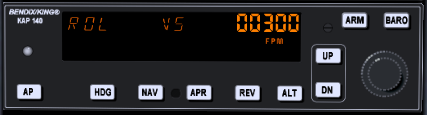
\includegraphics[width=7cm]{img/ap_vs}
    \caption{启动之后的自动驾驶}
    \label{fig:ap_vs}
  \end{center}
\end{figure}

当你启动自动驾驶以后,请仔细确认此升降率。有时自动驾驶会进入很怪异的状态,比如 1800 fps。我们的小塞斯纳可无法承受,很可能会进入失速状态。这可能是一个 bug,为了保险起见,你需要防止设备出问题。你需要不断交叉检查设备,并随时应对可能的问题。

我们需要垂直遂率在 500 到 700 fpm。按 UP 和 DN 按钮,来调节垂直速率的值。还要考虑到空速,我们需要合适的爬升率。

最后,当爬升率建立以后,按航向按钮(HDG)\marginpar{\textsf{启动自动驾驶;设置垂直速率;启用航向模式}}。此时“ROL”会变成“HDG”,因为你刚刚已经将航向游标设置在了跑道航向,所以此时飞机不会有大的转弯。

\subsection{MISON 交汇点}

此时大概距离我们要截获的 009 径向线 8 海里的位置,因此我们还有一些时间。因为没有可观察的地面景物,如图 \ref{fig:murk},我们需要准备下一阶段飞行。

\begin{figure}
  \begin{center}
    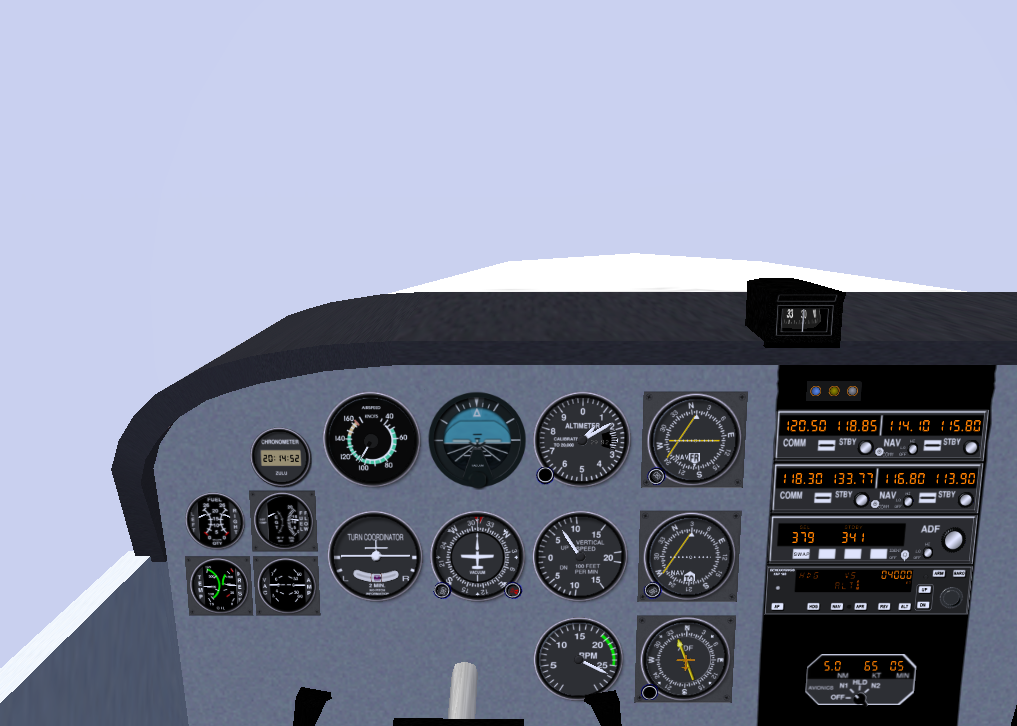
\includegraphics[width=6cm]{img/murk}
    \caption{典型 IFR 场景}
    \label{fig:murk}
  \end{center}
\end{figure}

如果你看一下我们的航路,截获 009 径向线并向北,我们会经过一个角 MISON 的交汇点(如同 \ref{fig:Oakland} 中更细致的图示,MISON 在右下能找到)。在 MISON 上面可以看到交叉的十字,表示 MISON 是航路交汇点。实际上我们会飞过 MISON 的东侧,但径向线是西北到东南的穿过 MISON,我们对此没兴趣。我们只是用其来监视飞行过程。

\begin{figure}
  \begin{center}
    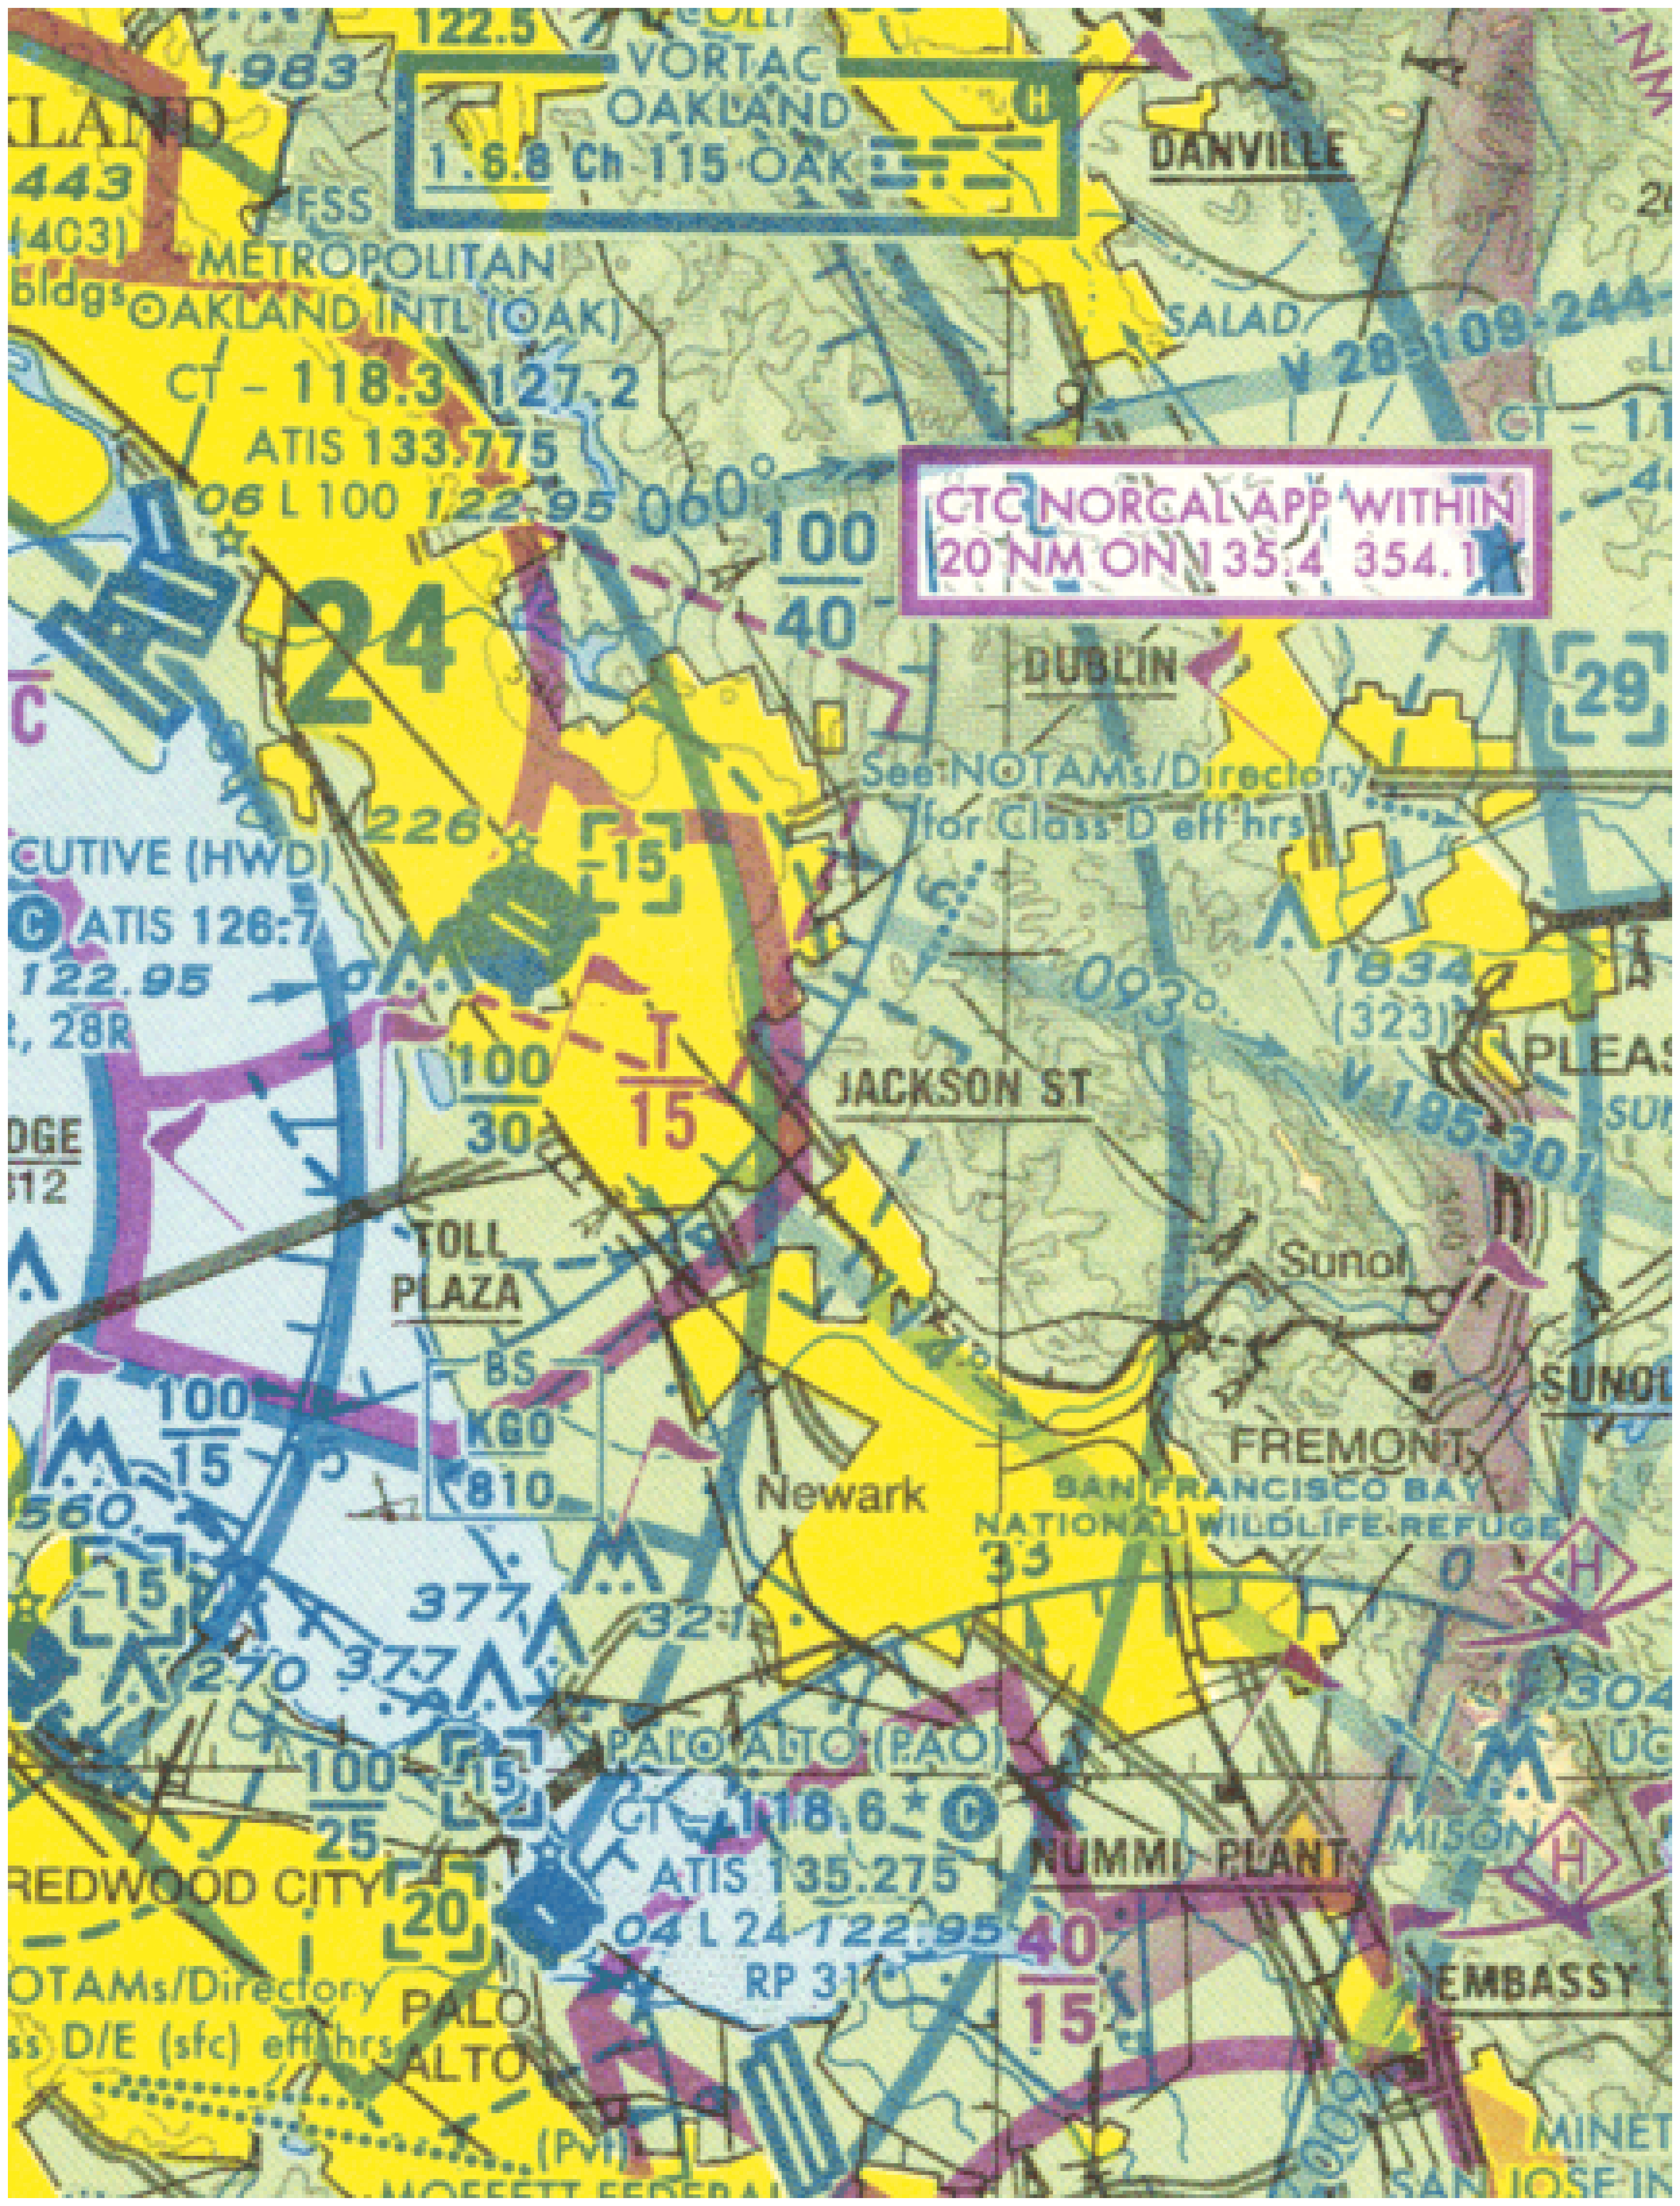
\includegraphics[width=10cm]{img/Oakland}
    \caption{Oakland VOR 及 114 径向线穿过 MISON 交汇点}
    \label{fig:Oakland}
  \end{center}
\end{figure}

我们只需要沿着 009 径向线背向 San Jose 台飞行,直到我们需要转弯的时候。但这个交汇点很重要:第一,可以检查我们到哪了。第二确认我们想象的飞到哪里。如果我们一直飞阿飞,没有穿越径向线,就需要警告自己了。

观察区域航图,我们可以看到径向线是背向 Oakland VORTAC(VOR TACAN,TACAN 表示 Tactical Air Navigation,战术空中导航) 114 度。Oakland 的频率是 116.8,其识别码是 OAK(\mdash\mdash\mdash\mspace \mdot\mdash\mspace \mdash\mdot\mdash)。我们需要将 NAV2 设置在 Oakland,现在就设置吧\marginpar{\textsf{NAV2 $\Rightarrow$ 116.8}}。同时打开音频面板上的 NAV2 确认收到了正确的识别码。

我们需要调节 OBS,告诉 VOR2 我们关注哪条径向线。设置 OBS 到 114\marginpar{\textsf{VOR2 OBS $\Rightarrow$
    114}} \footnote{如果你对手动调节频率感觉厌烦,可以用 \textbf{\textsf{Equipment}} $\Rightarrow$ \textbf{\textsf{Radio Settings}} 对话框}。你可以猜测一下,当我们穿过 114 径向线的时候,VOR 上会指示 TO 还是 FROM。也可以猜测指针会从左向右运动,还是从右向左运动。

最后要说,依照我们的目的,无所谓是什么径向线,可以是 113,115,或者 100 或者 90,之所以选 114 是因为恰好图上标注出来了,这样就不用自己画了。

\subsection{自动驾驶 II}

在我们继续飞往截获 009 径向线的路上,让我们在近距离了解一下自动驾驶。首先,如果你没有使用调整片的习惯,你会看到自动驾驶仪上经常会有闪烁的“PT”标志。这是自动驾驶仪在提醒你用调整片调整一下飞机。我倾向于忽略这个,因为用鼠标飞行时,不调整反而更好。而那些使用游戏杆或驾驶盘的朋友,也许多多使用调整片会避免出现这个提醒。

同时,右侧还有一个大旋钮,也就是高度选择旋钮,可以用这个旋钮来调节目标高度。我们需要用到它,调节旋钮直到达到目标巡航高度,4000 英尺,显示在右侧。当你调节旋钮的时候,“ALT ARM”会显示在自动驾驶仪上(如图 \ref{fig:ap_alt} 所示),这表示你已经修改了目标高度\marginpar{\textsf{设置自动驾驶仪目标高度 4000}}。自动驾驶仪会保持当前上升率直到这个目标高度,之后会改平飞并从垂直速度模式(VS)变成高度保持模式(ALT)。在高度保持模式,它会保持在一个固定高度(比如此例中的 4000 英尺)\footnote{当然,你也不一定要如此,你可以叮着高度表,当到达 4000 英尺时,将上升率设置为 0,然后按 ALT 按钮进入高度保持模式。之所以多介绍一个旋钮,也是为了揭秘更多自动驾驶仪相关的内容}。当你距离目标高度还有 1000 英尺,也就是到达 3000 英尺时,会听到 5 声蜂鸣报警音表示高度保持模式进入预位状态。

\begin{figure}
  \begin{center}
    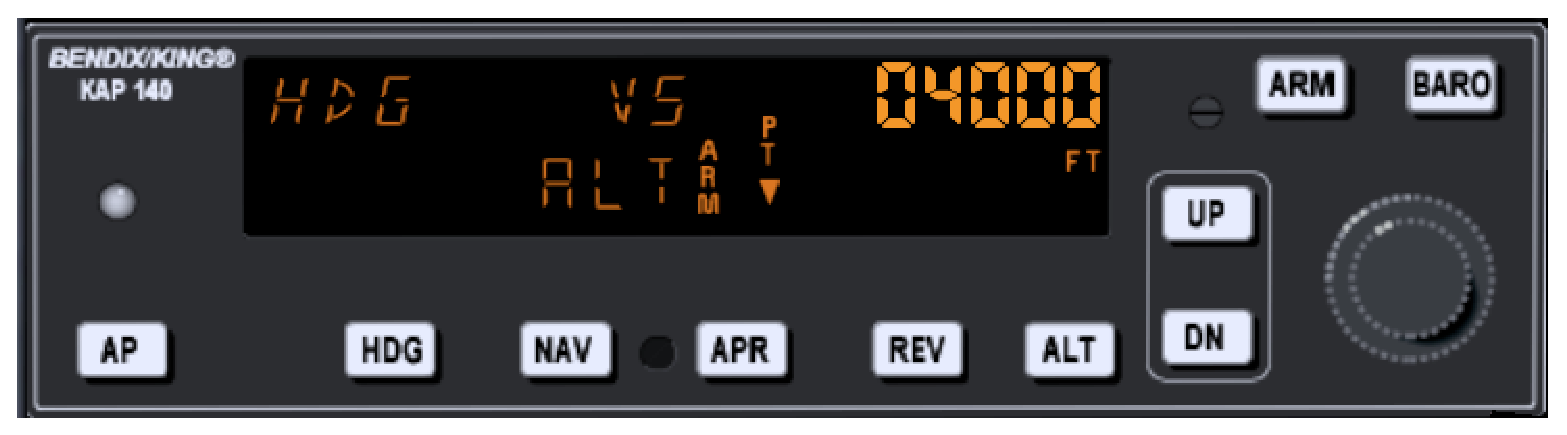
\includegraphics[width=7cm]{img/ap_alt}
    \caption{高度保持模式进入预位状态时的自动驾驶仪}
    \label{fig:ap_alt}
  \end{center}
\end{figure}

注意,自动驾驶不会调节油门,因此当飞机改平飞时,速度会增加。你需要适时修正油门符合巡航需求。

\subsection{保持航道}

你可能会截获到 009 径向线(也就是 VOR1 的 CDI 指针在中间位置)。然后转向 009 \marginpar{\textsf{当 VOR1 截获后转向 009$^\circ$}}。若使用自动驾驶仪的话,你可以通过修改方向陀螺仪上的航向游标。

除非你做的足够好且幸运,否则指针也许不会回中。我们需要调整一下航道。CDI 指针(VOR 上的竖直指针)会告诉我们飞向哪里。如果它在左侧,表示径向线在我们的左侧,因此我们要向左飞。反之亦然\footnote{原文这里缺少一个前提条件,当向台飞行时(TO)符合这个规律,而背台飞行(FROM)时指针和飞机运动是相反的,即指针向左偏转时,我们需要向右飞行以截获径向线。读者可在 FlightGear 里亲自实验并领会。——译者注}。

理论上很简单,然而在实践中你会发现很难保持指针一直在中间,会被风吹离径向线。关键是:指针的\emph{位置}告诉我们\emph{在哪里},而指针\emph{运动的方向}告诉我们要\emph{如何做}。

我来解释一下,如果指针在我们的左侧,那么无疑径向线也在左侧\footnote{除非你向相反方向飞行,那就是另一种情况了。}。如果指针正在向我们\emph{移动},表示你正在或早或晚会穿过径向线,所以我们需要更快的进入径向线或者等待指针回中。另一方面,如果指针正在\emph{远离}我们,我们需要组织这种趋势,逆转它的运动。

注意,刚开始我们很难猜测需要转多少。可先尝试转 10$^\circ$,如果指针运动太快,我们就改成 5$^\circ$(或反向 5$^\circ$)。如果另一种情况,指针移动太慢,我们就加大到 20$^\circ$(另外增加 10$^\circ$),然后看看会发生什么。

\subsection{更多的交叉检查}

经常交叉检查飞机的位置是个好习惯。与 Oakland 114 径向线的交汇点就要到了\marginpar{\textsf{穿过 OAK 114 径向线}}。前方就是 SUNOL 交汇点。如果你仔细看,5 条径向线交汇在此,因此我们要选择使用哪条径向线。因为之后会非常有用,我们将会使用右上的那条,它是 Mantech VORTAC 的 229 径向线,频率 116.0 MHz,识别码 ECA(\mdot\mspace \mdash\mdot\mdash\mdot\mspace \mdot\mdash)。

你应该已经知道该如何做了:调节 NVA2 到 116.0,设置 OBS 到 229,并检查确认信标台识别码\marginpar{\textsf{NAV2
    $\Rightarrow$ 116.0\\VOR2 OBS $\Rightarrow$ 229}}。

同时,让我们介绍仪表板上的另一个功能,用来交叉检查 SUNOL 交汇点。一些 VOR 信标台有测距的功能,也就是 DME\footnote{详情可参考\url{http://en.wikipedia.org/wiki/Distance_Measuring_Equipment}。}(Distance Measuring Equipment,测距装置)。比如 San Jose 就有(还记得它是 VOR-DME 信标台),而 Oakland 和 Manteca 也有(VORTAC 具备 DME 的能力)。

使用 DME,你可以知道我们飞了多远,距 VOR 信标台的直线距离。在我们的场景中,DME 不重要,但我们依旧会使用,学习它怎么工作,也确认我们的位置。

DME 仪表就在自动驾驶的下方\footnote{有些是在自动驾驶仪的上方。——译者注}(可参考图 \ref{fig:panel})。确保已经打开它,左边的开关旋钮一般是在 N1 位,而“N1”则表示“收听 NAV1”。因为现在 NAV1 是 San Jose 频率,这样就告诉我们距 San Jose VOR-DME 信标台的距离。我们把旋钮转到 N2\marginpar{\textsf{DME $\Rightarrow$ N2}},这样会告诉我们距 Manteca VOR 的距离。

DME 会先是三样东西:距离信标台的海里数,飞向或远离信标台运动的速度,以及按此速度飞向信标台所需时间。注意此处的距离是飞机到信标台的直线距离(也就是所谓“斜距”),而不是地面距离。同样速度也是相对信标台的速度,因此除非你是向台或背台直飞,否则这个速度会略低于你真实的地速。比如,从 San Jose 背台飞行,它就在我们后方,会稍快于我们向 Menteca 信标台的速度,因为它在我们右侧。

如果我们要搜索有关 SUNOL 交汇点的信息\footnote{比如使用 \url{http://www.airnav.com/airspace/fix/SUNOL}.},会告诉我们它在 ECA 信标台 229.00 径向线 33.35 海里的位置(也就是``ECAr229.00/33.35''表示的含义)。

现在我们有两种方法确认 SUNOL 交汇点:VOR2 指针会回中,DME 的读数是 33.4 左右。注意,DME 不会提供精确修正,因为 Manteca 信标台的测距有个角度\footnote{因为这个角度很小,所以常常将 DME 测得的距离等同于地面距离。吐个槽,原文这里最好有个图。——译者注}。

你也许会问 DME 上 HLD 的含义(也就是 N1 和 N2 之间)。这表示“Hold”(保持),意思是“不管 NAV1 和 NAV2 如何调节,DME 都保持当前频率”。比如如果我们从 N2 调到 HLD,DME 依旧会显示我们到 Manteca 的距离,即使我们重新调节 NAV2,DME 始终会保持在 Manteca。这非常有用,相当于 DME 变成了第三台独立的接收机,IFR 飞行时两台接收机看上去不够用。

\section{准备下降}

我们正在靠近 SUNOL,沿着 San Jose 的 009 径向线,关注着 DME 上的位置。在 SUNOL 点,我们距离利弗摩尔就不到 5 海里了,也就是云层下方的某处。也许我们降到 700 英尺左右(利弗摩尔标高 400 英尺,而云底高 750 英尺)并稍稍向北就能到了吧?我的朋友也许一场灾难即将降临,你会懂的。

\subsection{仪表进近程序}

正如上一章的教程所述,当我们飞 VFR 的时候,你不能让飞机直接向最近的跑道落地。你需要飞到起落航线中,这会帮你对准跑道,并避免与其他飞机相撞,这是一件好事。

IFR 与此类似,也有流程可循。事实上,确实有\emph{程序}\footnote{此处的“程序”是为“Procedure”一词的中文翻译,在民航领域中,一般带有流程性的内容称为“程序”,不要与计算机相关的“程序”混淆。——译者注}可用。因为 IFR 降落的复杂性,没有一个适用于所有机场的固定程序。你需要根据特定的机场检查相应的程序。事实上,你需要检查特定机场、跑道和导航设备。

我们的机场是利弗摩尔(Livermore,KLVK)。让我们搜索它的信息。前往 \url{http://www.airnav.com/airport/KLVK}\footnote{此网站只提供美国境内的机场和导航设备信息。——译者注}。在靠近底部的位置,我们可以看到 IAPs(Instrument Approach Procedures,仪表进近程序)。表里有两个 25R 跑道的仪表进近程序,一个是 ILS(Instrument Landing System,仪表着陆系统) 进近,另一个是 GPS(Global Positioning System,全球定位系统) 进近。因为我们没有安装 GPS 设备,但我们可以 ILS 进近(稍后介绍),因此我们就选这个了。

虽然利弗摩尔只有两个仪表进近程序,而大型机场则有很多。如果看一下附近的旧金山机场,你可以看到\empth{大量}的程序,有 ILS 程序、GPS 程序、LDA 程序、VOR 程序等等,学习 IFR 飞行,你会学到所有这些程序。

回到利弗摩尔,如果你已经下载了进近航图,你会看到如图 \ref{fig:big_plate} 这样的内容(原图是黑白,这里涂色帮助理解) 。最开始会感觉一头雾水——因为在一张纸上写了太多的信息。我们会忽略很多,只集中在用颜色标出的这三个部分。这些部分称为“需要知道的”——也就是我们只在需要知道的时候,才去看。

\begin{figure}
  \begin{center}
    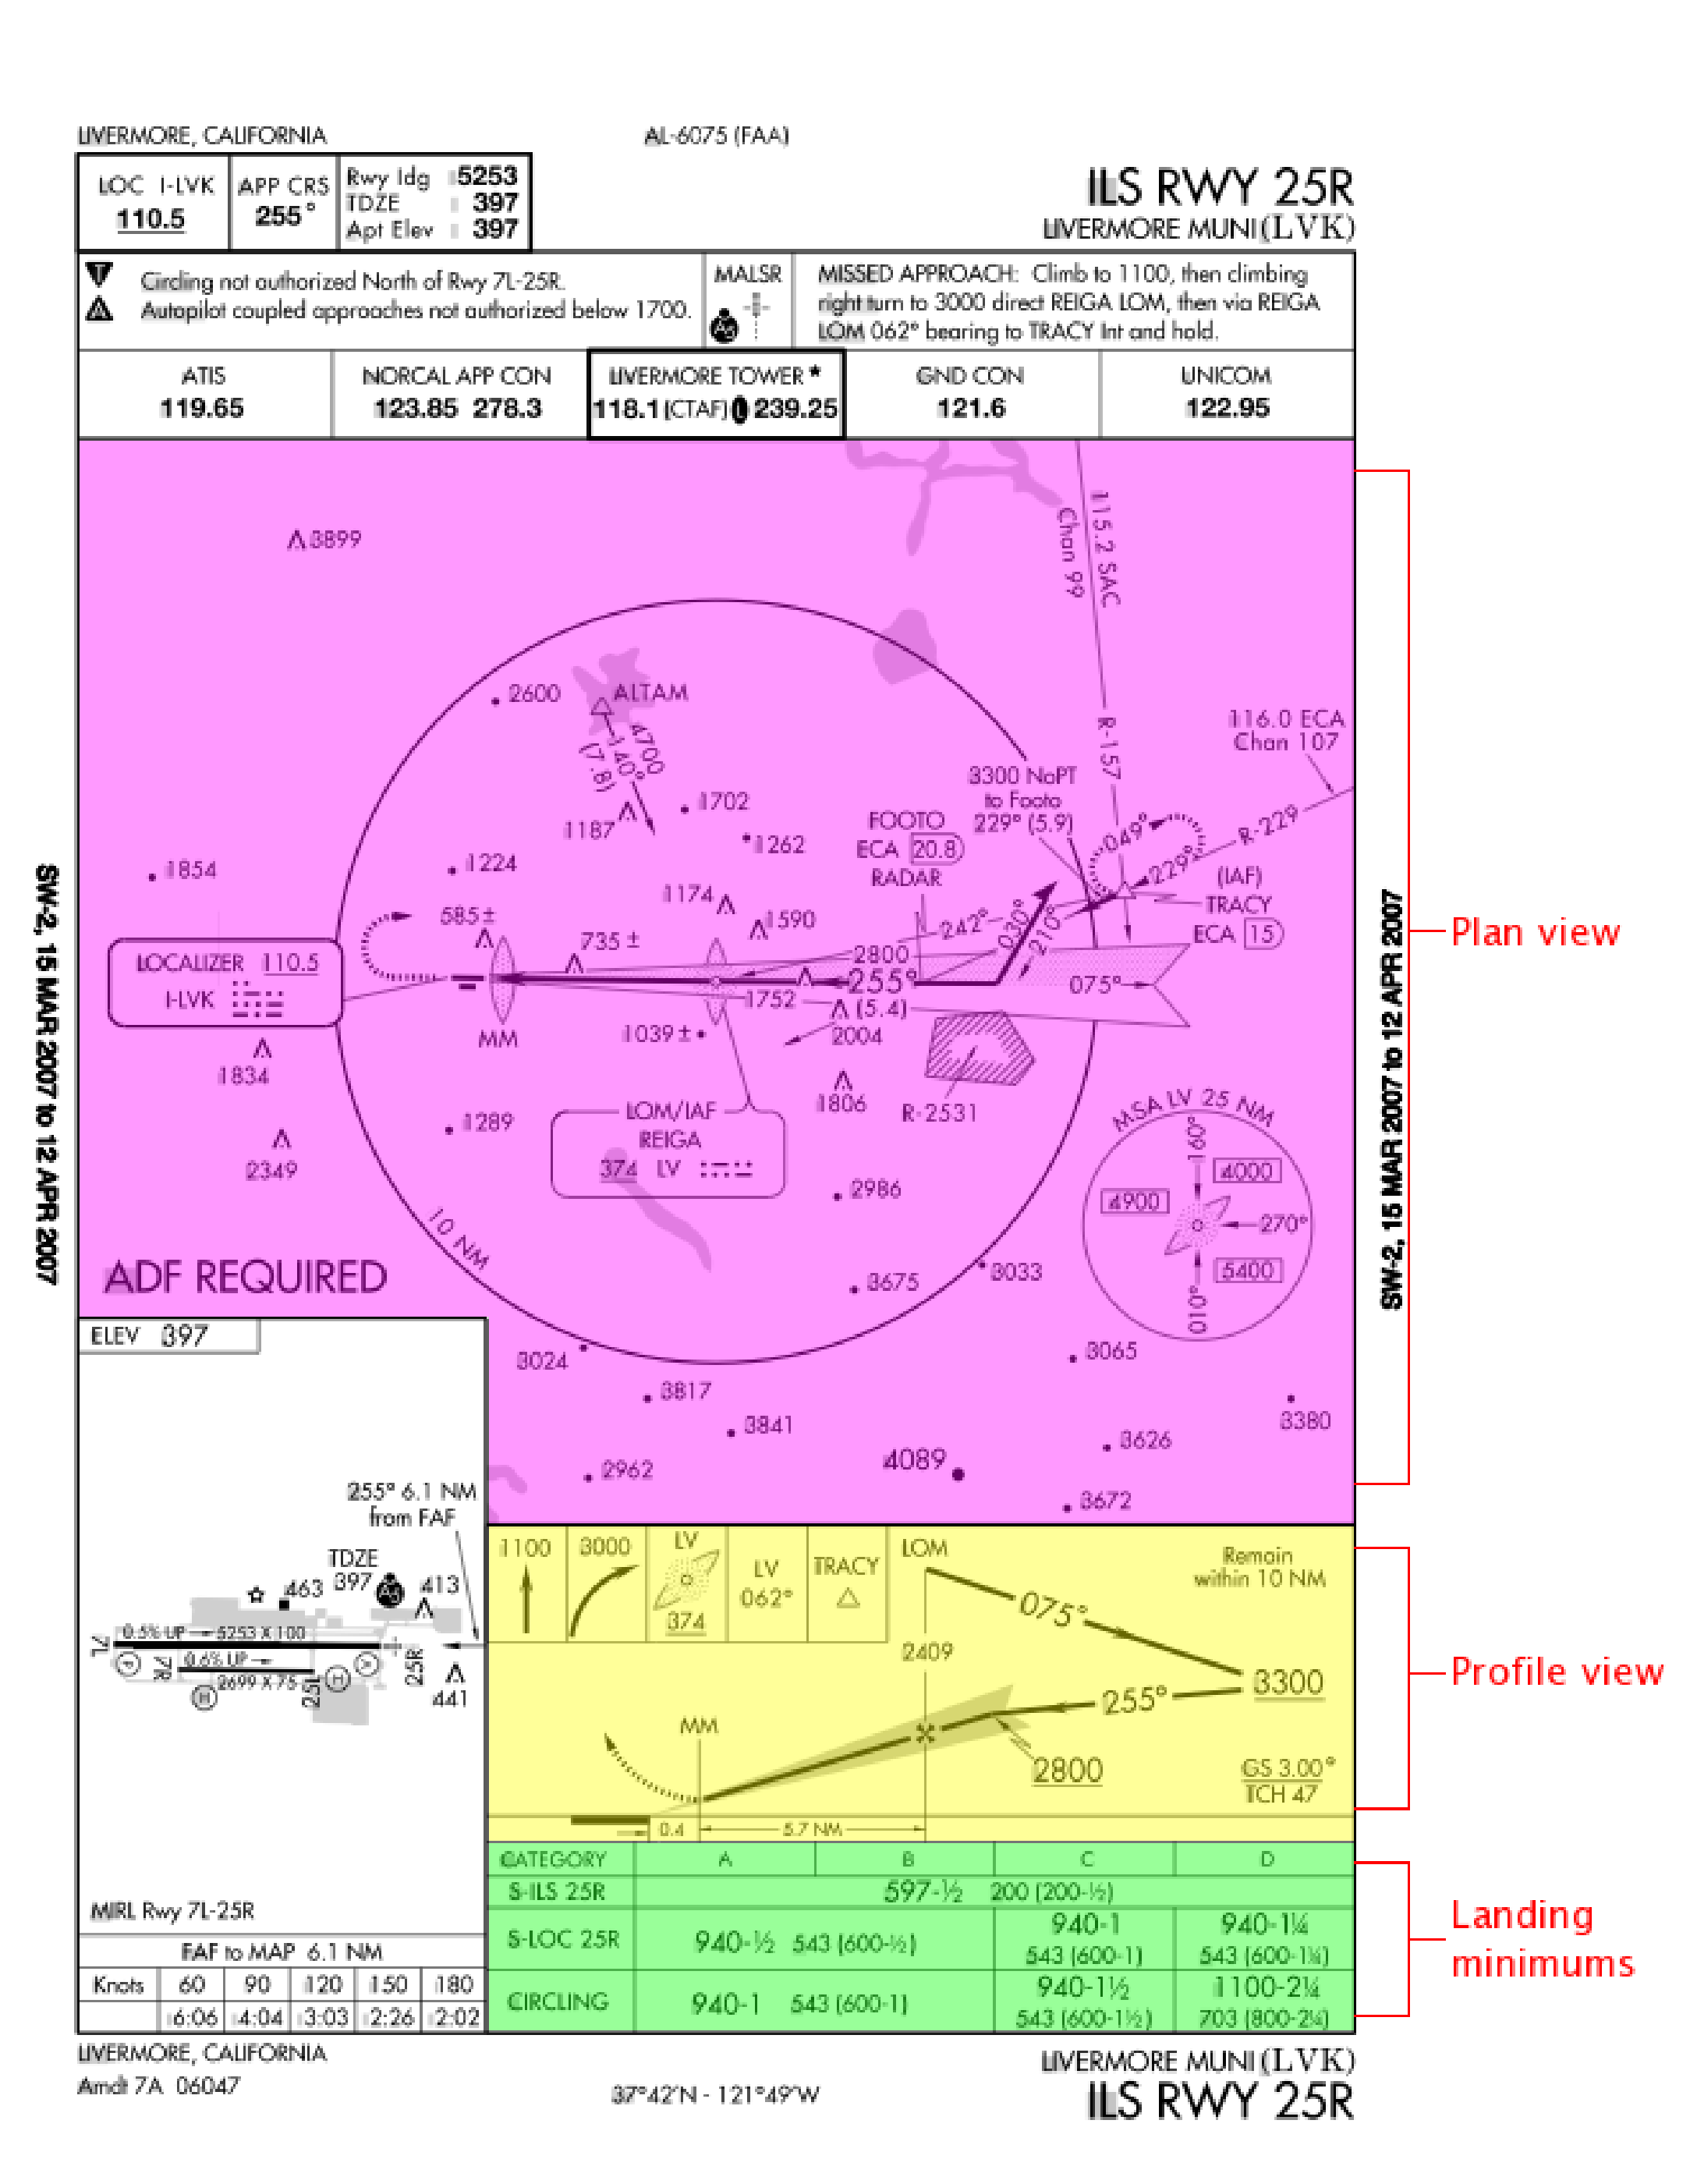
\includegraphics[width=14cm]{img/big_plate}
    \caption{利弗摩尔 25R 跑道 ILS 进近示意图}
    \label{fig:big_plate}
  \end{center}
\end{figure}

从哪里开始?首先,一个 IAP 会有一个或多个起始进近定位点(Initial Approach Fixes,IAF)。这是你进入进近程序的入口点,可以在航图的“Plan View”(平面图)里找到,也就是在图 \ref{fig:big_plate} 中用紫色标出的部分。我们的 IAP 有两个,一个是在中间,另一个是右侧(如图 \ref{fig:IAFs} 的放大)。

\begin{figure}
  \begin{center}
    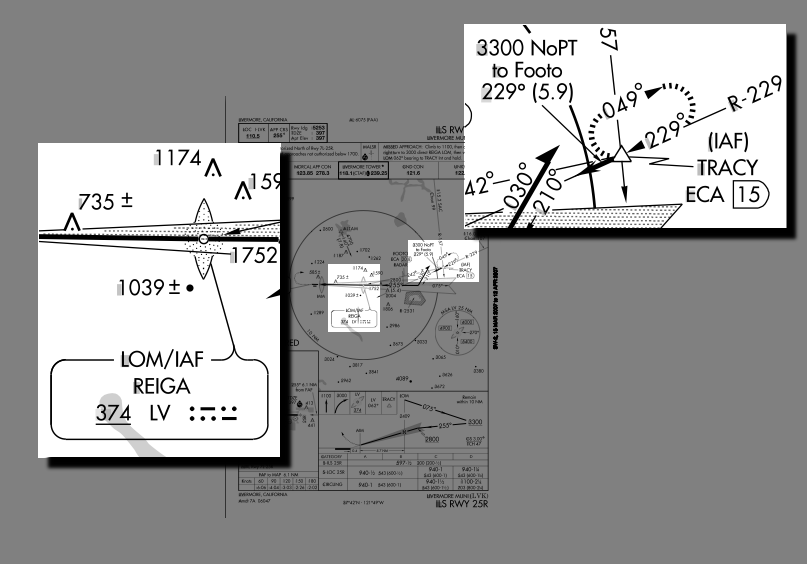
\includegraphics[width=10cm]{img/IAFs}
    \caption{起始进近点 IAF}
    \label{fig:IAFs}
  \end{center}
\end{figure}

一个 IAF 就是一个\emph{定位点(fix)},定位点是空间中的一个虚拟的点。实际上我们已经接触了另一种类型的定位点,比如 VOR 的交汇点。定位点通常也有名字(比如 MISON,SUNOL)。右侧的 IAF 称为 TRACY,由一条径向线,一个距离标识和一个高度标识合并组成。具体来说,它位于沿着 ECA(也就是 Manteca)VOR 信标台 229 度径向线,DME 15 海里(用 DME 接收机测量的 15 海里)的位置。

\subsection{无方向性信标台}

当然,我们并不使用 TRACY 作为此次飞行的 IAF,我们会使用中间的 IAF,也就是一个指点(图中的 LOM 表示“Locator Outer Marker”,外指点标),稍后再关注外指点标,目前我们集中在此定位点上。而此外指点标,则是一个 NDB(Non-directional Beacon)信标台\footnote{详情参考 \url{http://en.wikipedia.org/wiki/Non-directional_beacon}。}。它与 VOR 相似,用它可以辅助航向,并从一个地方导航到另一个地方。和 VOR 一样,它也有名字(比如此例中的 REIGA),一个频率(375 kHz),一个识别码(LV,或莫尔斯码 {\mdot\mdash\mdot\mdot\mspace \mdot\mdot\mdot\mdash})。NDB 也会在区域航图上标出,一个模糊的红色圆形,中间有很多小点点,旁边红色方框里是它的相关信息(如图 \ref{fig:NDB}。不要与旁边红色实心圆混淆,或者那个中间有字母“R”的圆形)。

\begin{figure}
  \begin{center}
    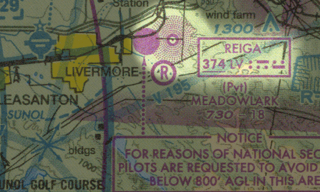
\includegraphics[width=8cm]{img/NDB}
    \caption{REIGA 无方向性信标台}
    \label{fig:NDB}
  \end{center}
\end{figure}

NDB 信标台会广播一个信号像在说“我在这里”,而飞机里的接收机会接收到这个信号并告诉飞行员,“信标台就在那里”。你只需要调节接收机频率并监视住正确的仪表。接收机,也就是 ADF(Automatic Direction Finder,自动定向设备)接收机,而相应的仪表也是 ADF,如图 \ref{fig:panel} 所示。

要调节到 REIGA,转动备用频率(STDBY)旋钮到 374。\marginpar{\textsf{ADF $\Rightarrow$ 374}} 和之前一样,鼠标中键做大幅修改(这里每次修改 100 kHz),用鼠标左键做小幅修改(1 kHz)。然后交换活动频率和备用频率(按“FRQ“按钮)。这样 374 就是选定的(SEL)频率。ADF 指针也会摆动,可能会指向右侧,也可能直指 REIGA。也许不会,为什么?因为接收机可能会处于天线模式(左上角会显示“ANT”)\footnote{天线模式,主要用来识别 NDB 信标台,因为它有较好的音频接收效果。在天线模式,ADF 指针\emph{不会}指向信标台,而是永远指向右侧。}。如果在天线模式,按 ADF 按钮,会看到显示为“ADF”。这样指针会摆向 REIGA 信标台。与 VOR 一样,为了确保我们收听到了正确的频率,需要识别信标台,因此我们将 ADF 的音频开关打开。

注意,ADF 没有 OBS,因为 ADF 的指针是指向信标台的,这太好了。这就推导出了第一个 ADF 原则:

\begin{quote}
  \begin{description}
  \item[ADF 原则 1:] 指针指向信标台
  \end{description}
\end{quote}

非常简单,事实上你也许认为者不能算是一个“原则”,但是这却是 ADF 和 VOR 的巨大差别。一台 VOR,还记得吧,追踪单一的无线电径向线,也就是你通过旋转 OBS 旋钮选择的。而一台 ADF 也有一个旋钮,也有一个一模一样的罗盘卡,也许会认为表示相同的含义。并不是,旋转这个 ADF 航向旋钮(有“HD”标签的)看看会发生什么吧。罗盘卡在移动,而指针没动。因为它\emph{只是指向信标台}。

我们现在的状况下,无论从何处飞向 REIGA,只要我们用 ADF,指针指向“就在那里”,我们就飞到“那里”,并且会飞过 REIGA 上空。然而,因为缺乏实践,又因很快就要用,我们来解释罗盘卡的用途:

\begin{quote}
  \begin{description}
  \item[ADF 原则 2 :] \emph{如果}罗盘卡指向当前航向,那么指针就表示我们\emph{飞向}信标台的航向。
  \end{description}
\end{quote}

也就是说,罗盘卡给出飞到“那里”的具体数值。

好了,这样我们就准备航向 REIGA 了。旋转 ADF 航向旋钮直到其顶部航向与当前航向一致(一般的,ADF 航向需要与方位陀螺仪航向一致)。当我们经过 SUNOL 交汇点,注意看 ADF 指针,设置方位陀螺仪的游标到那个航向(我假设你在使用自动驾驶仪,如果没有,那么只要航向那里即可)。转弯结束以后,ADF 的指针应该指向正前方\marginpar{\textsf{经过 SUNOL; 转向 REIGA}}。如果没有,那么就调整航向。\footnote{在侧风时这样做并不好,但此处忽略风的影响。}

顺便说,距离 REIGA 越近,指针就会变得越敏感,不要疯狂的让指针保持中间。只要稳定在一个航向就行,然后准备……

\subsection{程序转弯}

好了,我们飞过 REIGA,是不是直接向左转并对准跑道了?哈,如果真是这么简单就好了。我们需要向右转,\emph{飞离}机场,并做一个\emph{程序转弯}。如图 \ref{fig:PT} 中的平面图,标示出了一个虚线的程序转弯。如果你按箭头所示,需要飞离机场航向 075$^\circ$,然后左转 45$^\circ$ 到 030 $^\circ$。我们做了一个 U 字形的右转弯,远离机场。随后我们再转回 210$^\circ$,之后再右转 45$^\circ$ 到 255$^\circ$,对准跑道。这么做可以让我们有时间修正航向道,到达正确的高度,为降落 25R 做准备。

\begin{figure}
  \begin{center}
    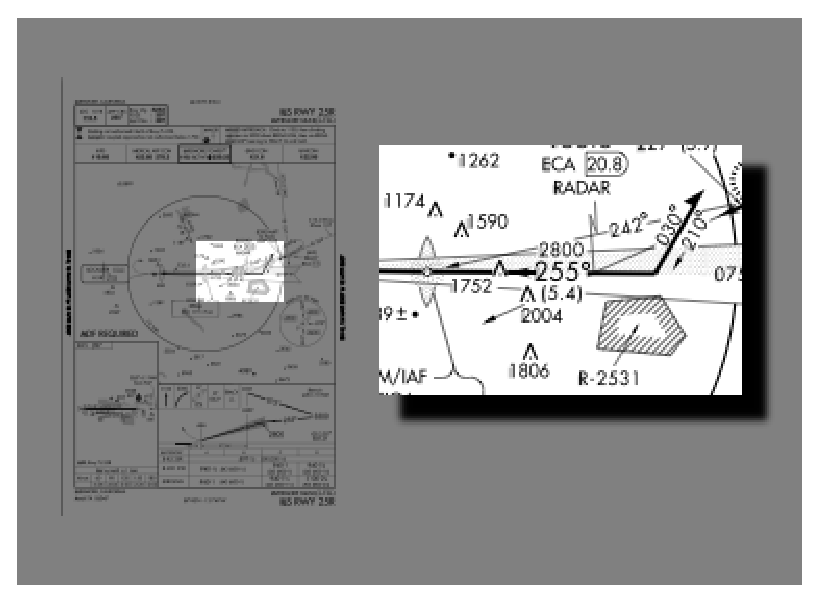
\includegraphics[width=7cm]{img/PT}
    \caption{利弗摩尔 ILS 程序转弯}
    \label{fig:PT}
  \end{center}
\end{figure}

我所说的“正确的高度”,我们如何知道呢?在图 \ref{fig:big_plate} 中黄色标注的剖面图(Profile View)部分,你可以注意到上面是 LOM,也就是我们的 IAF。跟着箭头,IAF 之后我们会航向 075$^\circ$。在程序转弯中我们下降到 3300 英尺,然而\emph{不能低于}这个高度(这就是 3300 数字\emph{下划线}的含义)。程序转弯之后航向 255$^\circ$,我们可以下降到 2800 英尺,但\emph{不能低于}这个高度,直到我们截获下滑道。

仪表进近程序并\emph{没有}告诉你程序转弯的长度。唯一要求是不能飞离 NDB 超过 10 海里。你会注意到平面图里有一个 10 海里的大圆圈。这表示“保持 10 海里以内”。这不是开玩笑。因此假设我们速度 110 节,那么每一边飞两分钟就差不多了——也就是在075$^\circ$ 飞两分钟,然后转向 030$^\circ$ 以后再飞两分钟。再往后,我们就不需要关心时间了,我们只需截获 255$^\circ$。\footnote{关于利弗摩尔机场,REIGA NDB 10 海里限制,在 2011 年 6 月新修订版航图里已经取消。——译者注}

所以,飞过 REIGA 之后,向右转 $^\circ$。我们的 ADF 有内置定时器,这样我们可以用这个来计时两分钟。按“FLT/ET”(flight time/elapsed time)按钮。中间的“FRQ”会消失,“FLT”会显示在右边,备用频率会被定时器替代。现在表示全部飞行时间,不能修改,除非重新换电池。再次按“FLT/ET”按钮,你会看到“ET”显示出来了,还有一个时间,可能会与飞行时间相同,要重置此预计时间,按旁边的“SET/RST”按钮。这样定时器会归零,然后来时计时(见图 \ref{fig:ADF})\footnote{定时器也可以设置成倒数计时模式,这里并没有实现。}。在计时模式,当你按“SET/RST”按钮,计时器都会归零。若此时想看备用频率,按一次“FRQ”按钮,计时器持续计时。

\begin{figure}
  \begin{center}
    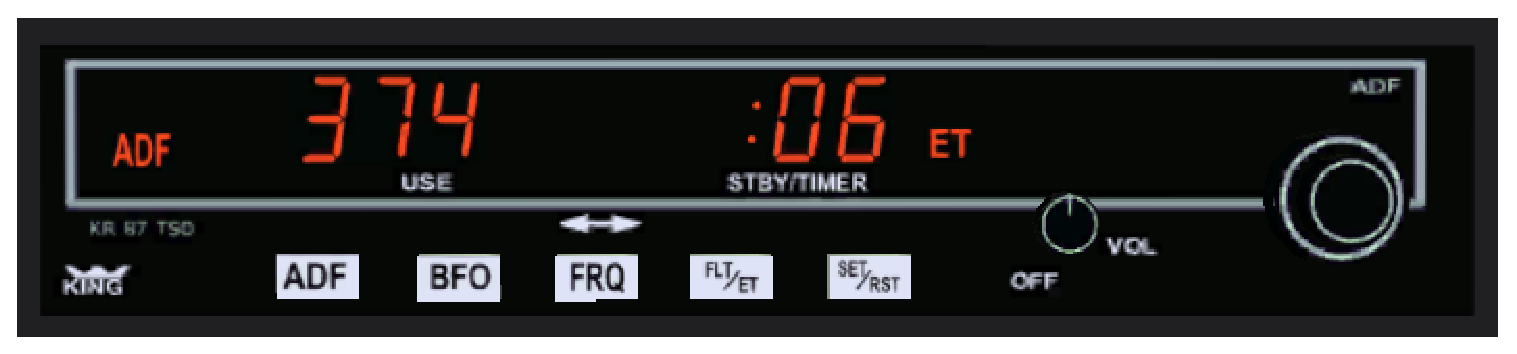
\includegraphics[width=7cm]{img/ADF}
    \caption{定时器运行时的 ADF}
    \label{fig:ADF}
  \end{center}
\end{figure}

\subsection{追着指针}



%%%%%%%%%%%%%%%%%%%%%%%%%%%%%%%%%%%%%%%%%%%%%%%%%%%%%%%%%%%%%%%%%%%%
\fi
%%%%%%%%%%%%%%%%%%%%%%%%%% ENGLISH VERSION %%%%%%%%%%%%%%%%%%%%%%%%%
\iffalse
\chapter{An IFR Cross Country Flight Tutorial}
\label{IFR Tutorial}

\section{Introduction}

\begin{figure}[h]
  \begin{center}
    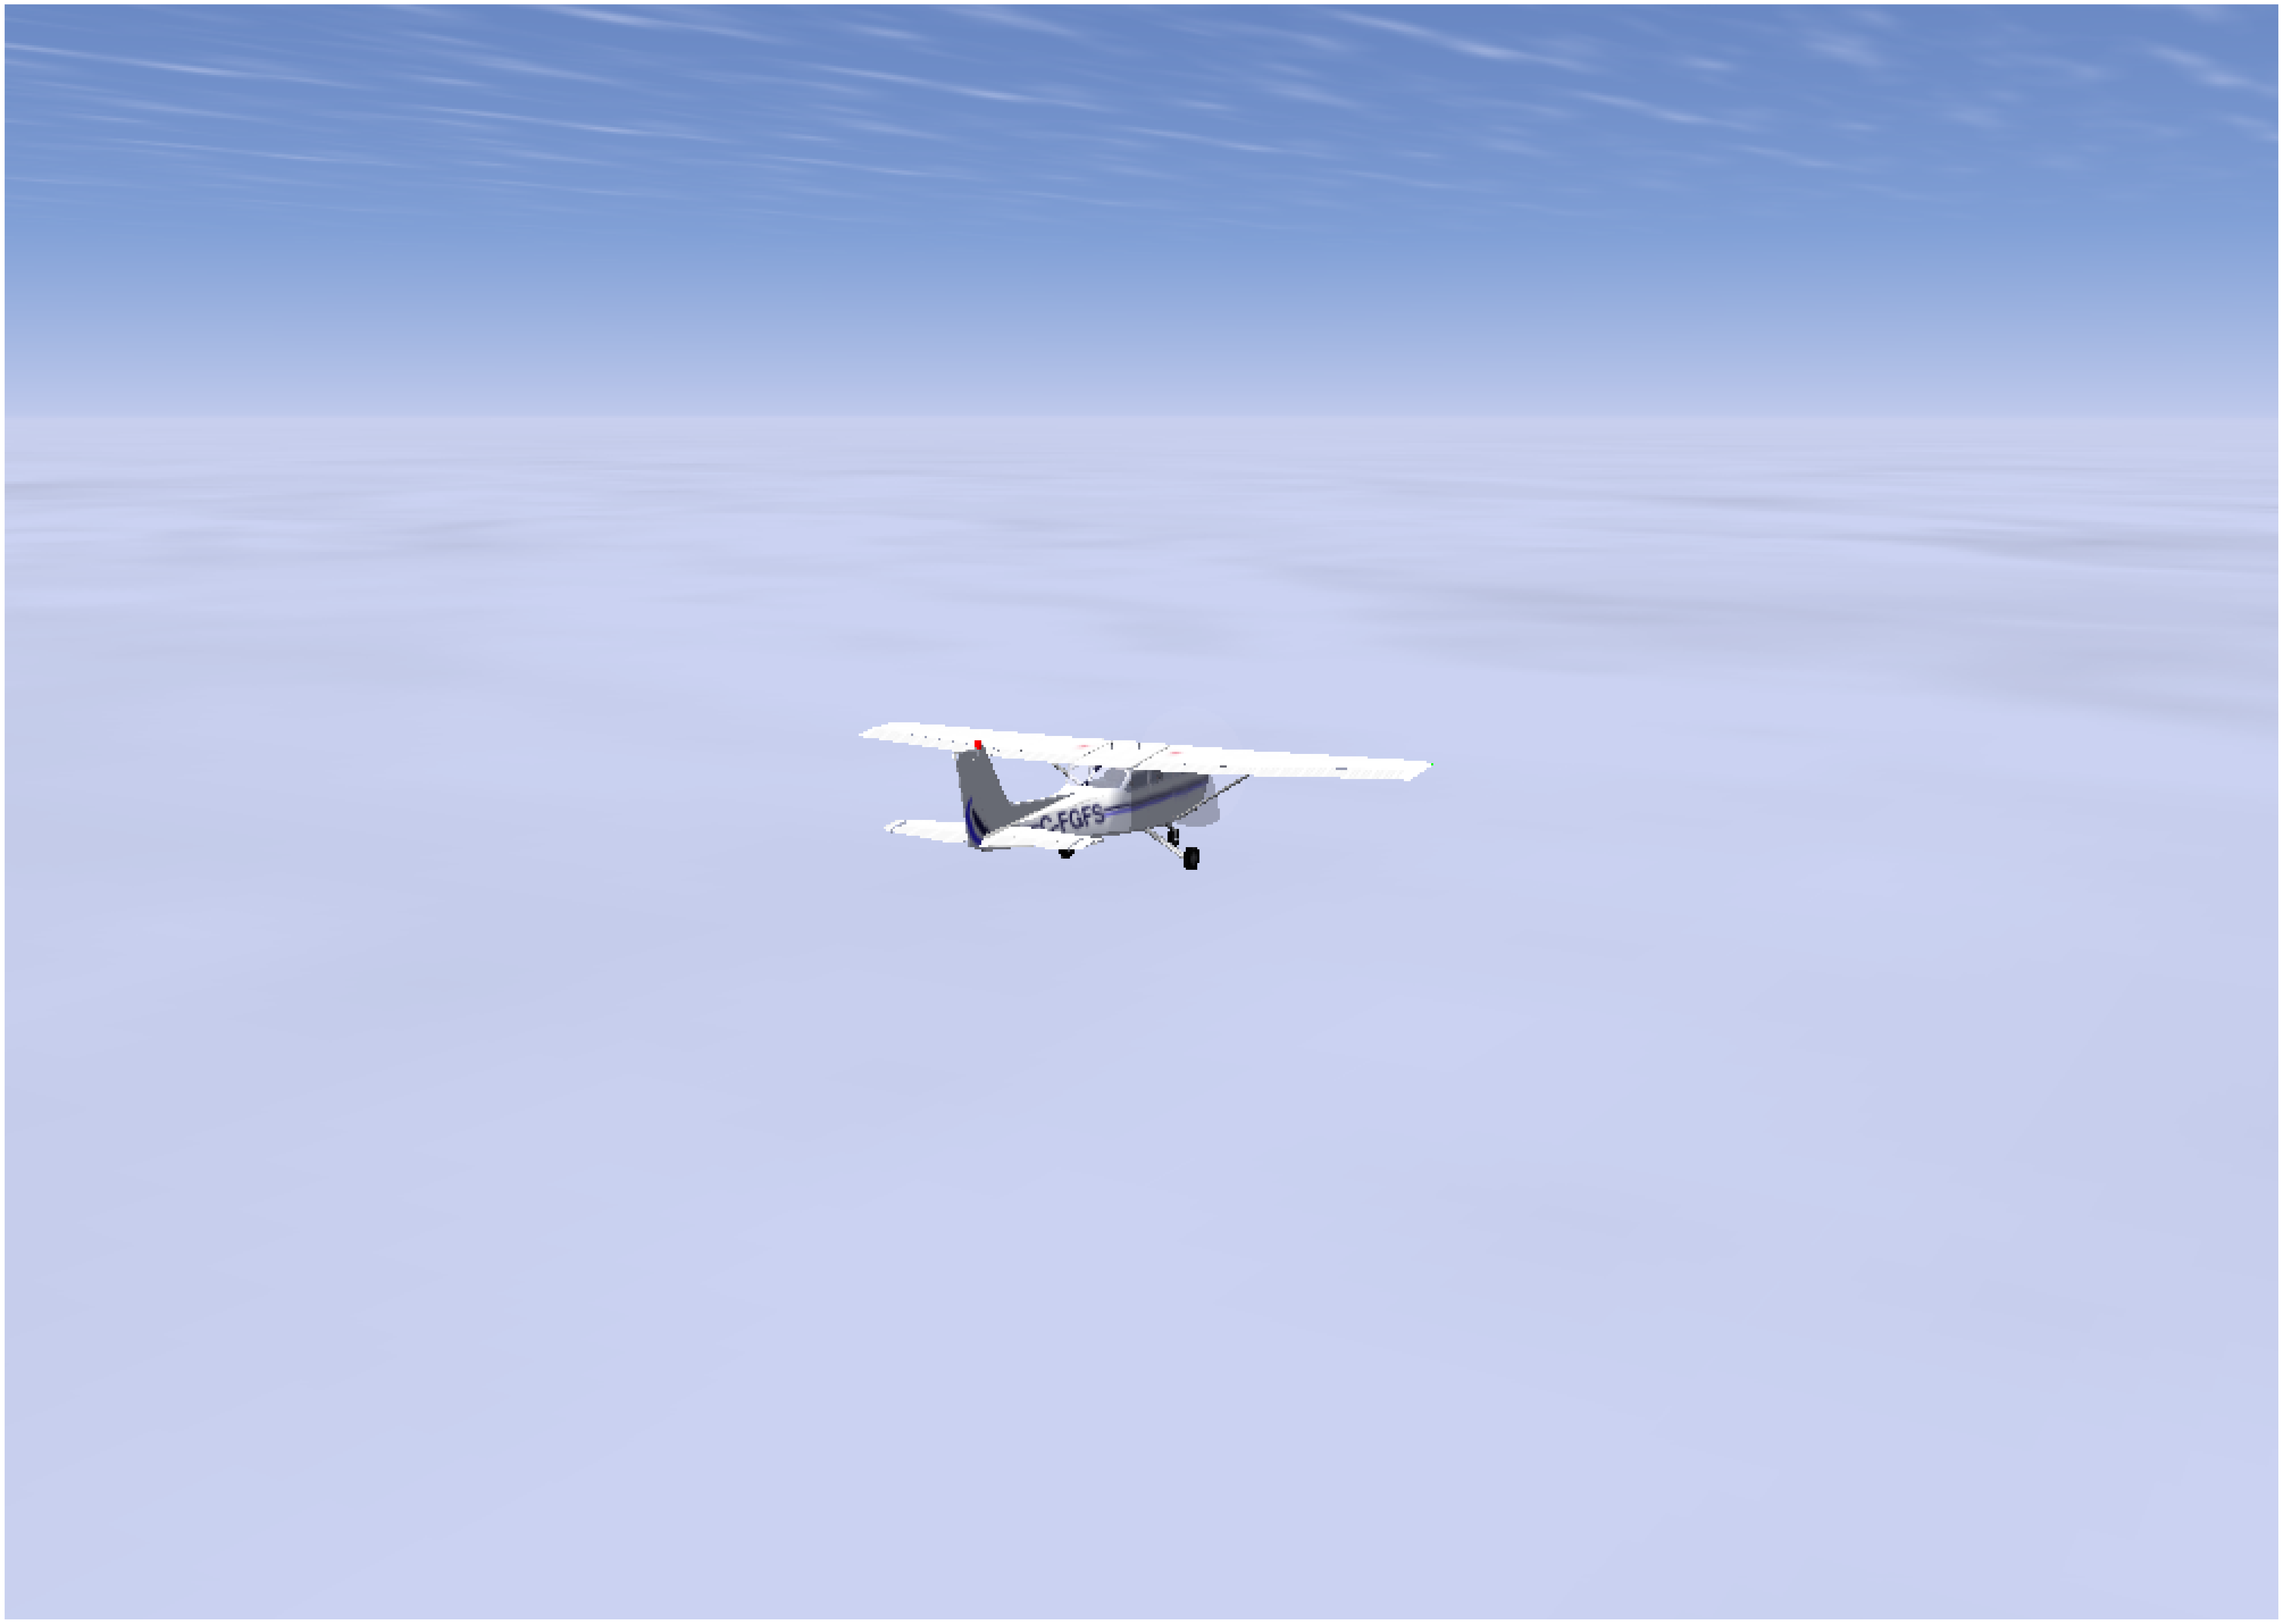
\includegraphics[width=6cm]{img/somewhere}
    \caption{Flying over the San Antonio Dam to Livermore.  I think.}
    \label{fig:somewhere}
  \end{center}
\end{figure}

In the cross country flight tutorial, you learned about VFR flight,
and in the course of the flight you were introduced to most of the
flight instruments in the C172p.  Now we're going to do an Instrument
Flight Rules (IFR) flight.  In this flight you'll be introduced to the
remaining instruments, learn a bit about IFR flight, and learn many,
many TLAs (Three-Letter Acronyms).

We'll fly the same flight, from Reid-Hillview (KRHV), runway 31R, to
Livermore (KLVK), runway 25R, only this time we'll do it in IFR
conditions: a ceiling 200 feet above ground level, and 800 metre
visibility.  This tutorial assumes you've completed the cross country
flight tutorial.
\subsection{Disclaimers}

This is not intended to teach you how to fly IFR.  Rather, it is meant
to give a flavour of what IFR flying is like, and remove the mystery
of the panel instruments not covered by the cross country flight
tutorial.

I'm not a pilot.  Like the previous tutorial, this information has
been gleaned from various non-authoritative sources.  If you find an
error or misunderstanding, please let me know.  Mail me at
bschack-flightgear -at- usa -dot- net.

This flight was flown using FlightGear 3.0.  Newer or older versions
of FlightGear might be slightly different.

\section{Before Takeoff}

We need to tell FlightGear about our flight conditions.  There are
different ways to set our ``desired'' weather, but we'll use the
global weather menu.  After launching FlightGear, click
\textbf{\textsf{Environment}} $\Rightarrow$ \textbf{\textsf{Weather}}
to bring up the weather dialog.  In the \textbf{\textsf{Weather
    Conditions}} list, select \textbf{\textsf{CAT I minimum}}.

This will give us a low ceiling and reduced visibility.
Unfortunately, it will also give us rather stiff winds.  If you don't
want to deal with them, then you can easily turn off the winds:

\begin{itemize}
\item Click on \textbf{\textsf{Weather Conditions}} again, and select
  \textbf{\textsf{Manual input}}.
\item In the METAR string at the bottom, change ``15015KT'' (15 knot
  winds coming from 150$^\circ$) to ``15000KT'' (0 knot winds coming
  from 150$^\circ$).
\end{itemize}

Hit \textbf{\textsf{OK}} to make FlightGear accept the changes and
close the dialog.  

Finally, I find that the reduced visibility situations are rendered
best when atmospheric light scattering is turned off: click
\textbf{\textsf{View}} $\Rightarrow$ \textbf{\textsf{Rendering
    Options}} and make sure the \textbf{\textsf{Atmospheric light
    scattering}} box is unchecked.

% Porco Rosso!

% Note: If I change the visibility while cruising, the autopilot
% momentarily spazzes.  What's with that?

% What are VFR minimums?  3 miles visibility, and basically 1000'
% ceiling (actually, 500 feet below the clouds, and since the minimum
% flight altitude is 500 feet AGL, that means at least 1000.
% Furthermore, you need to clear obstacles near cities by 1000 feet,
% so near cities, you need 1500' AGL).

% EYE - we need to create real references to the Cross Country Flight
% Tutorial.

\begin{figure}
  \begin{center}
    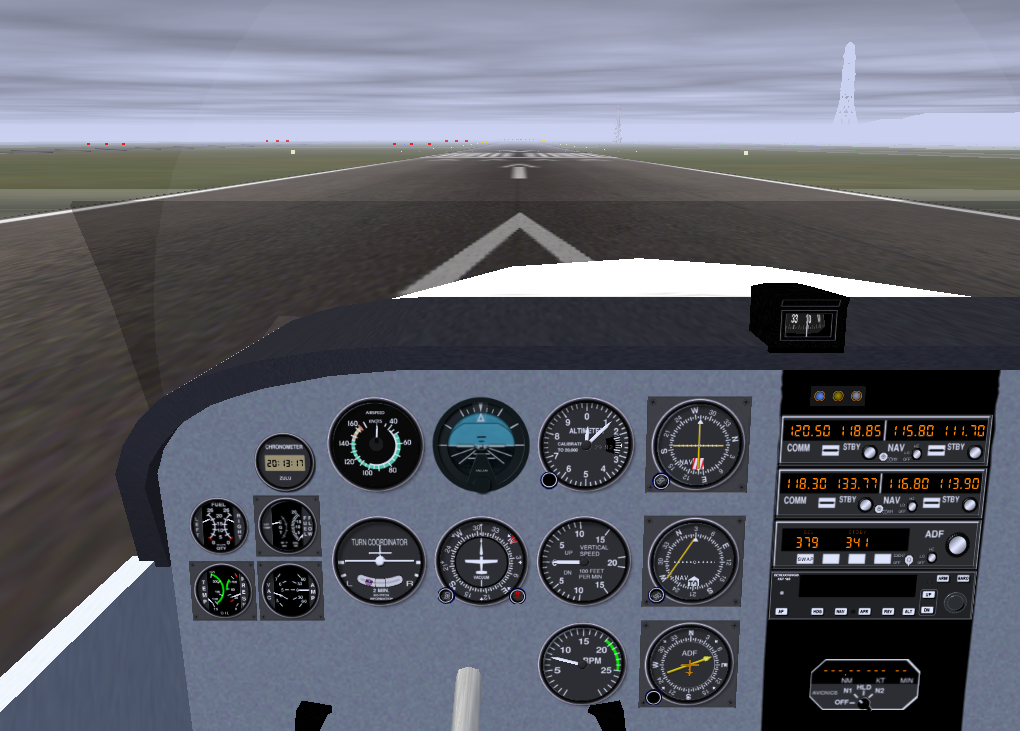
\includegraphics[width=10cm]{img/KRHV}
    \caption{On runway 31R at KRHV}
    \label{fig:KRHV}
  \end{center}
\end{figure}

\subsection{Flight Planning}

When you look out the window, you'll see something like Figure
\ref{fig:KRHV}.  Those clouds don't look very friendly, and it's hard
to even see past the end of the runway.  Maybe we should just
\emph{drive} there in the Cessna.  We had been planning to practice
ground steering anyway \ldots{}

So how do you get from A to B when you can't see?  There are a variety
of ways that have evolved over the years, with various advantages and
disadvantages.  Our flight will use all of the navigation instruments
the standard Cessna C172p has, just to give a taste of what's
possible.

Our entire route, and the aids we'll be using, are shown in
Figure \ref{fig:sectional_labelled}.  Our route is in green, the
navigational aids blue and red.  The route looks a bit crazy --- in
fact, you might wonder if we're \emph{more} lost using our fancy
equipment than just flying by the seat of our pants --- but there is a
method to the madness.  Rather than overwhelming you with details by
explaining it all now, I'll explain it bit by bit as we go along.

\begin{figure}
  \begin{center}
    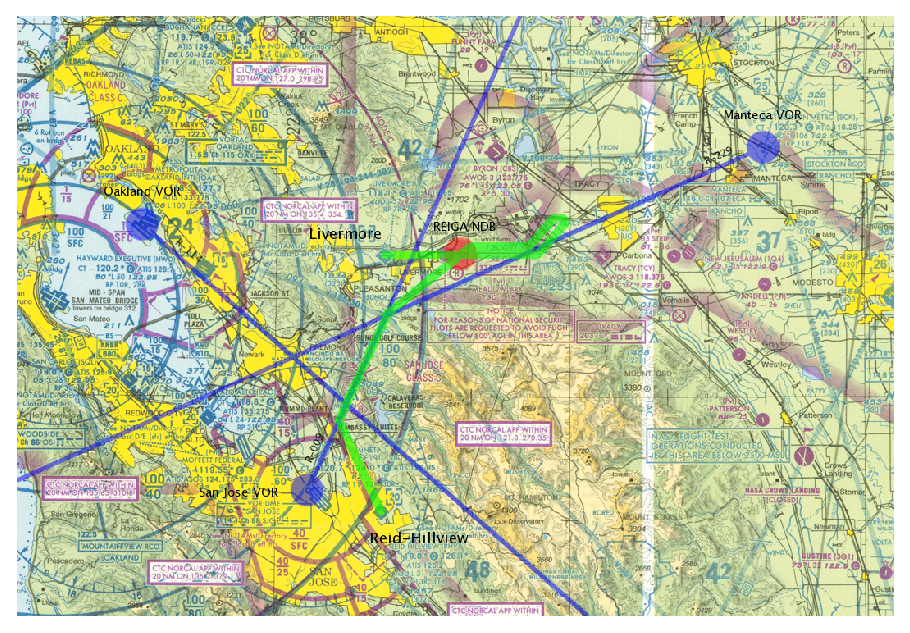
\includegraphics[width=20cm, angle=-90]{img/sectional_labelled}
    \caption{Green: our route, Blue: VORs and radials, Red: NDBs}
    \label{fig:sectional_labelled}
  \end{center}
\end{figure}

% IFR sectionals?

\subsection{VHF Omnidirectional Range}

The first bit will involve VOR\footnote{See
  \url{http://en.wikipedia.org/wiki/VHF_omnidirectional_range} for
  more information.} (VHF (Very High Frequency) Omnidirectional Range)
navigation, and will get us to a point about 5 nm (nautical miles)
south of Livermore.

VOR stations are indicated on the sectional by a big bluish-green
circle with compass markings around the outside.  I've helped you by
marking their centers with a big blue dot as well.  Reid-Hillview is
very close to one, San Jose, which you can see in Figure
\ref{fig:sectional_labelled}.  Near the centre of the circle, in a
bluish-green rectangle, is the station information.  According to the
station information, it's a VOR-DME station (I'll explain DME later),
its name is San Jose, its frequency is 114.1 MHz (or Channel 88, which
is an alternative way to say the same thing), and its identifier, or
``ident'', is SJC (which in Morse code is \mdot\mdot\mdot\mspace
\mdot\mdash\mdash\mdash\mspace \mdash\mdot\mdash\mdot).

% In emacs, try M-x morse-region on SJC
% .../.---/-.-.

To tune into a VOR station, we use one of the NAV receivers, which are
paired with the COMM receivers (see Figure \ref{fig:panel}).  And we
navigate using the corresponding VOR gauge.  We'll choose the NAV1
receiver (and VOR1 gauge) in this case (NAV2 would have worked just as
well).  Before setting the frequency, check out the VOR1 gauge.  It
should look like VOR1 on the left in Figure \ref{fig:VOR1}.  The
important thing is the red ``NAV'' flag.  That means there's no VOR
signal, so we can't trust the gauge.

\begin{figure}
  \begin{center}
    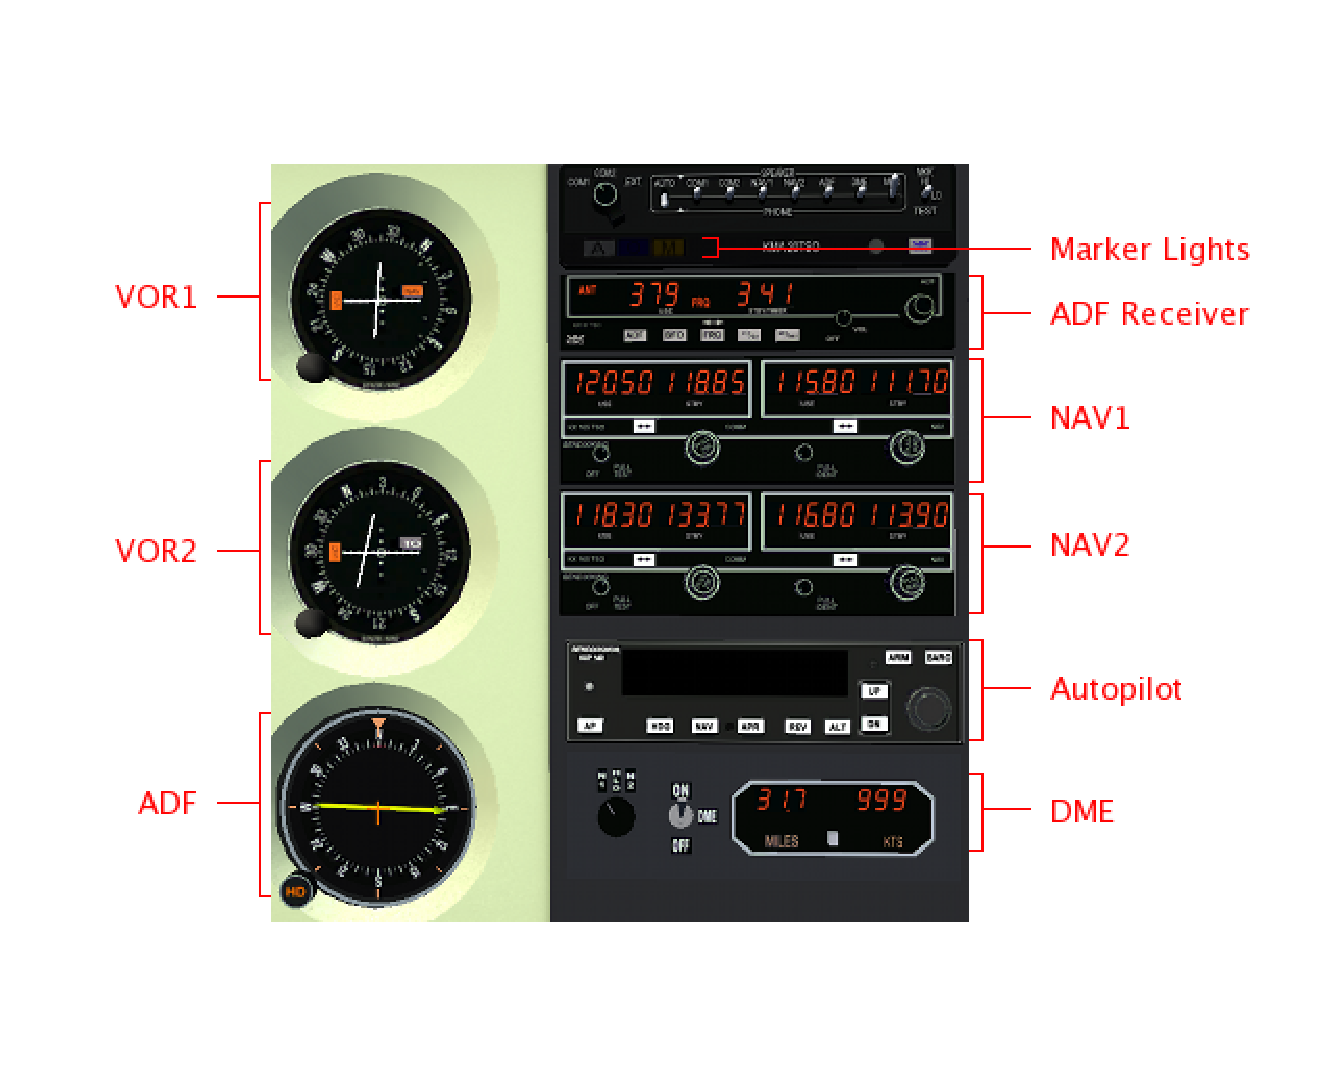
\includegraphics[width=12cm]{img/panel_labelled}
    \caption{IFR navigation instruments}
    \label{fig:panel}
  \end{center}
\end{figure}

The NAV receiver has an active frequency, a standby frequency, and a
tuning knob, just like the COMM receiver.\footnote{Operation of the
  COMM receivers was covered in the cross country flight tutorial.}
Tune it to 114.1, and press the swap button\marginpar{\textsf{NAV1
    $\Rightarrow$ 114.1}\footnotemark}\footnotetext{All important
  actions and events will be given in the margin.  This should provide
  a nice summary of the flight, uncluttered by the verbiage of the
  text.}.  If you look at VOR1, you should notice that the red ``NAV''
flag has disappeared, to be replaced with a ``TO'' flag, as shown on
the right of Figure \ref{fig:VOR1}.  That means we're receiving a
signal.  But is it the correct one?  What if we accidentally set the
wrong frequency?

\begin{figure}
  \begin{minipage}[b]{0.5\linewidth}
    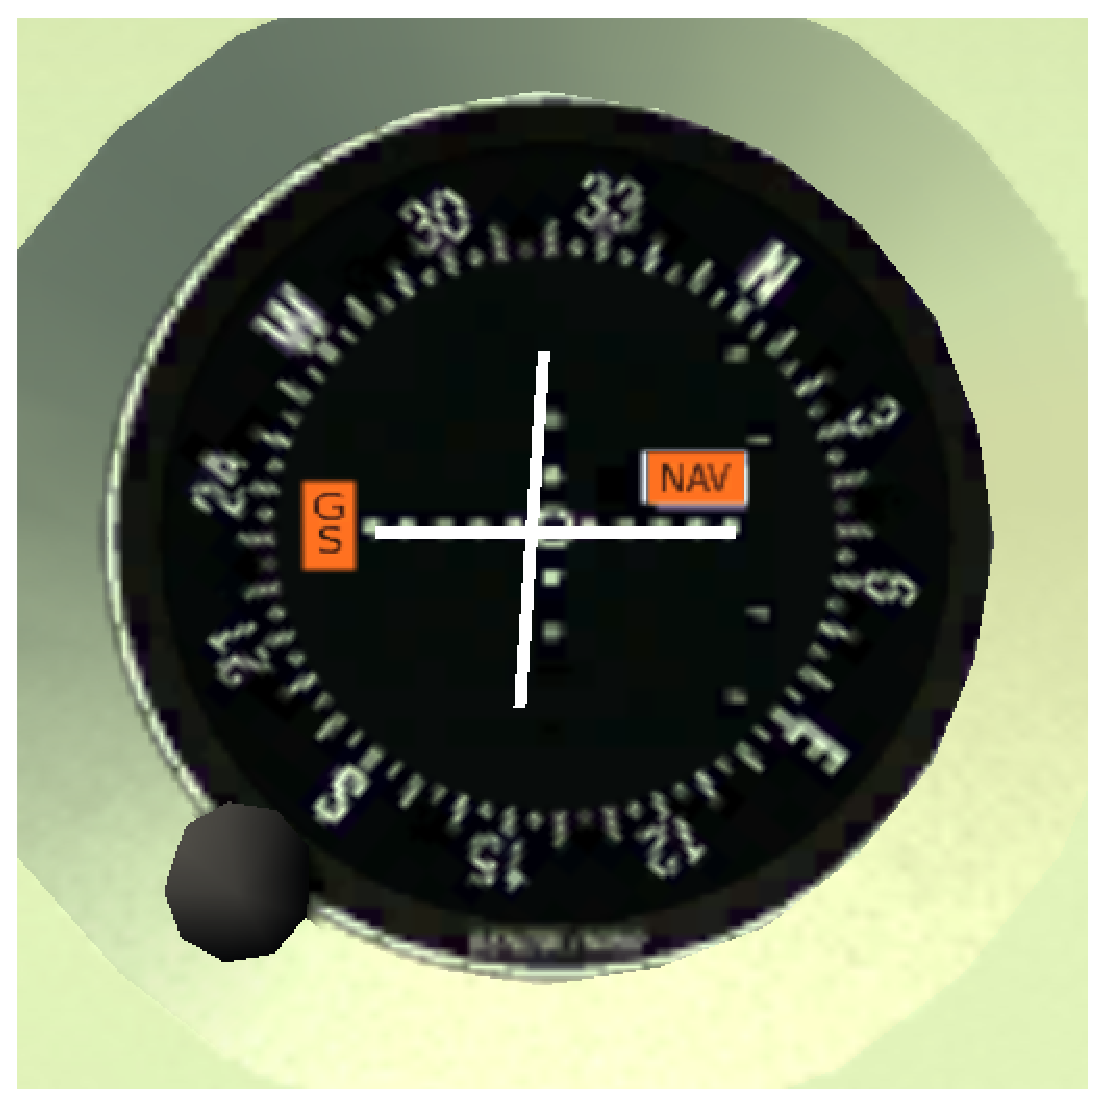
\includegraphics[width=6cm]{img/VOR1_before}
  \end{minipage}
  \hspace{0.5cm}
  \begin{minipage}[b]{0.5\linewidth}
    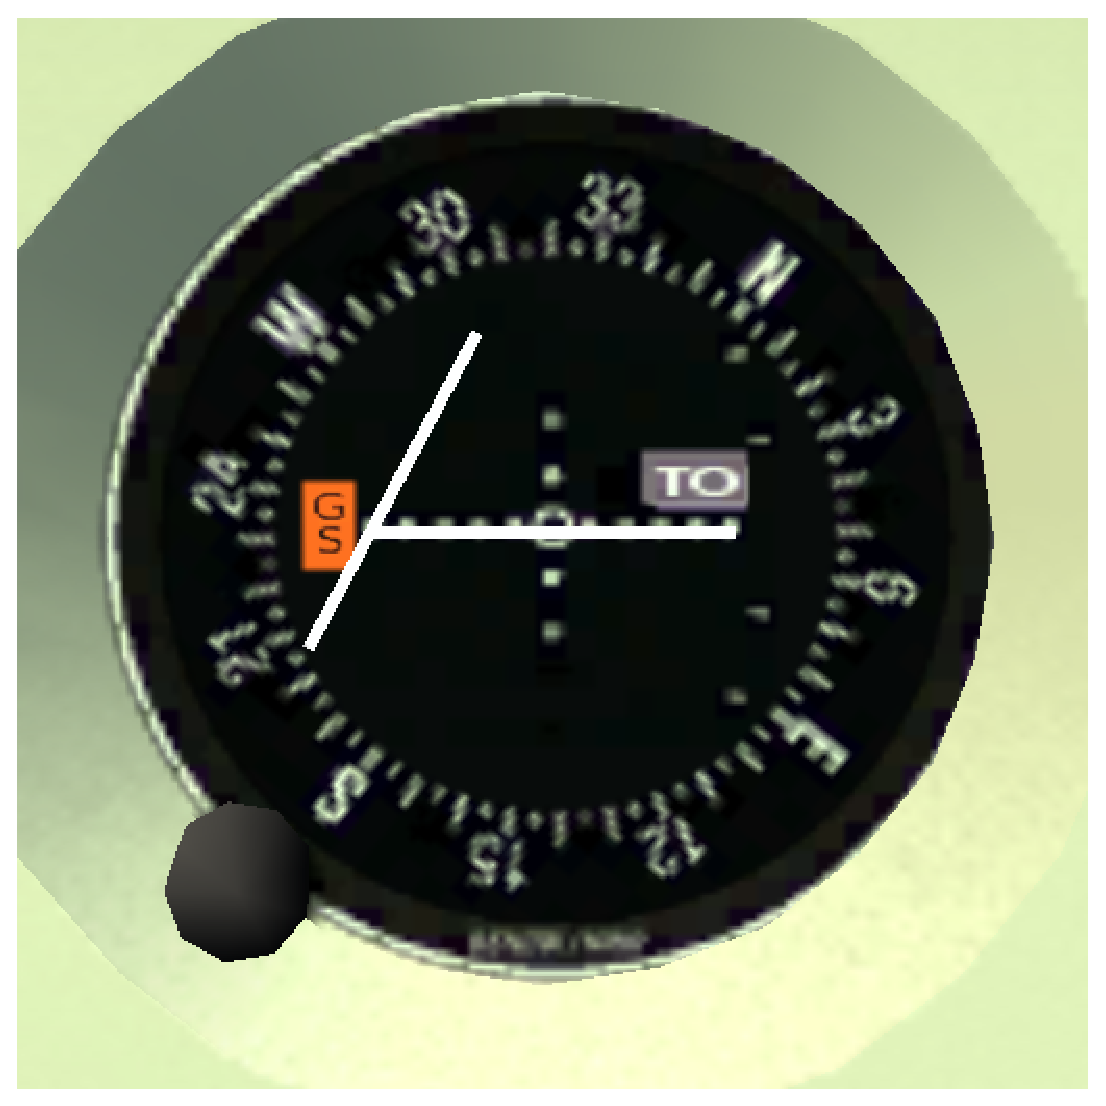
\includegraphics[width=6cm]{img/VOR1_after}
  \end{minipage}
  \caption{VOR1, before and after tuning}
  \label{fig:VOR1}
\end{figure}

To confirm that we're tuned into the correct VOR, we listen for its
ident.  If you can't hear the ident, or if it doesn't match the chart,
don't trust the needle.  So far, you probably haven't heard a thing.
Why?  Check the audio panel (see Figure \ref{fig:panel}).  You'll note
there's a switch for all the instruments that produce useful sounds,
and NAV1 is one of them.  Flip the switch up (or down --- it doesn't
matter), and you should hear this: \mdot\mdot\mdot\mspace
\mdot\mdash\mdash\mdash\mspace \mdash\mdot\mdash\mdot.\footnote{Still
  can't hear it?  Check the volume control on the NAV1 receiver.  If
  that has no effect, click \textbf{\textsf{File}} $\Rightarrow$
  \textbf{\textsf{Sound Configuration}} and adjust the settings.  If
  that doesn't work, check the volume on your computer.  If that
  doesn't work, and you have external speakers, adjust the volume on
  the speakers.  And if that doesn't work, check your ears.} Nice.
Flip the switch back to the centre when you get tired of listening to
dots and dashes.

% EYE - talk about volume knobs on receivers?

% SJC = .../.---/-.-.

% EYE - \circ is ugly in \emph{}!  I need a real degree symbol!
Back to VOR1.  There's a knob on the lower left, called the OBS (Omni
Bearing Selector).  As the name vaguely suggests, it is used to select
a bearing.  If you turn it, you should see the vertical needle, called
the CDI (Course Deviation Indicator) move.\footnote{The horizontal
  needle is used in ILS landings, which will be explained later.}  Try
to center the needle.  It should center when the little arrow at the
top points to somewhere around 277.  That number, and the TO flag
means: ``Flying at a heading of \emph{277$^\circ$} will lead you
directly \emph{to} the station''.

That's great, except, according to our route, we don't want to go
\emph{to} the station.  We actually want to intercept the light blue
line labelled ``009$^\circ$'' (the ``9 degree radial'') coming
\emph{from} the station.  How do we do that?  Simple.  Set the OBS to
9\marginpar{\textsf{VOR1 OBS $\Rightarrow$ 009}}.  When we fly across
the radial, the needle will center, and the flag will say FROM.  This
tells us: ``flying at a heading of \emph{9$^\circ$} will lead you
directly away \emph{from} the station'', which is what we want.  At
that point we'll turn right to a heading of 9$^\circ$.

% EYE - explain the bug?
One final thing --- set the heading bug on the directional gyro to our
current heading (about 310$^\circ$)\marginpar{\textsf{Heading bug
    $\Rightarrow$ 310}}.

\subsection{How High Are We Really?}

One effect of our changing the weather conditions is that the
barometric pressure is no longer the standard value of 29.92.  Our
altimeter needs to know the correct value, otherwise it will report
the wrong altitude.  This isn't critical at takeoff, but it can make a
\emph{huge} difference when descending through the clouds (can you say
``controlled flight into terrain''?).

As described in the cross-country flight tutorial, we get the current
barometric pressure via ATIS.  To recap, click \textbf{\textsf{AI}}
$\Rightarrow$ \textbf{\textsf{ATC Services in Range}}, select our
airport, and look up the ATIS frequency (it should be 125.20 MHz).
Dial this frequency into COMM1 or COMM2 (remembering to flip the
appropriate switch on the audio panel), listen to the ATIS report, and
set the altimeter to the given barometric pressure.

We are going to be using the autopilot (see Figures \ref{fig:panel}
and \ref{fig:ap_vs}) to hold an altitude (more on that later), so it
also needs to know the barometric pressure.  To do so, click the BARO
button on the autopilot.  You should see ``29.92'' displayed --- this
is what the autopilot thinks the barometric pressure is.  Before the
``29.92'' disappears (within about 3 seconds), rotate the big dial to
change it to the correct value.

\section{Takeoff}

We're ready to take off.  There are other preparations that we should
have made, but again, in the interests of not overwhelming your
brains, I'm only feeding you a bare minimum of information, and
feeding it in trickles.  This brings us to the most important control
you have --- the `p' key.  Use this often, especially when a new
concept is introduced.

Okay.  Take off, keeping a heading of 310$^\circ$ for
now\marginpar{\textsf{Take off; climb on runway heading}}.  Establish
a steady rate of climb.  We plan to climb to 4000 feet.  There's just
one problem though --- those ugly-looking clouds are standing in our
way.

\section{In the Air}

If this is your first attempt at IFR flight, you will find it
impossible to fly once you enter the clouds.  When you enter the
clouds, you will be momentarily disconcerted by the lack of visual
cues.  ``No matter,'' you then think.  ``I'll just keep things
steady.''  In a few moments, though, you'll probably notice dials and
needles spinning crazily, and without knowing it, you'll be flying
upside down, or diving towards the ground, or stalling, or all three.

It takes practice to get used to flying without external visual clues,
although it's a skill that you definitely \emph{must} master if you
want to fly IFR.  For now though, we'll use ``George'', the autopilot,
to make this part of flying easier.

\subsection{George I}

Once you've established a steady rate of climb and heading, engage the
autopilot by pressing the AP button.  You should see ``ROL'' displayed
on the left to show that it's in ``roll mode'' --- it is keeping the
wings level.  In the middle it will display ``VS'', to show it is in
``vertical speed'' mode --- it is maintaining a constant vertical
speed.  On the right it will \emph{momentarily} display that vertical
speed (in feet per minute).  Initially, the value is your vertical
speed at the moment the autopilot is turned on.  In the case of Figure
\ref{fig:ap_vs}, the autopilot has set the vertical speed to 300 feet
per minute.

\begin{figure}
  \begin{center}
    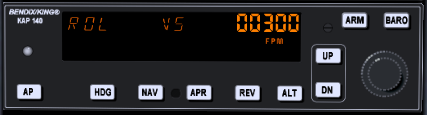
\includegraphics[width=7cm]{img/ap_vs}
    \caption{Autopilot after engaging}
    \label{fig:ap_vs}
  \end{center}
\end{figure}

% EYE - is it a bug?

When you engage the autopilot, CHECK THIS CAREFULLY.  Sometimes the
autopilot gets a very funny idea about what your current rate of climb
is, like 1800 feet per minute.  Our little Cessna cannot sustain this,
and if the autopilot tries to maintain this (and it will), you will
stall before you can say ``Icarus''.  This is a bug, to be sure, and a
bit annoying, but it is also a useful cautionary lesson --- don't put
blind faith in your equipment.  Things fail.  You have to monitor and
cross-check your equipment, and be prepared to deal with problems.

We want a vertical speed of around 500 to 700 feet per minute.  Hit
the up and down (UP and DN) buttons to adjust the vertical speed to a
nice value.  Take into account the airspeed as well.  We want a
sustainable rate of climb.

Finally, once you're climbing nicely, hit the heading (HDG)
button\marginpar{\textsf{Engage autopilot; set vertical speed; engage
    heading mode}}.  On the display, ``ROL'' will change to ``HDG'',
and the autopilot will turn the airplane to track the heading bug.
Since you set the heading bug to the runway heading, and you took off
straight ahead (didn't you?), it shouldn't turn much.

\subsection{MISON Impossible}

It's around 8 nm to the 009 radial intercept, so we've got a bit of
time.  Since there's no scenery to admire (eg, see Figure
\ref{fig:murk}), we might as well prepare for the next phase of the
flight.

\begin{figure}
  \begin{center}
    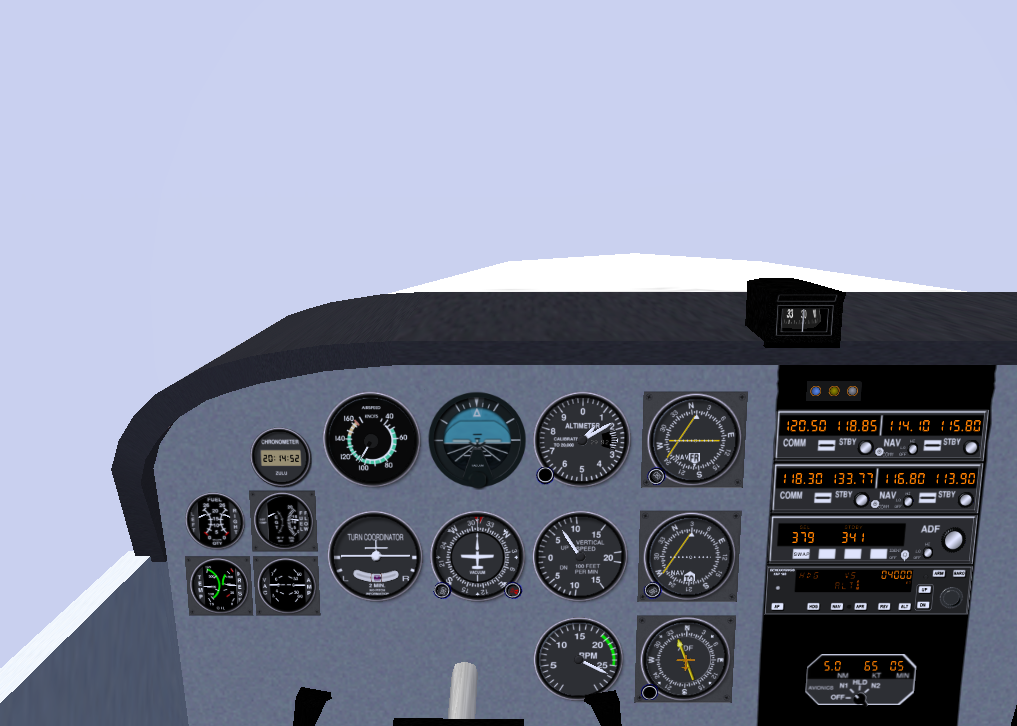
\includegraphics[width=6cm]{img/murk}
    \caption{Typical IFR scenery}
    \label{fig:murk}
  \end{center}
\end{figure}

If you look along our route, just after we intercept the 009 radial
and turn north, we pass by a point labelled MISON (see Figure
\ref{fig:Oakland} for a closeup of that section of the chart without
my fat blue and green lines drawn on top.  MISON is in the lower
right).  Just above and to the left of MISON are two crossed arrows.
MISON is an intersection.  We're actually going to pass east of MISON,
but the radial passing roughly from northwest to southeast through
MISON (and our route) is of interest to us.  We're going to use it to
monitor our progress.

\begin{figure}
  \begin{center}
    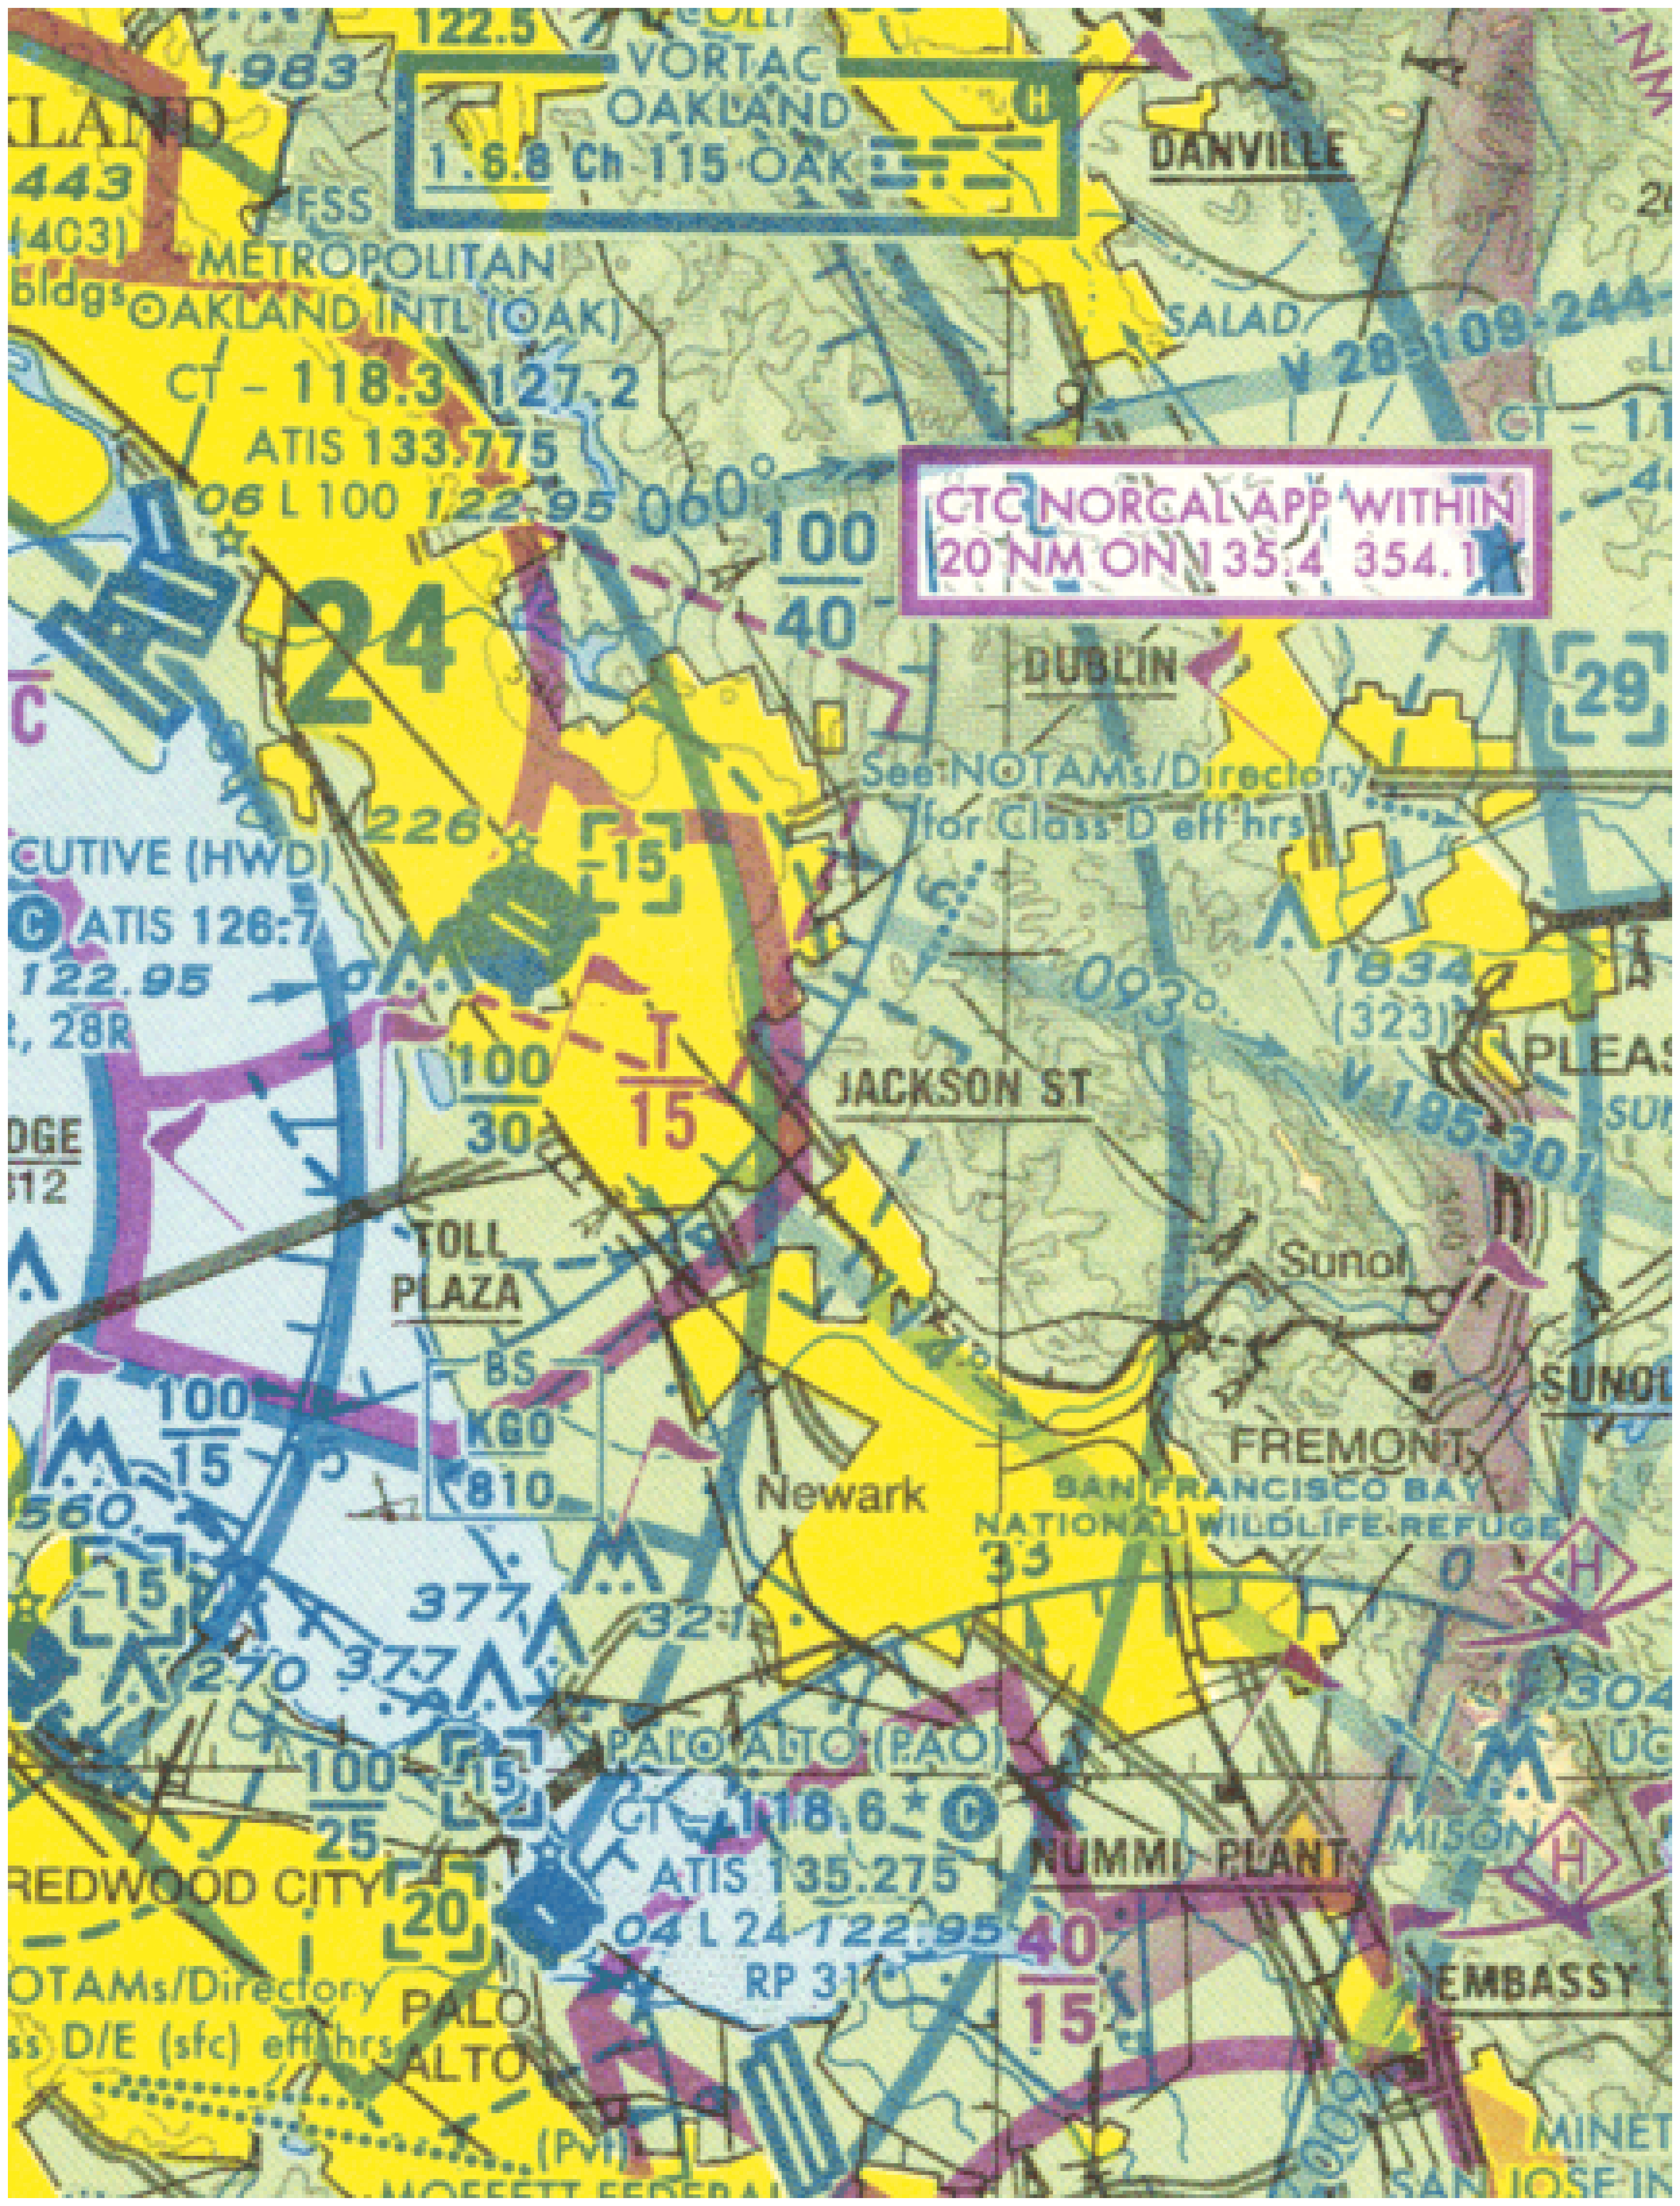
\includegraphics[width=10cm]{img/Oakland}
    \caption{Oakland VOR and 114 radial to MISON intersection}
    \label{fig:Oakland}
  \end{center}
\end{figure}

Noting our passage of that radial isn't strictly necessary --- we can
just keep flying along the 009 radial from San Jose until we need to
turn.  But it's useful for two reasons: First, it's nice to know
exactly where we are.  Second, it confirms we are where we think we
are.  If we fly and fly and never cross the radial, alarm bells should
start going off.

% 009 or 9?

Looking at the sectional, we see that the radial is the 114 radial
from the Oakland VORTAC (VOR TACAN, where TACAN stands for Tactical
Air Navigation).  Oakland's frequency is 116.8, and its ident is OAK
(\mdash\mdash\mdash\mspace \mdot\mdash\mspace \mdash\mdot\mdash).
NAV2 should already be tuned to Oakland, but if it isn't, do it
now.\marginpar{\textsf{NAV2 $\Rightarrow$ 116.8}} Turn on NAV2 in the
audio panel and make sure you're getting the correct ident.

% OAK = ---/.-/-.-

We need to adjust the OBS, to tell VOR2 which radial we're interested
in.  Set the OBS to 114\marginpar{\textsf{VOR2 OBS $\Rightarrow$
    114}}.\footnote{If you get tired of clicking on the knobs, much of
  this can be done more easily using the \textbf{\textsf{Equipment}}
  $\Rightarrow$ \textbf{\textsf{Radio Settings}} dialog.} See if you
can guess whether the flag should read TO or FROM when we cross the
114 radial.  And see if you can guess whether the needle will move
from left to right or right to left as we cross the radial.

A final note: For our purposes, there's nothing magical about the 114
radial --- we could have used 113, or 115, or 100, or 090.  The reason
I chose 114 is because there was a line on the map already drawn along
the 114 radial, which saved me the trouble of drawing a line myself.

\subsection{George II}

As we continue towards the 009 radial intercept, let's look a bit more
closely at the autopilot.  First of all, if you aren't in the habit of
trimming the airplane, you'll probably notice a flashing ``PT'' with
an arrow on the autopilot.  The autopilot is telling you to adjust the
pitch trim.  I tend to ignore it because, flying with a mouse,
trimming is more trouble than it's worth.  Those of you lucky people
with yokes and joysticks and who find flashing lights annoying might
want to trim to get rid of it.

Also, on the right there's a big knob, the altitude select knob, which
we can use to dial in a target altitude.  We're going to use it.  Turn
it until you see our desired cruising altitude, 4000 feet, displayed
on the right.  When you started turning it, ``ALT ARM'' should have
appeared in the autopilot display (as in Figure \ref{fig:ap_alt}).
This indicates that you've selected a target
altitude\marginpar{\textsf{Set autopilot altitude to 4000}}.  The
autopilot will maintain the current rate of climb until reaching that
altitude, at which point it will level off and change from vertical
speed (VS) mode to altitude hold (ALT) mode.  In altitude hold mode it
maintains an altitude (in this case our target altitude of 4000
feet).\footnote{ Of course, you don't really have to do this --- you
  could just watch the altimeter, and when it gets to 4000 feet,
  reduce the vertical speed to 0, or press the ALT button to enter
  altitude hold mode.  But by using the altitude select knob, we've
  demystified one more mystery button.}  It will also politely beep 5
times when you cross 3000 feet to remind you that you're within 1000
feet the armed altitude.

\begin{figure}
  \begin{center}
    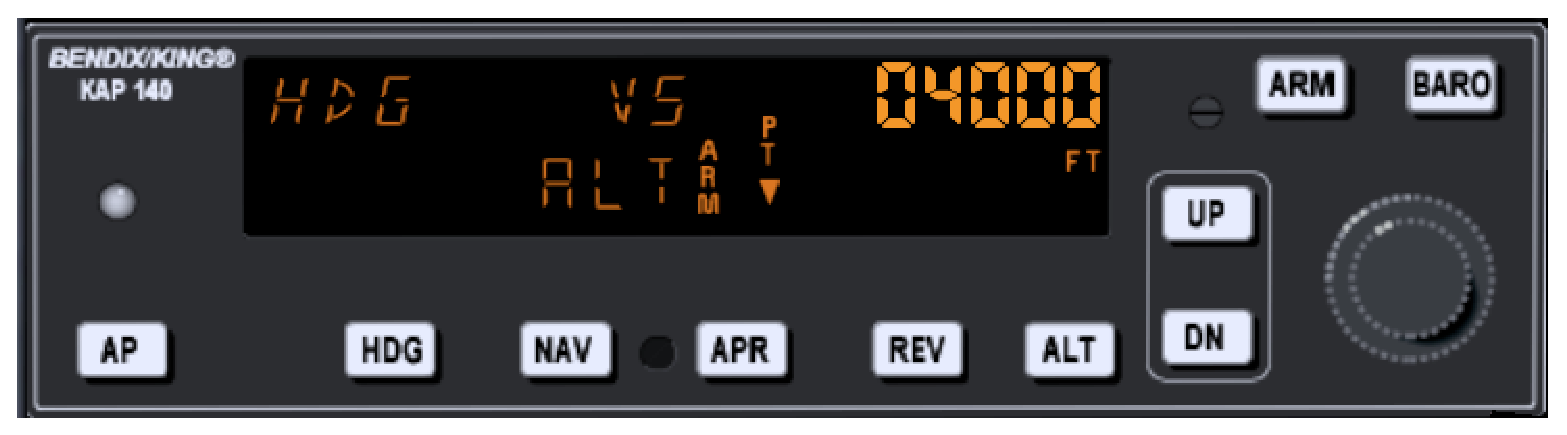
\includegraphics[width=7cm]{img/ap_alt}
    \caption{Autopilot with altitude armed}
    \label{fig:ap_alt}
  \end{center}
\end{figure}

Don't forget that the autopilot won't adjust the throttle, so when it
levels out, the airplane (and engine) will speed up.  You'll need to
adjust the throttle to get a proper cruise.

\subsection{Staying the Course}

At some point you'll intercept the 009 radial (the VOR1 needle will
centre).  Turn to a heading of 009\marginpar{\textsf{Turn to
    009$^\circ$ upon VOR1 intercept}}.  You can do this using the
heading bug on the directional gyro if you're using the autopilot.

Unless you're good or lucky, the needle probably won't be centered.
We need to adjust our course.  The CDI needle (the vertical needle on
the VOR) tells us where to go.  If it's to the left, that means the
radial is to the left, so we need to go left.  Ditto for right.

It's quite easy in theory, although in practice you may find that it's
hard to keep the needle centered, and that you are slaloming down the
radial.  The key is to realize this: the \emph{position} of the needle
tells us where we \emph{are}, the \emph{motion} of the needle tells us
what to \emph{do}.

I'll explain.  If the needle is to our left, then, yes, the radial is
definitely to our left.\footnote{Unless you're heading in the opposite
  direction, but that's another story.}  But if the needle is
\emph{moving} towards us, that means we're going to cross the radial,
sooner or later, so our situation is improving, and we probably just
need to wait for the needle to center.  On the other hand, if the
needle is \emph{moving} away, we need to turn towards it to stop, and
reverse, its motion.

Note that the amount we need to turn is difficult to guess correctly
at first, so experiment.  Try 10$^\circ$.  If the needle moves too
fast, cut it down to 5$^\circ$ (ie, turn back 5$^\circ$).  If, on the
other hand, the needle moves too slowly, double it to 20$^\circ$ (ie,
add another 10$^\circ$), and see what happens.

\subsection{Yet More Cross-Checks}

Cross-checking your position is always a good thing.  The intersection
with the Oakland 114 radial is one way\marginpar{\textsf{Cross OAK 114
    radial}}.  Ahead of that lies the SUNOL intersection.  If you look
closely, 5 separate radials join at the point, so we have an
embarrassment of choices with regards to the intersecting radial.
Because it will come in useful later, we're going to use the one
coming in from the upper right.  Another check of the sectional
reveals that this is the 229 radial of the Manteca VORTAC, 116.0 MHz,
ident ECA (\mdot\mspace \mdash\mdot\mdash\mdot\mspace \mdot\mdash).

% ECA = ./-.-./.-

You should know the drill by now: Tune NAV2 to 116.0, set the OBS to
229, and check the ident to confirm the station\marginpar{\textsf{NAV2
    $\Rightarrow$ 116.0\\VOR2 OBS $\Rightarrow$ 229}}.

Meanwhile, let's introduce another piece of gear on the panel that
will cross-check the SUNOL passage.  Some VOR stations have a distance
capability, called DME\footnote{See
  \url{http://en.wikipedia.org/wiki/Distance_Measuring_Equipment} for
  more information.} (Distance Measuring Equipment).  For example, San
Jose does (remember it's a VOR-DME station), as do Oakland and Manteca
(VORTACs have DME capabilities).

Using DME, you can find out how far you are, in straight-line
distance, from the VOR station.  In our scenario, the DME isn't
necessary, but we'll use it anyway, just to see how it works, and to
reconfirm our position.

The DME is the instrument below the autopilot (refer to Figure
\ref{fig:panel}).  Make sure it's turned on.  The selector to the left
of the on/off switch is probably set to N1, where ``N1'' means
``listen to NAV1''.  Since NAV1 is tuned to San Jose, it's telling us
the distance to the San Jose VOR-DME.  Switch the DME to
N2\marginpar{\textsf{DME $\Rightarrow$ N2}}.  It now shows us the
distance to the Manteca VOR.

The DME shows you 3 things: the distance in nautical miles to the
station, your speed towards or away from the station, and estimated
time to the station at the current speed.  Note that the distance is
the direct distance from your plane to the station (called the ``slant
distance''), not the ground distance.  Note as well that the speed is
relative to the station, so unless you're flying directly to or from
the station, it will probably be lower than your true groundspeed.
For example, the speed from San Jose, which is directly behind us,
should be greater than the speed towards Manteca, which is off to the
right.

If we look up information about the SUNOL intersection,\footnote{For
  example, from \url{http://www.airnav.com/airspace/fix/SUNOL}.} it
tells us that it is 33.35 nm (as measured by a DME receiver) from ECA
on the 229.00 radial (that's what ``ECAr229.00/33.35'' means).

Now we have two ways to confirm the SUNOL intersection: The VOR2
needle will center, and the DME will read 33.4 or so.  Note that the
DME doesn't provide us with a very precise fix here because Manteca is
at such an oblique angle.  But it does give us a good warning of
SUNOL's impending arrival.  Moreover, if it has an unexpected value
(like 30), it should raise a few alarm bells.

% EYE - acronym, then expansion, or vice-versa?

You may be wondering what ``HLD'' means (the setting between N1 and N2
on the DME).  It stands for ``hold'', and means ``retain the current
frequency, regardless of whether NAV1 or NAV2 are retuned''.  For
example, if we switch from N2 to HLD, the DME will continue to display
(and update) information to Manteca.  Even if we retune NAV2, the DME
will remain tuned to Manteca.  This is handy, because it basically
represents a third independent receiver, and in IFR flight two
receivers just never seem like enough.

\section{Getting Down}

We're getting close to SUNOL, flying along the 009 radial from San
Jose, monitoring our position with the DME.  At SUNOL we'll be less
than 5 nm from Livermore, somewhere down there in the clouds.  Perhaps
if we just descended to 700 feet or so (Livermore is at 400, the
ceiling is at 750) and headed more or less directly north after SUNOL,
we'd get there?  A recipe for disaster my friend, and you know it.

\subsection{Instrument Approach Procedures}

As you recall from the previous tutorial, when flying VFR, you don't
just point your airplane to the nearest runway to land.  You need to
fly a pattern.  This helps you line up, and helps prevent planes from
crashing into one another, which is a Good Thing.

Similarly with IFR landings.  There's a procedure to follow.  In fact,
there are \emph{procedures} to follow.  Because of the complexity of
landing in IFR conditions, there's no single procedure for all
airports.  You need to check for your particular airport.  In fact,
you usually need to check for your particular airport, runway, and
navigation equipment.

Our airport is Livermore (KLVK).  Let's check the information for that
airport.  Go to \url{http://www.airnav.com/airport/KLVK} to see what
they've got.  Down near the bottom, we have IAPs (Instrument Approach
Procedures).  There are two listed for runway 25R.  One is an ILS
(Instrument Landing System) approach, the other a GPS (Global
Positioning System) approach.  Our plane has no GPS, but it does have
ILS capabilities (I'll explain ILS later), so we'll choose that.

Although Livermore only has two different instrument approach
procedures, big airports have many many more.  If you look at nearby
San Francisco, you'll see they have a \emph{slew} of procedures.
There are ILS procedures, GPS procedures, LDA procedures, VOR
procedures, \ldots{} I wouldn't be surprised if they had a procedure
for someone with a sextant and an hourglass in there.  To learn IFR
flight, you'll need to master all of them.

Back to Livermore.  If you download the procedure, you'll see
something like Figure \ref{fig:big_plate} (except for the colour).
It's pretty overwhelming at first --- it compresses a lot of
information in a small space.  We'll ignore as much as we can,
restricting ourselves to the three parts that have been coloured in.
And we'll do those parts on a ``need to know'' basis --- we'll only
look at them when we really have to.

\begin{figure}
  \begin{center}
    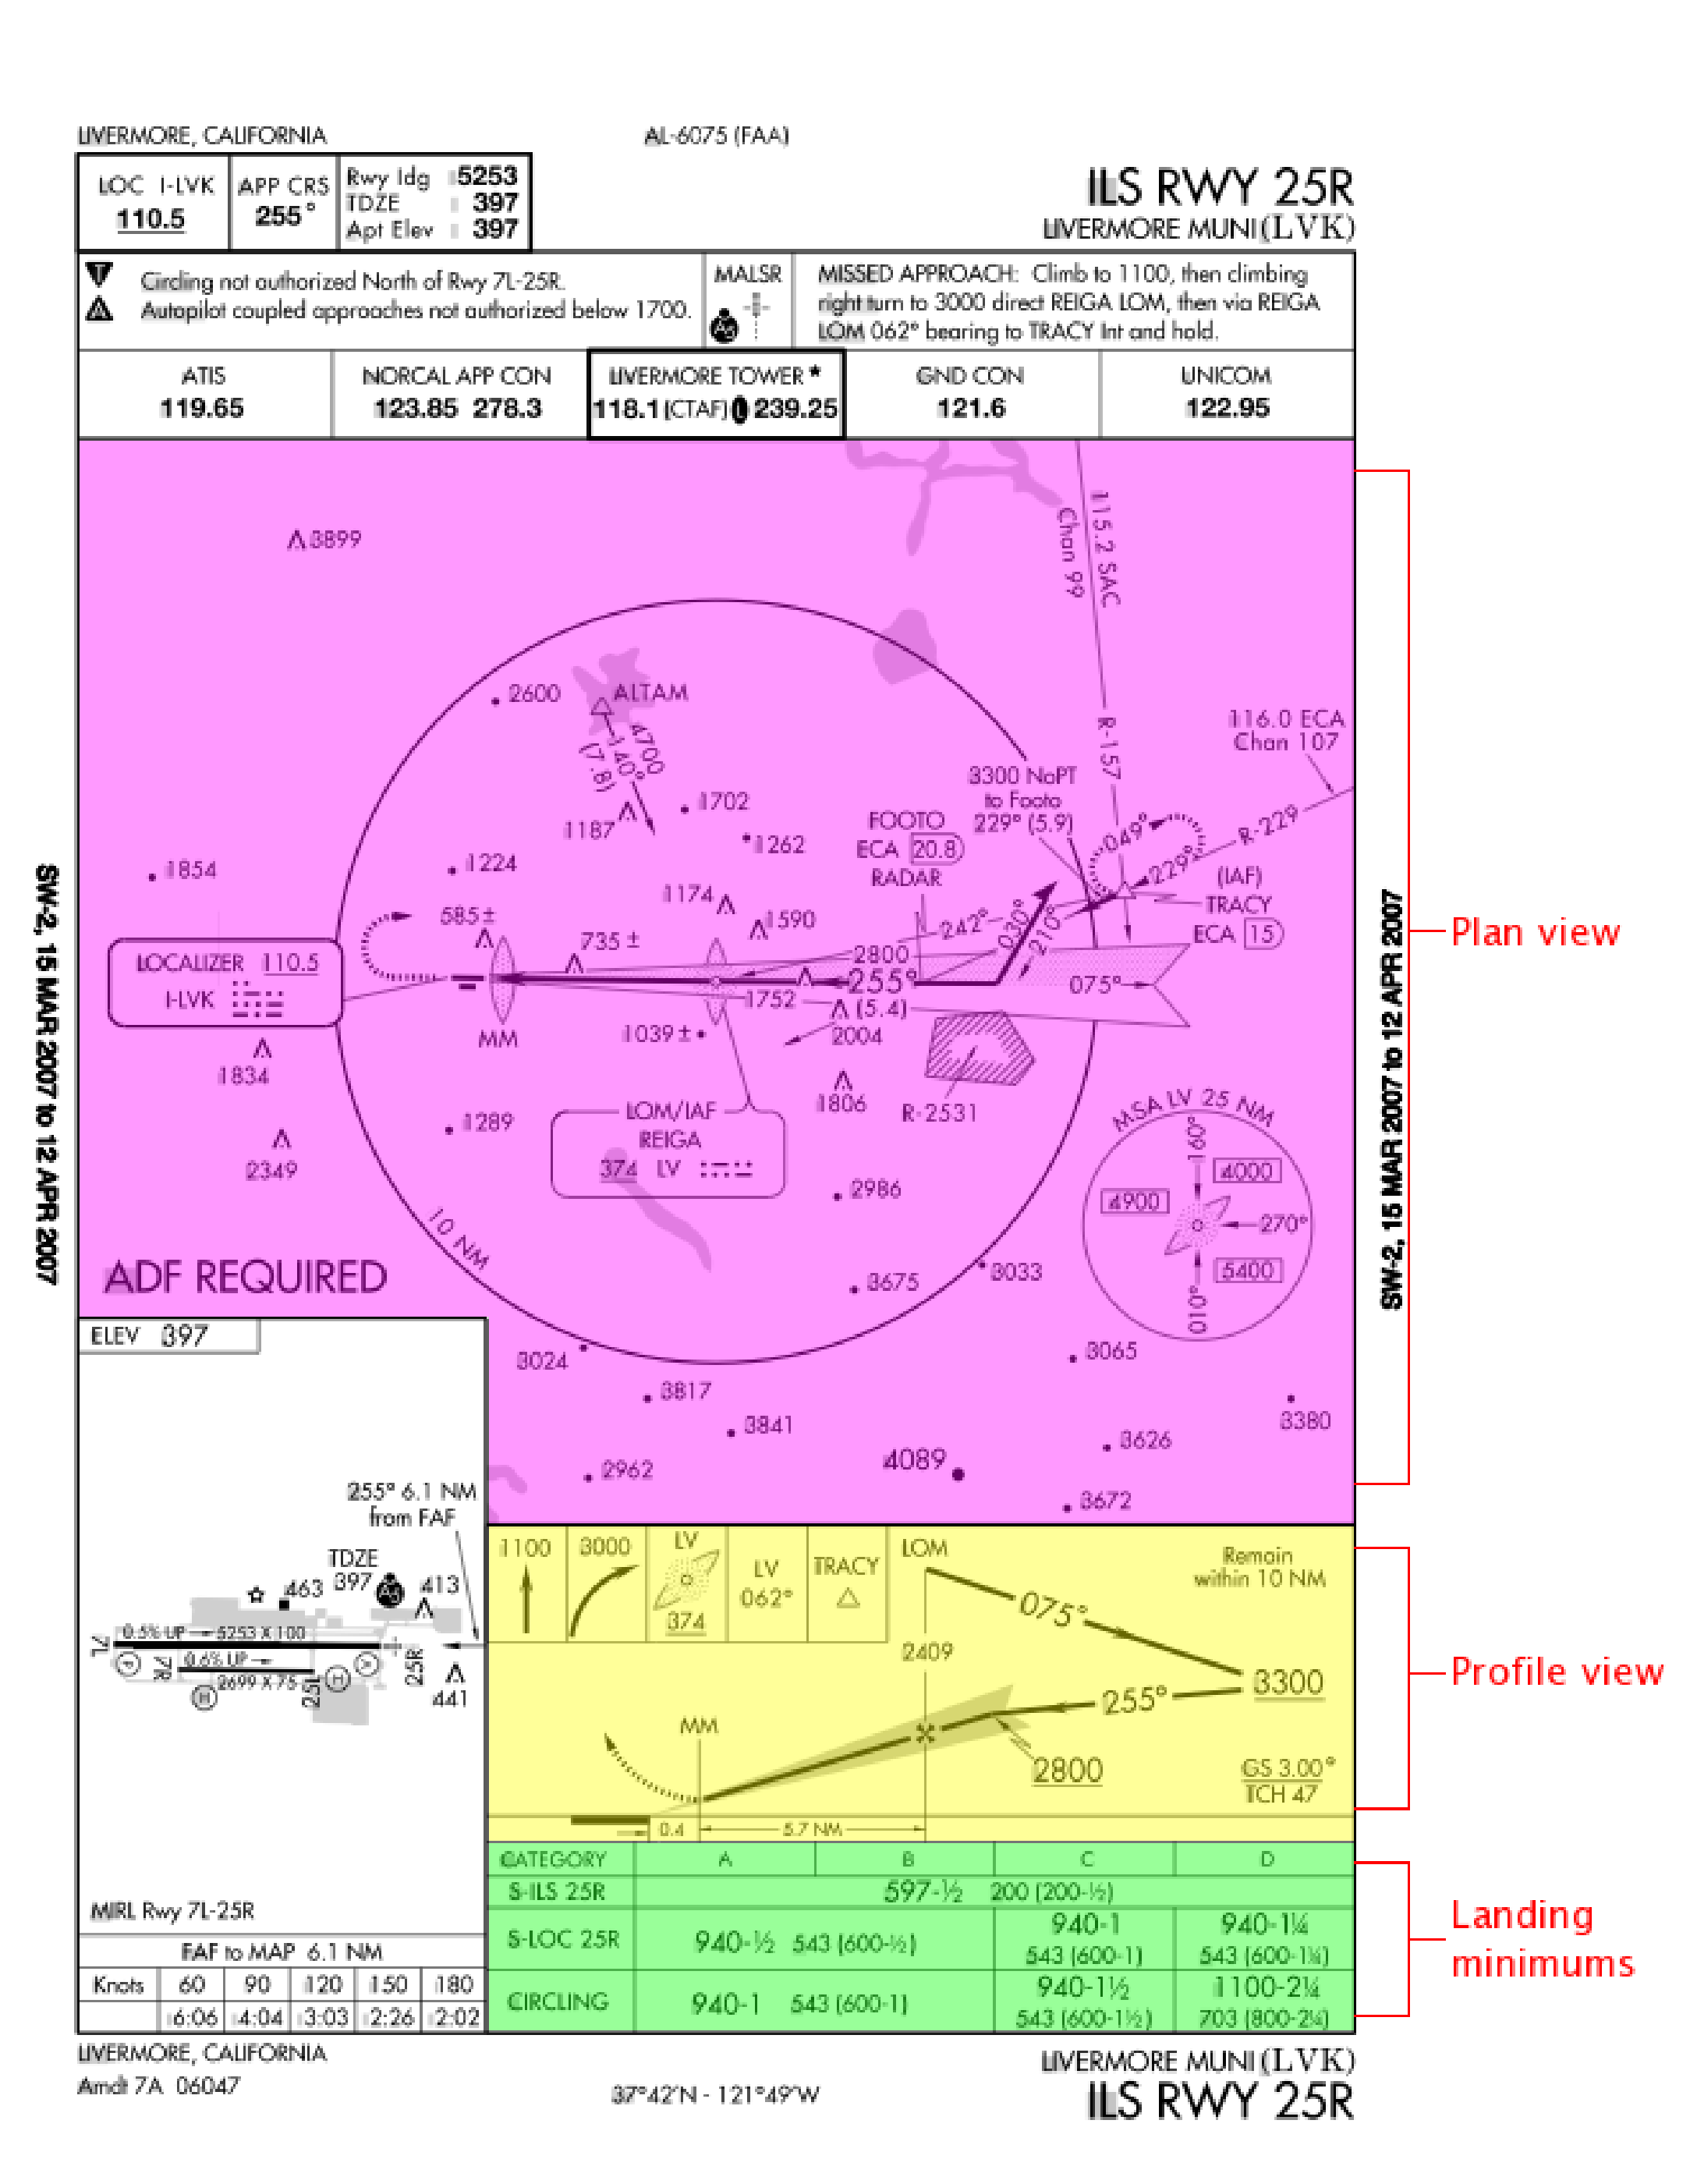
\includegraphics[width=14cm]{img/big_plate}
    \caption{ILS approach plate for Livermore runway 25R}
    \label{fig:big_plate}
  \end{center}
\end{figure}

Where to start?  At the beginning of course.  An IAP will have one or
more Initial Approach Fixes (IAFs).  These are your entry points to
the approach procedure and can be found in the ``plan view'', which
I've coloured purple in Figure \ref{fig:big_plate}.  Our IAP lists
two, one in the middle and one on the right (see Figure \ref{fig:IAFs}
for a close-up).

\begin{figure}
  \begin{center}
    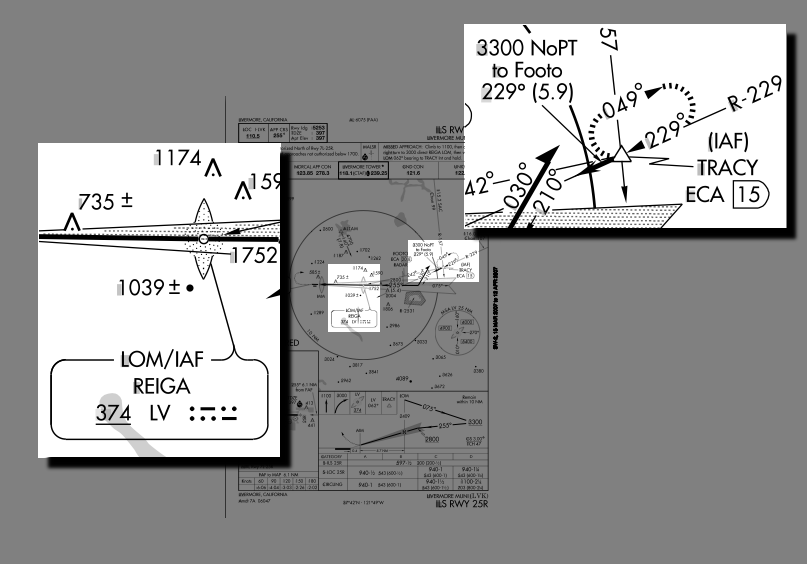
\includegraphics[width=10cm]{img/IAFs}
    \caption{Initial approach fixes}
    \label{fig:IAFs}
  \end{center}
\end{figure}

% EYE - is the altitude important?

An IAF is a \emph{fix}, and a fix is an identifiable point in space.
In fact, we've already encountered another kind of fix, namely a VOR
intersection.  Fixes are also usually named (eg, MISON, SUNOL).  The
IAF on the right is named TRACY, and consists of a radial, a distance,
and an altitude.  Specifically, it's 15 DME (15 nm as measured by a
DME receiver) along the 229 radial from the ECA (ie, Manteca) VOR.

% , at an altitude of 3300 feet.

% Notice that I said 15 DME, which means the distance in nautical
% miles as reported by a DME.  This is usually different than ground
% distance.  Notice as well we need an altitude --- the distance
% reported by the DME is straight-line distance to your plane, and so
% your height makes a difference.

\subsection{Nondirectional Beacons}

However, we're not going to use TRACY as our IAF.  We're going to use
the IAF in the middle, which is a marker (LOM stands for ``Locator
Outer Marker'').  We'll worry about what an outer marker is later.
For now let's concentrate on the locator part.  The locator in an LOM
is an NDB\footnote{See
  \url{http://en.wikipedia.org/wiki/Non-directional_beacon} for more
  information.} (Nondirectional Beacon).  It's a bit like a VOR, in
that it can be used to determine your heading and navigate from place
to place.  Like a VOR, it has a name (REIGA, in this case), a
frequency (374 kHz), and an ident (LV, or
{\mdot\mdash\mdot\mdot\mspace \mdot\mdot\mdot\mdash} in Morse).  NDBs
also appear on sectionals, as fuzzy red circles with a small circle in
the middle, with their identification information placed in a red box
nearby. (see Figure \ref{fig:NDB} for a closeup.  Don't confuse the
NDB, which is fuzzy, with the solid red circle on the left, nor the
circle below with the ``R'' inside).

% LV = .-../...-
% EYE - I checked this on one flight and it didn't sound right, and
% there were loong pauses between idents.  However, later I checked it
% from the ground at KLVK and it was fine.  Hmmm ...

\begin{figure}
  \begin{center}
    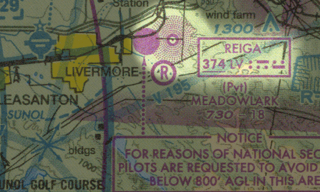
\includegraphics[width=8cm]{img/NDB}
    \caption{REIGA nondirectional beacon}
    \label{fig:NDB}
  \end{center}
\end{figure}

An NDB station basically broadcasts a signal that says ``I'm over
here'', and the receiver on the plane can receive that signal and tell
you, the pilot, ``the station is over there''.  You just need to tune
the receiver and monitor the correct instruments.  The receiver,
labelled ADF (Automatic Direction Finder) Receiver, and the
corresponding instrument, also labelled ADF, are shown in Figure
\ref{fig:panel}.

To tune into REIGA, turn the tuning knob on the receiver until 374 is
displayed as the standby (STDBY) frequency\marginpar{\textsf{ADF
    $\Rightarrow$ 374}}.  As usual, use the middle mouse button for
big changes (100 kHz in this case), and the left mouse button for
small changes (1 kHz).  Then hit the swap button (labelled ``FRQ'').
The 374 is now displayed as the selected (SEL) frequency.  The needle
on the ADF should swing around, eventually pointing ahead to the
right, to REIGA.  But it might not.  Why?  Because the receiver might
be in antenna mode (as show by the ``ANT'' in the upper-left portion
of the display).\footnote{Antenna mode, by the way, is usually used to
  ident an NDB, because it gives better audio reception.  While in
  antenna mode, however, the ADF will \emph{not} point to the station
  --- the needle will be parked pointing directly right.}  If it is in
antenna mode, hit the ADF button so that ``ADF'' shows.  Now the
needle should swing to point to REIGA.  Like VORs, to be sure we're
really tuned into the right station, we need to hear the ident as
well, so hit the ADF switch on the audio panel and check.

% EYE - ADF buttons (ADF, BFO, FRQ, FLT/ET, SET/RST)
% Aircraft/c172p/Instruments/kr87-adf/kr87.xml
% Looks like its model number is KR 87 TSO
% ADF - switches between ADF and ANT modes (who would ever use ANT?)
% BFO - beat frequency occilator (allows morse code ID to be heard on
%   unmodulated stations)
% FRQ - swaps standby and active frequencies, also shows frequencies
%   when in timer mode
% FLT/ET - swaps between flight time (since power on?) and elapsed
%   time (resetable via SET/RST).  Standby frequency is not shown.
%   Note that when the standby frequency is not shown, turning the
%   tuning knob should change the *active* frequency, but it doesn't
% SET/RST - resets the elapsed time timer (no SET as far as I can
%   tell, but the manual says you can use it to count down, so there
%   must be a way)

Notice there's no OBS to set for an ADF --- the needle just points to
the station, which is nice.  This leads us to our first rule for ADFs:

\begin{quote}
  \begin{description}
  \item[ADF Rule 1:] The needle points to the station.
  \end{description}
\end{quote}

Pretty simple.  In fact, you may not think it merits a ``rule'', but
it's important to emphasize the difference between ADFs and VORs.  A
VOR, remember, tracks a single radial, which you specify by turning
the OBS.  An ADF has a knob, and a identical-looking compass card, so
it's tempting to believe it acts the same way.  It doesn't.  Turn the
ADF heading knob (labelled ``HD'') and see what happens.  The compass
card moves, but the arrow doesn't.  It just \emph{points to the
  station}.

In our current situation, where we just want to fly to REIGA, that's
all we need to know to use the ADF.  If the needle points ``over
there'', then we'll fly ``over there'', and eventually we'll pass over
REIGA.  However, for the sake of practice, and because it will be
necessary later, I'm going to give the second rule for ADFs, which
explains what the compass card is there for:

\begin{quote}
  \begin{description}
  \item[ADF Rule 2:] \emph{If} the compass card reflects our current
    heading, then the needle gives the bearing \emph{to} the station.
  \end{description}
\end{quote}

In other words, the compass card gives ``over there'' a number.

% EYE - heading vs bearing vs track vs course
% heading: where your nose is pointed
% bearing: a radial
% tracking (v): compensating for wind to fly a constant heading and
%   bearing
% course: planned/plotted flight path
% track: actual flight path

Now we're ready to head to REIGA.  Rotate the ADF heading knob until
our current heading is at the top (basically, the ADF should match the
directional gyro).  When we pass the SUNOL intersection, look at the
ADF needle, and set the DG bug to that heading (I assume you're using
the autopilot.  If not, just turn to that heading).  At the end of the
turn, the ADF needle should point straight
ahead.\marginpar{\textsf{Cross SUNOL; turn to REIGA}} And if it
doesn't, adjust your heading so that it does.\footnote{Which is
  actually bad technique in the presence of a crosswind, but I'm
  ignoring the wind to simplify the tutorial.}

By the way, the closer you get to REIGA, the more sensitive the needle
becomes to changes in your heading.  Don't go crazy trying to keep the
needle centered as you get close.  Maintain a steady heading, and get
ready for the \ldots{}

\subsection{Procedure Turn}

So, once we hit REIGA, do we just turn left and head down to the
runway?  Ah, if only life were so simple.  No, we turn right,
\emph{away} from the airport, and do a \emph{procedure turn}.  We know
there's a procedure turn because of the barbed arrow in the plan view
(see Figure \ref{fig:PT}).  As you can see if you follow the arrow, we
need to fly away, on a heading of 075$^\circ$, then turn left
45$^\circ$ to a heading of 030$^\circ$.  We do a U-turn (to the right,
\emph{away} from the airport --- that's one of the rules about
procedure turns) to come back at 210$^\circ$, then a 45$^\circ$ right
turn to 255$^\circ$, heading straight towards the runway.  All of this
turning gives us time to set ourselves correctly on course, at the
right altitude, to land on 25R.

% EYE - get higher resolution scan?  Crop along turn?
\begin{figure}
  \begin{center}
    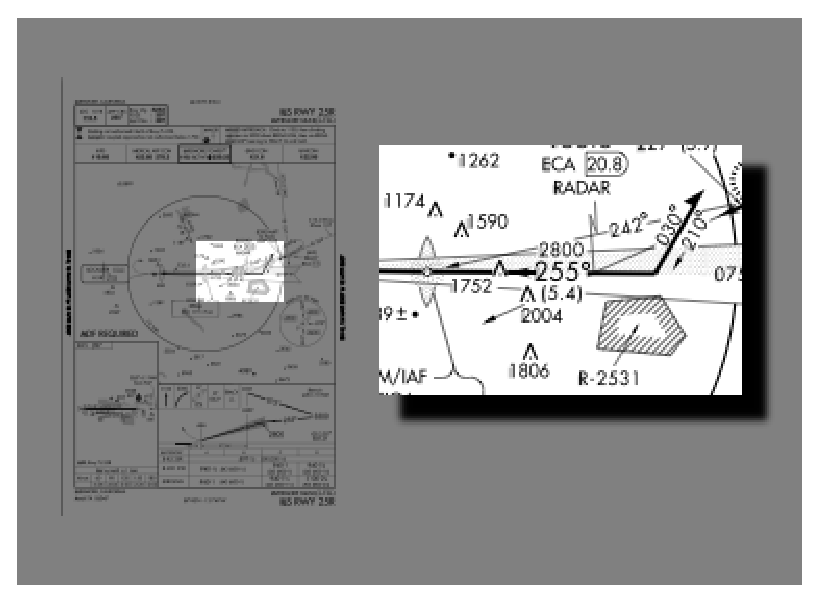
\includegraphics[width=7cm]{img/PT}
    \caption{Livermore ILS procedure turn}
    \label{fig:PT}
  \end{center}
\end{figure}

Hmmm.  I mentioned ``right altitude'', but how do we know that is?
That's down below, in the profile view (the yellow part of Figure
\ref{fig:big_plate}).  You can see that at the top is the LOM, our
IAF.  Now follow the arrows.  After the IAF, we head out at
075$^\circ$.  During the procedure turn we can descend to 3300 feet,
but \emph{no lower} (that's what the line \emph{under} the 3300
means).  After we finish our procedure turn and are heading back at
255$^\circ$, we can descend to 2800 feet, but \emph{no lower}, until
we intercept the glide slope.

One thing the instrument approach procedure does \emph{not} tell you
is the length of the procedure turn.  The only constraint is that you
must not fly more than 10 nm away from the NDB.  You'll notice there's
a 10 nm circle drawn around it in the plan view, and a note in the
profile view saying ``Remain within 10 NM''.  They're not kidding.
So, since we fly at around 110 knots, two minutes on each leg is
reasonable --- two minutes at 075$^\circ$, and two minutes at
030$^\circ$.  On the way back we don't care about times --- we just
want to intercept 255$^\circ$.

So, after we pass REIGA, turn right to 075$^\circ$.  Our ADF receiver
has a built-in timer, so we'll use that to time our two-minute leg.
Hit the ``FLT/ET'' (flight time/elapsed time) button.  The ``FRQ'' in
the middle of the display will disappear, ``FLT'' will appear on the
right, and the standby frequency will be replaced by a time.  This is
the total flight time, and cannot be changed, except by cycling the
power.  Hit ``FLT/ET'' again.  Now you'll see ``ET'' displayed, and a
time, probably the same as the flight time.  To reset the elapsed
time, hit the next switch, labelled ``SET/RST''.  The timer should
reset to 0, then start counting up (see Figure
\ref{fig:ADF}).\footnote{The timer can also be set to count down from
  a time you specify --- except that feature has not yet been
  implemented.}  In elapsed time mode, each time you hit ``SET/RST'',
the time resets to 0.  If you want to see the standby frequency again,
hit ``FRQ'' once.  The timers will continue to run.

\begin{figure}
  \begin{center}
    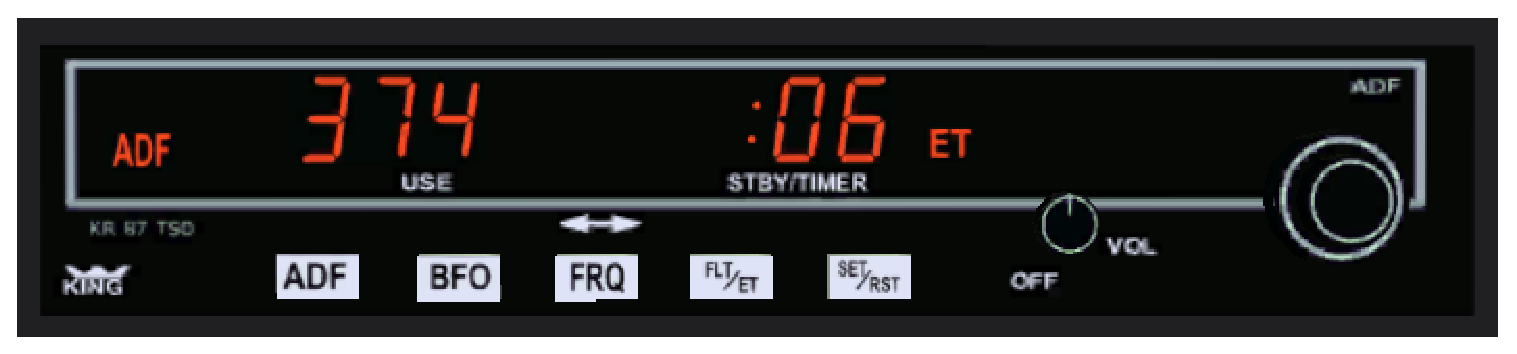
\includegraphics[width=7cm]{img/ADF}
    \caption{ADF with timer running}
    \label{fig:ADF}
  \end{center}
\end{figure}

\subsection{Chasing the Needle}

% EYE - using --ndb=LV to set my initial position doesn't work,
%       because several NDBs have the same ident
% EYE - documentation should state whether options use magnetic or
%       true headings
% EYE - do --offset-distance and --offset-azimuth only work in
%       relation to a runway specification?

% To set up FlightGear to take images of the ADF, just put it on the
% ground somewhere, and pause it.  Then, set the following two
% properties:
%
% /instrumentation/adf/rotation-deg
% /instrumentation/adf/indicated-bearing-deg
%
% to the following values:
%
% 75, 150
% 120, 115
% 120, 125
% 75, 180

When we approached REIGA, we weren't particularly concerned about our
course --- we just aimed for REIGA.  Now, however, our course is
important.  We want to be flying directly away from REIGA \emph{on a
  course of 075$^\circ$}\marginpar{\textsf{Cross REIGA; fly at
    075$^\circ$ away from REIGA for two minutes}}.

Now, in an ideal world, after we turned to 075$^\circ$, the ADF needle
would be pointed directly behind you (ie, we'd be on course).
Probably it isn't, so we need to adjust our course.  The key to
adjusting our course is ADF Rule 2.  If we've set the compass card
correctly, then the needle shows us the current NDB bearing.  If we
turn and fly until we intercept the 255 bearing, then turn to
075$^\circ$, we'll be right on course.

Figure \ref{fig:NDB_flying} shows what I mean.  In the figure, the
plane, flying along the green line, is initially off
course.\footnote{\emph{Way} off course, actually.  I've exaggerated
  the angles to make the explanation clearer.}  The heading is
correct, 075$^\circ$, but the station is at 225$^\circ$, not
255$^\circ$.  To correct this, we turn right (remembering to adjust
the ADF compass card to match our new heading).  As we fly on this new
heading, we get closer to the correct position, crossing the 235 and
245 bearings (shown in red).  Finally, when we the ADF needle points
to 255$^\circ$, we turn left to 075$^\circ$, and readjust the ADF
compass card.\footnote{You might be thinking ``Wouldn't it be nice if
  there was an ADF where the compass card rotated automatically?''
  Well, such an ADF does exist, and it comes with its own acronym ---
  RMI (Radio Magnetic Indicator).} We are now on course.

\begin{figure}
  \begin{center}
    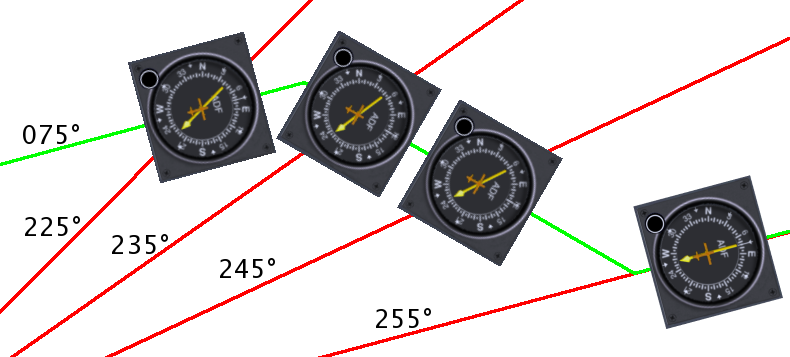
\includegraphics[width=10cm]{img/NDB_flying}
    \caption{Getting back on course}
    \label{fig:NDB_flying}
  \end{center}
\end{figure}

Of course, even when you get back on track, that won't be the end of
the story.  Your airplane drifts; your mind drifts; your compass
drifts; the wind pushes you around.  What you find is that you will be
constantly making little corrections.  That's okay, as long as we're
close.  And anyway, before long (2 minutes actually), we'll turn left
45$^\circ$ to 030$^\circ$ as part of our procedure turn, at which
point we'll just ignore the NDB anyway.  Sigh.  All that effort for
just 2 minutes.  Hardly seems worth it.

\subsection{FOOTO Time}

While you're flying outbound, take an occasional look at VOR2, tuned
to Manteca, and the DME.  Assuming the OBS is still at 229, and the
DME still tuned to N2, at some point the needle should center, meaning
you've crossed the 229 radial, and, if you're on course, at the same
time the DME should read 20.8.  How do I know that?  If you look at
the approach plate (Figure \ref{fig:big_plate}), you'll notice an
intersection, named FOOTO.  FOOTO is on the approach, and is defined
to be 20.8 DME from ECA.  Although this intersection is not strictly
necessary for us, it comes for free, and provides good confirmation of
our position both outbound and, later, inbound.

Depending on how fast you're flying, you'll probably pass FOOTO close
to the time your two minutes at 075$^\circ$ are up.  At the end of two
minutes, turn left 45$^\circ$ to 030$^\circ$.  Reset the timer, and
fly for another two minutes on this heading.

\subsection{George III}

This leg is relatively uneventful, so we'll take advantage of the lull
in the action to descend to 3300.\marginpar{\textsf{Turn left to
    030$^\circ$; fly for two minutes while descending to 3300}} Before
descending, check the KLVK ATIS (it should be 119.65 MHz) and make
sure your altimeter is correct.

Assuming you're using the autopilot, you will need to do a few things
to descend:

\begin{enumerate}
\item If you're in altitude hold (ALT) mode, you need to get back into
  vertical speed (VS) mode.  Press the ALT button --- the ``ALT'' in
  the middle of the display should change to ``VS'', and your current
  vertical speed (probably 0) should be displayed momentarily on the
  right.
\item Click the DN button until you get a vertical speed of -500 feet
  per minute.
\item If you want to set the target altitude, like before, rotate the
  big knob on the right until ``3300'' shows up on the right side of
  the display.  ``ALT ARM'' should appear on the bottom.
\end{enumerate}

Note that if you're using the autopilot to descend, it will just push
the nose down, like a bad pilot, so the airplane will speed up.  We
want to go down, but we don't want to speed up, so we need to reduce
engine RPMs to keep the speed at 110 knots.  Later, when you level off
at 3300 feet, you'll have to increase power again.

If you're flying manually, then you just need to adjust the engine to
get the descent rate you want --- the plane should stay magically at
110 knots if it's already trimmed for 110.

\subsection{ILS Landings}

While descending, we also need to start considering how we're going to
intercept 255$^\circ$ on the way back and follow it down to the
runway.  You might think we're going to use the NDB like we did on the
outbound leg, but at this point, the NDB is not good enough.  This is
an ILS landing, a so-called ``precision'' landing, and an NDB is just
not precise enough.  It can get us close to the runway, but not close
enough.

So, we're going to switch over to our ILS system.  It is much more
accurate horizontally.  As well, it offers vertical guidance,
something which the NDB does not give at all.  And hey, it also gives
you something else to learn in our few remaining minutes so that you
don't get bored.

As with NDB and VOR navigation, the ILS system\footnote{See
  \url{http://en.wikipedia.org/wiki/Instrument_Landing_System} for
  more information.} has a transmitter (or \emph{transmitters} --- a
localizer \emph{and} a glide slope) on the ground, and a receiver and
a gauge in the aircraft.  The receiver, it turns out, is just a NAV
receiver, of which we have two.  The gauge is like a VOR indicator,
but it has an added glide slope indicator, which is a horizontal (you
hope) needle.  Like a VOR, the vertical needle shows whether you're
left or right.  The horizontal needle shows whether you're high or
low.  Our ILS gauge is our old friend VOR1.

As you might have guessed, the localizer has a frequency and ident
associated with it (there's no need to tune the glide slope
separately.  If you tune the localizer, you've tuned the glide slope).
This is shown on the approach plate in two places: at the top left
corner, and in the plan view by the runway (see Figure
\ref{fig:localizer}).  As we can see, the frequency is 110.5 MHz, and
the ident is I-LVK (\mdot\mdot\mspace \mdot\mdash\mdot\mdot\mspace
\mdot\mdot\mdot\mdash\mspace \mdash\mdot\mdash).

% I-LVK = ../.-../...-/-.-

\begin{figure}
  \begin{center}
    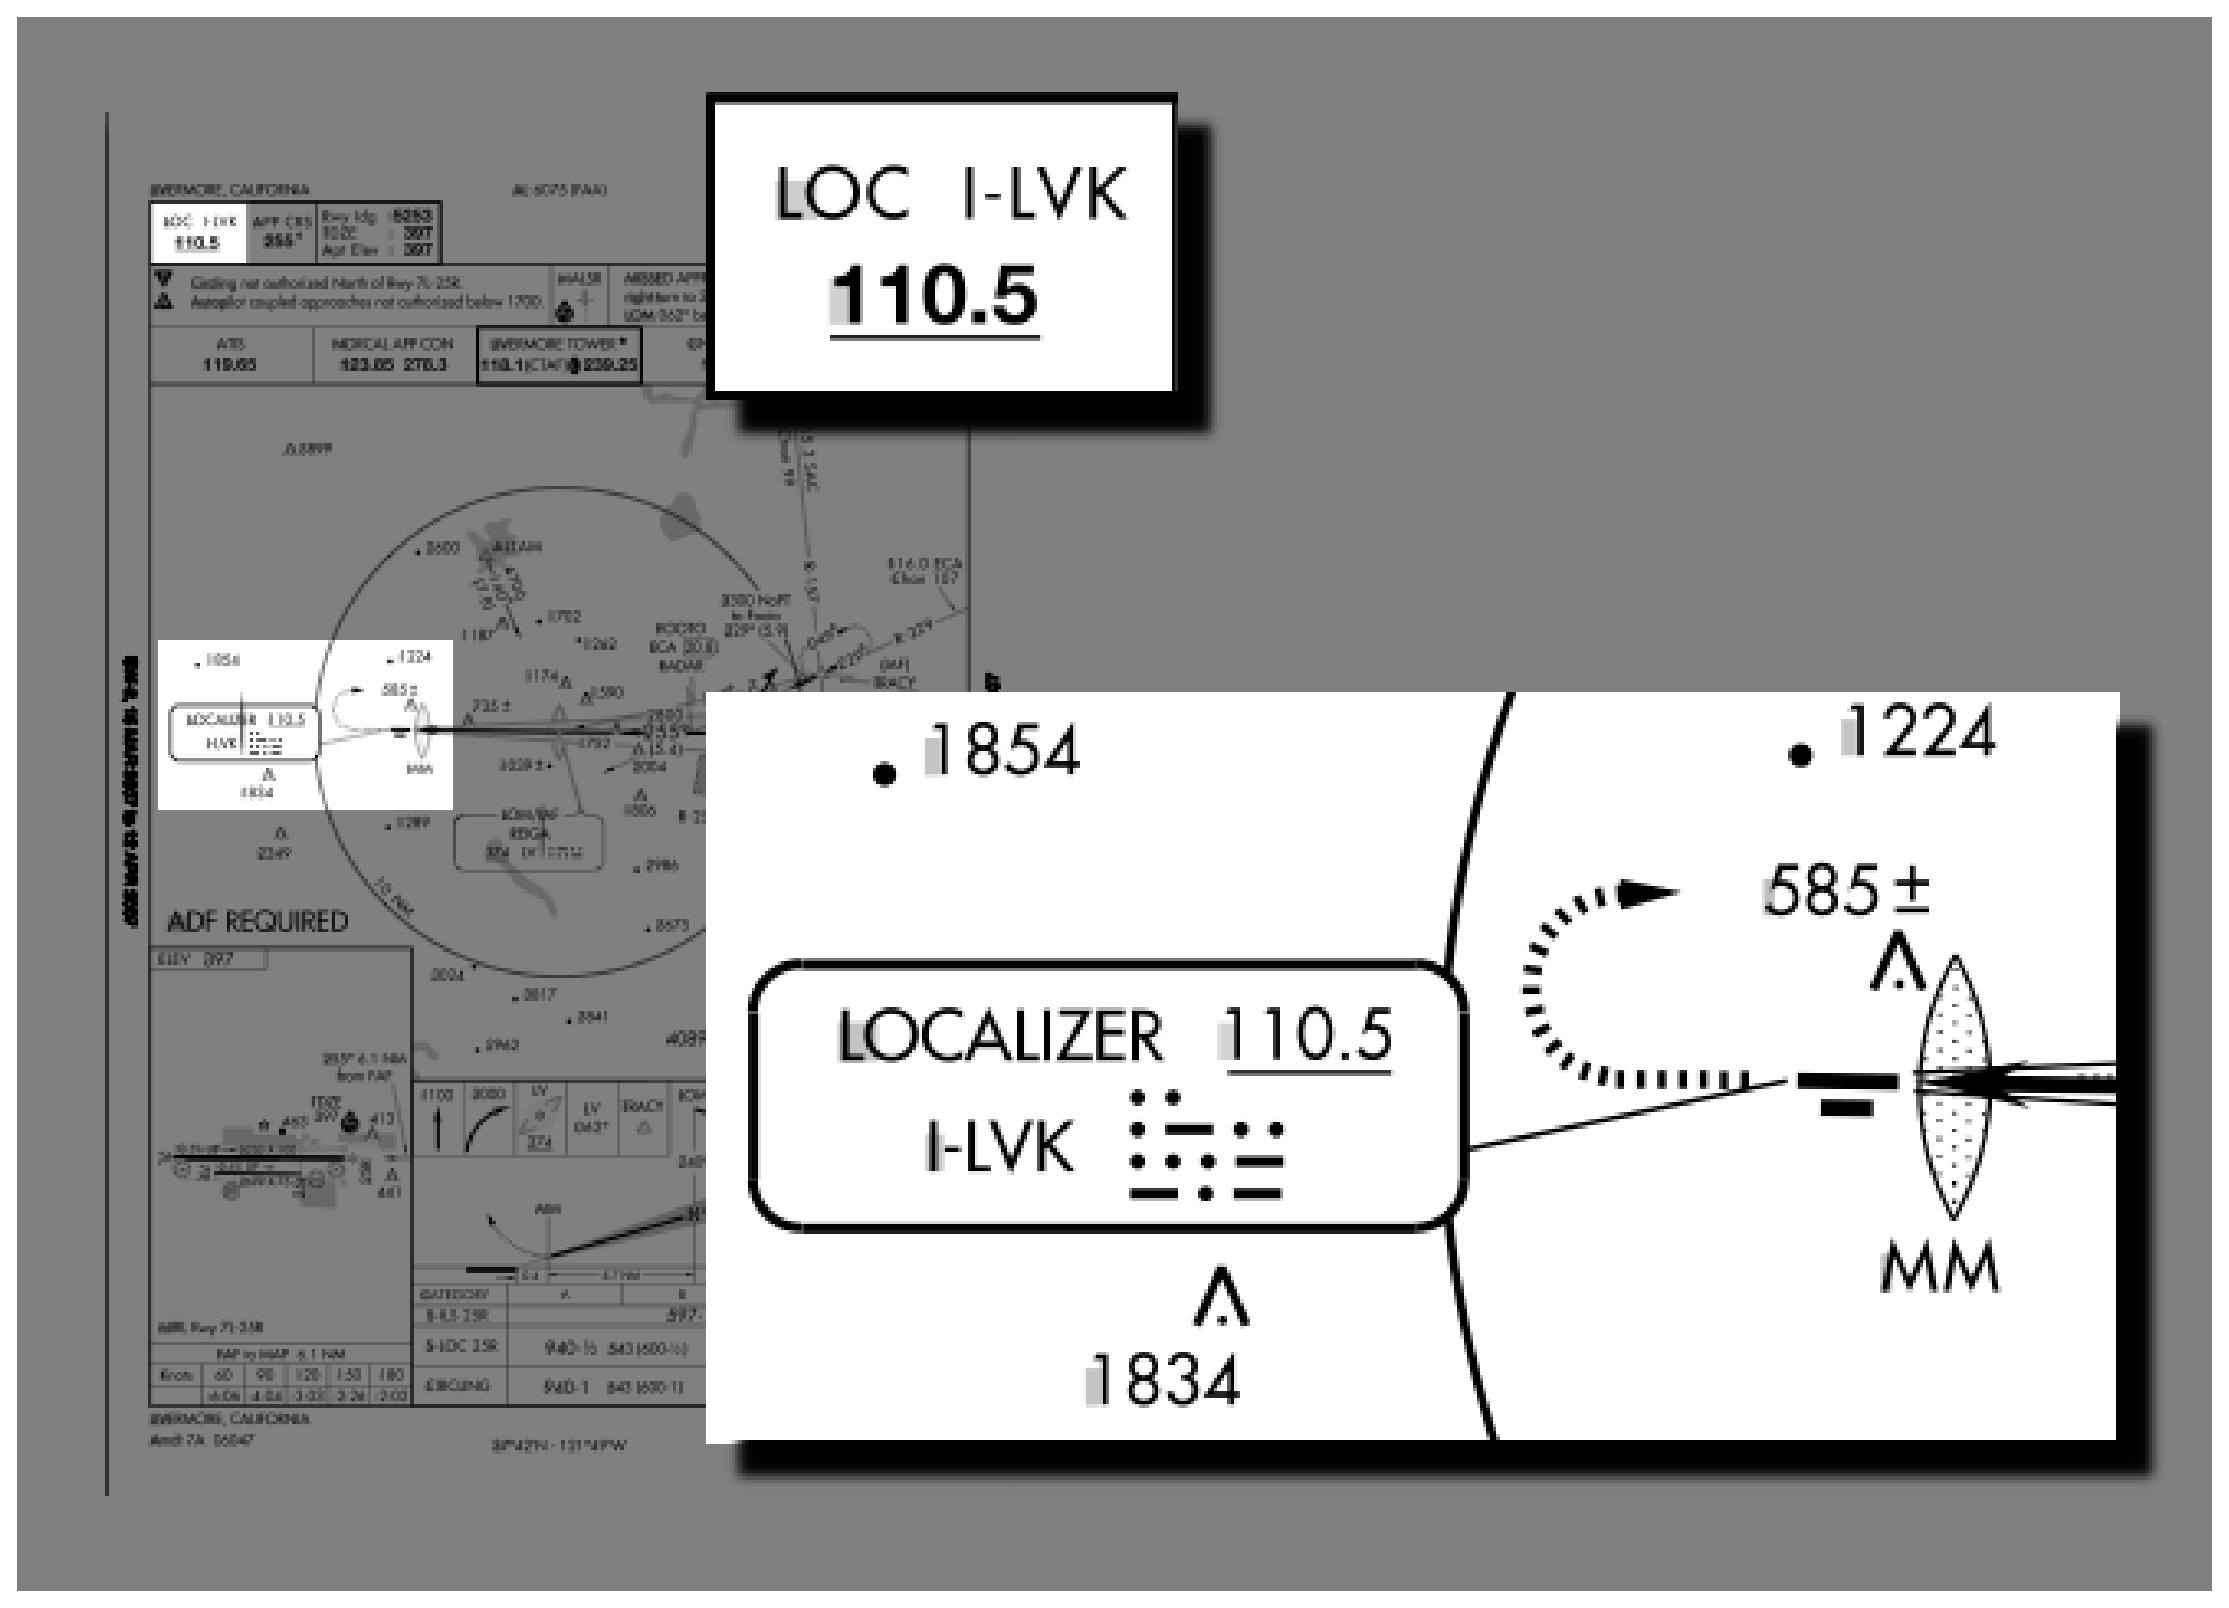
\includegraphics[width=7cm]{img/localizer}
    \caption{Livermore 25R localizer}
    \label{fig:localizer}
  \end{center}
\end{figure}

If you look at VOR1 now, it should be showing a red ``GS'' flag (this
can be seen in Figure \ref{fig:VOR1}).  This indicates that there is
no glideslope signal.  Now tune NAV1 to 110.5\marginpar{\textsf{NAV1
    $\Rightarrow$ 110.5}}.  The red ``GS'' flag should disappear.
Check for the ident.  Sounds lovely, doesn't it?  That localizer is
going to save your bacon and get you out of this interminable soup.
When you tuned into the localizer, you'll also have noticed the ILS
needles move.  And the OBS?  Well, it's useless.  Try moving it.  No
matter how you turn it, the needles don't move in response.  That's by
design.  A localizer is basically a VOR with \emph{one} radial, the
approach heading.  We don't care about any others, so we don't need an
OBS to declare interest in any others.  However, it does serve as a
useful reminder, so move the OBS to 255, our desired
heading\marginpar{\textsf{VOR1 OBS $\Rightarrow$ 255}}.

\subsection{Intercepting the Localizer}

We're now ready to intercept the ILS localizer.  When the two minutes
on the 030$^\circ$ leg have passed, make your U-turn to the right to
210$^\circ$\marginpar{\textsf{Turn right 180$^\circ$ to 210$^\circ$}}.
Soon after you complete your turn, the vertical (localizer) needle on
the ILS will begin to move.  And it will move \emph{fast}, much faster
than the ADF and VOR needles did\marginpar{\textsf{Intercept
    localizer}}.  A localizer is 4 times as sensitive as a VOR,
relatively small movements of the aircraft make big changes in the
needles.  You'll probably overshoot, but don't worry, because we have
around 5 or 10 minutes to get things straightened out.

Just remember: don't chase the needles.  That mantra is now more
important than ever.  Those needles are sensitive --- if you just turn
left when the localizer needle is to the left and right when it's to
the right, you'll be flying like a drunken sailor.  If you're lucky,
the runway will be passing underneath you as you swing across the
track for the umpteenth time.  Luck, though, is something we should
not be relying on.  Determine on how the needles are moving before
making your move.

Now that you're heading back inbound at 255$^\circ$, slow to 75 knots,
drop a notch of flaps, and descend to 2800 feet (but no
lower)\marginpar{\textsf{Slow to 75 knots; drop a notch of flaps;
    descend to 2800}}.  And check for the inbound passage of FOOTO to
confirm your position.  And pat your head and rub your stomach.

\subsection{Intercepting the Glide Slope}

As we fly towards the runway, don't forget to look at the horizontal
needle, the glide-slope needle.  When we intercepted the localizer, it
should have been high above us, because we were actually under the
glide slope.  As we levelled out at 2800, the glide slope started
coming ``down'' to us.  Eventually, you should see the needle start to
move down.  When the needle is horizontal, that means you're on the
glide slope.\footnote{Maybe.  There can be false glideslopes, and
  FlightGear models these, so we have to make sure we're on the real
  one.  One purpose of the procedure turn is to get you in the correct
  position, at the correct altitude, to intercept the true
  glideslope.}  And, soon after we intercept the glide slope, we
should pass over the outer marker.  Several things will happen more or
less simultaneously, all of which confirm your position:

% EYE - marker test (``MKR TEST'') on audio panel?

% The following site talks about airway markers:

% http://www.airwaysmuseum.com/VAR%20&%20Markers%20Ops%20Notes%201953.htm

% It seems they were used to mark positions along the old radio range
% tracks.  They could be received at altitudes of up to 20,000'.  As
% far as I know, they no longer exist.

\begin{enumerate}
\item You'll hear a continuous series of dashes.
\item The blue light labelled ``O'' above COMM1 will flash.
\item The ADF needle will swing around.
\end{enumerate}

Once on the glideslope, we need to start descending.  What's a good
rate?  It depends on our groundspeed.  In our case, we're going at 75
knots (there's almost no wind, so our airspeed and groundspeed are the
same), and it turns out that we need to descend at around 400 feet per
minute.  With the autopilot, that's pretty easy --- just dial in -400,
and you're set (but remember to reduce power to keep our speed at 75
knots, or you'll hit the runway going pretty fast, and be prepared to
adjust things if you drift above or below the glide
slope).\marginpar{\textsf{Intercept glideslope; cross outer marker;
    drop second notch of flaps}}

Without the autopilot, it's also pretty easy --- just reduce power.
How much?  In this case, with our plane, to around 1700 RPM.  Again,
it depends on many things --- plane, elevation, winds, weight,
\ldots{}, so you'll have to adjust things if you see the glide-slope
needle start to move up or down.  Like the localizer needle though,
\ldots{} (are you ready?)  DON'T CHASE IT.  Watch how it's moving,
then make your adjustment.

Since we're on final approach, you might want to drop a second notch
of flaps.  This will affect your trim, and you'll have to adjust power
a bit as well.

\subsection{Touchdown, Almost}

After all the excitement of the procedure turn, it will seem like a
long way down to the runway from the outer marker.  There's not much
to do but stare at those needles.  In fact, you'll probably stare at
them like you've never stared at them before.  Take a look around at
the other gauges too, though --- they have useful things to tell you.
Is our airspeed okay?  We don't want to stall.  RPMs about right?  If
flying manually, you'll want to constantly check the attitude
indicator and directional gyro.  This being a simulator, we don't have
to worry about oil pressure and engine temperature, but you might want
to glance over there anyway, just to get into the habit.  And I hope
you've done things like set the mixture to full rich (you did lean it
out while cruising, didn't you?).  If you want, you can lower the
flaps completely as you get closer.

\subsection{A Confession}

I've actually made you do more work than you have to.  We've been
using the autopilot as a fancy steering wheel, but it's capable of
more than that.  You may have noticed that the autopilot has some
buttons I haven't explained --- NAV, APR, and REV.  Well, using those
buttons, the autopilot can:

\begin{description}
\item[NAV:] Track a VOR radial.
\item[APR:] Do a direct ILS approach, tracking both the localizer
  \emph{and} the glideslope.
\item[REV:] Intercept the ILS before the procedure turn (ie, head
  \emph{away} from the localizer.
\end{description}

So, in fact, even more of the work you've done could have been done by
the autopilot.  After takeoff, you could have asked it to track the
009 radial from SJC all the way to SUNOL in NAV mode; at SUNOL, you
could have asked it to fly the ``back-course approach'' from I-LVK in
REV mode; done the procedure turn in HDG mode; finally, tracked the
localizer and glideslope in APR mode.

However, I didn't give you this information for two reasons.  First,
flying by hand (even with the autopilot gently holding your hand, as
we've been doing) gives you a better idea of what's happening.
Second, the autopilot doesn't behave quite as the official manual says
it should for some of these functions --- best stick to the features
that are known to work well.

\subsection{Touchdown, Not}

% EYE - a nice 1/2 symbol?

Although ILS approaches can get us close to the runway, closer than
VFR, NDB, or VOR approaches can, we still need \emph{some} visibility
to land,\footnote{Well, unless it's a Category IIIC ILS approach.} so
we need a way to decide if landing is possible or not.  That's what
the landing minimums section of the procedure plate is for (coloured
green in Figure \ref{fig:big_plate}).  In the category labelled
``S-ILS 25R'' (that's us), you'll see ``597-1/2 200(200-1/2)''.  This
tells us that we can track the glide slope down to an altitude of 597
feet (200 feet above the runway).  At 597 feet we make our decision
--- if we can't see the runway, then we have to execute a missed
approach.  597 feet is our \emph{decision height} (DH).

In addition to the altimeter, this particular approach also has
another indication that we're close --- a middle marker (MM).  This
marker will sound --- in this case, a dot dash series --- and the
yellow light labelled ``M'' above COMM1 will flash.  Passage over the
middle marker should coincide with reaching decision
height.\footnote{As you may have guessed, the remaining light ---
  white, and labelled ``A'' --- indicates passage of the inner marker.
  Our approach doesn't have one, but San Fransisco's runway 28R does.
  While passing over it, you should hear a rapid, high-pitched series
  of dots.  Why is it labelled ``A'' and not ``I''?  Because in
  ancient times, it was also used to identify passage over ``airway''
  markers along radio range tracks.}

So, what if you can't see the runway at decision height?  As you might
have expected, just as you can't land willy-nilly, you can't just go
around willy-nilly.  There's a Procedure.  A Missed Approach
Procedure.  This is shown in several places on the approach plate (see
Figure \ref{fig:MAP}): At the top, where it says ``MISSED APPROACH'',
in the plan view, where you can see a dashed arrow coming off the end
of the runway and a dashed oval on the right, and in the profile view,
where a series of boxes shows graphically what to do.  In our case,
these all tell us to:

\begin{enumerate}
\item Climb straight ahead to 1100 feet
\item Make a climbing right turn to 3000 feet
\item Fly to REIGA
\item Fly outbound from REIGA at 062$^\circ$
\item Fly a holding pattern at the TRACY intersection
\end{enumerate}

\begin{figure}
  \begin{center}
    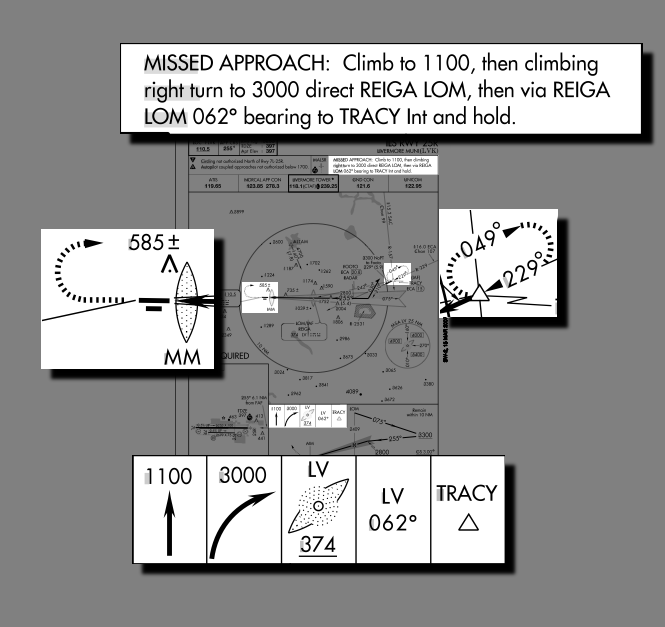
\includegraphics[width=7cm]{img/MAP}
    \caption{Missed approach procedure}
    \label{fig:MAP}
  \end{center}
\end{figure}

The holding pattern, as you might have guessed, is a place where you
can ``park'' while sorting things out, and has its own set of
procedures and techniques which we won't go into here, because
\ldots{}

\subsection{Touchdown}

In our ideal simulator world, you probably won't have to execute a
missed approach\marginpar{\textsf{Sight runway; disengage autopilot;
    cross middle marker}}.  Assuming you stayed on the glide slope,
you should have popped out of the murk at the decision height, and
with 800 metre visibility, the runway should have been in view soon
after.  With the runway in sight, you could then turn wildly to get on
course\footnote{Remembering, of course, to disengage the autopilot.}
(it's very hard to be lined up perfectly) and land ``normally'' (which
for me involves a lot of bouncing around and
cursing)\marginpar{\textsf{Land; eat hamburger}}.  Park the plane,
then stagger out of the cockpit and have another hamburger!

\begin{figure}
  \begin{center}
    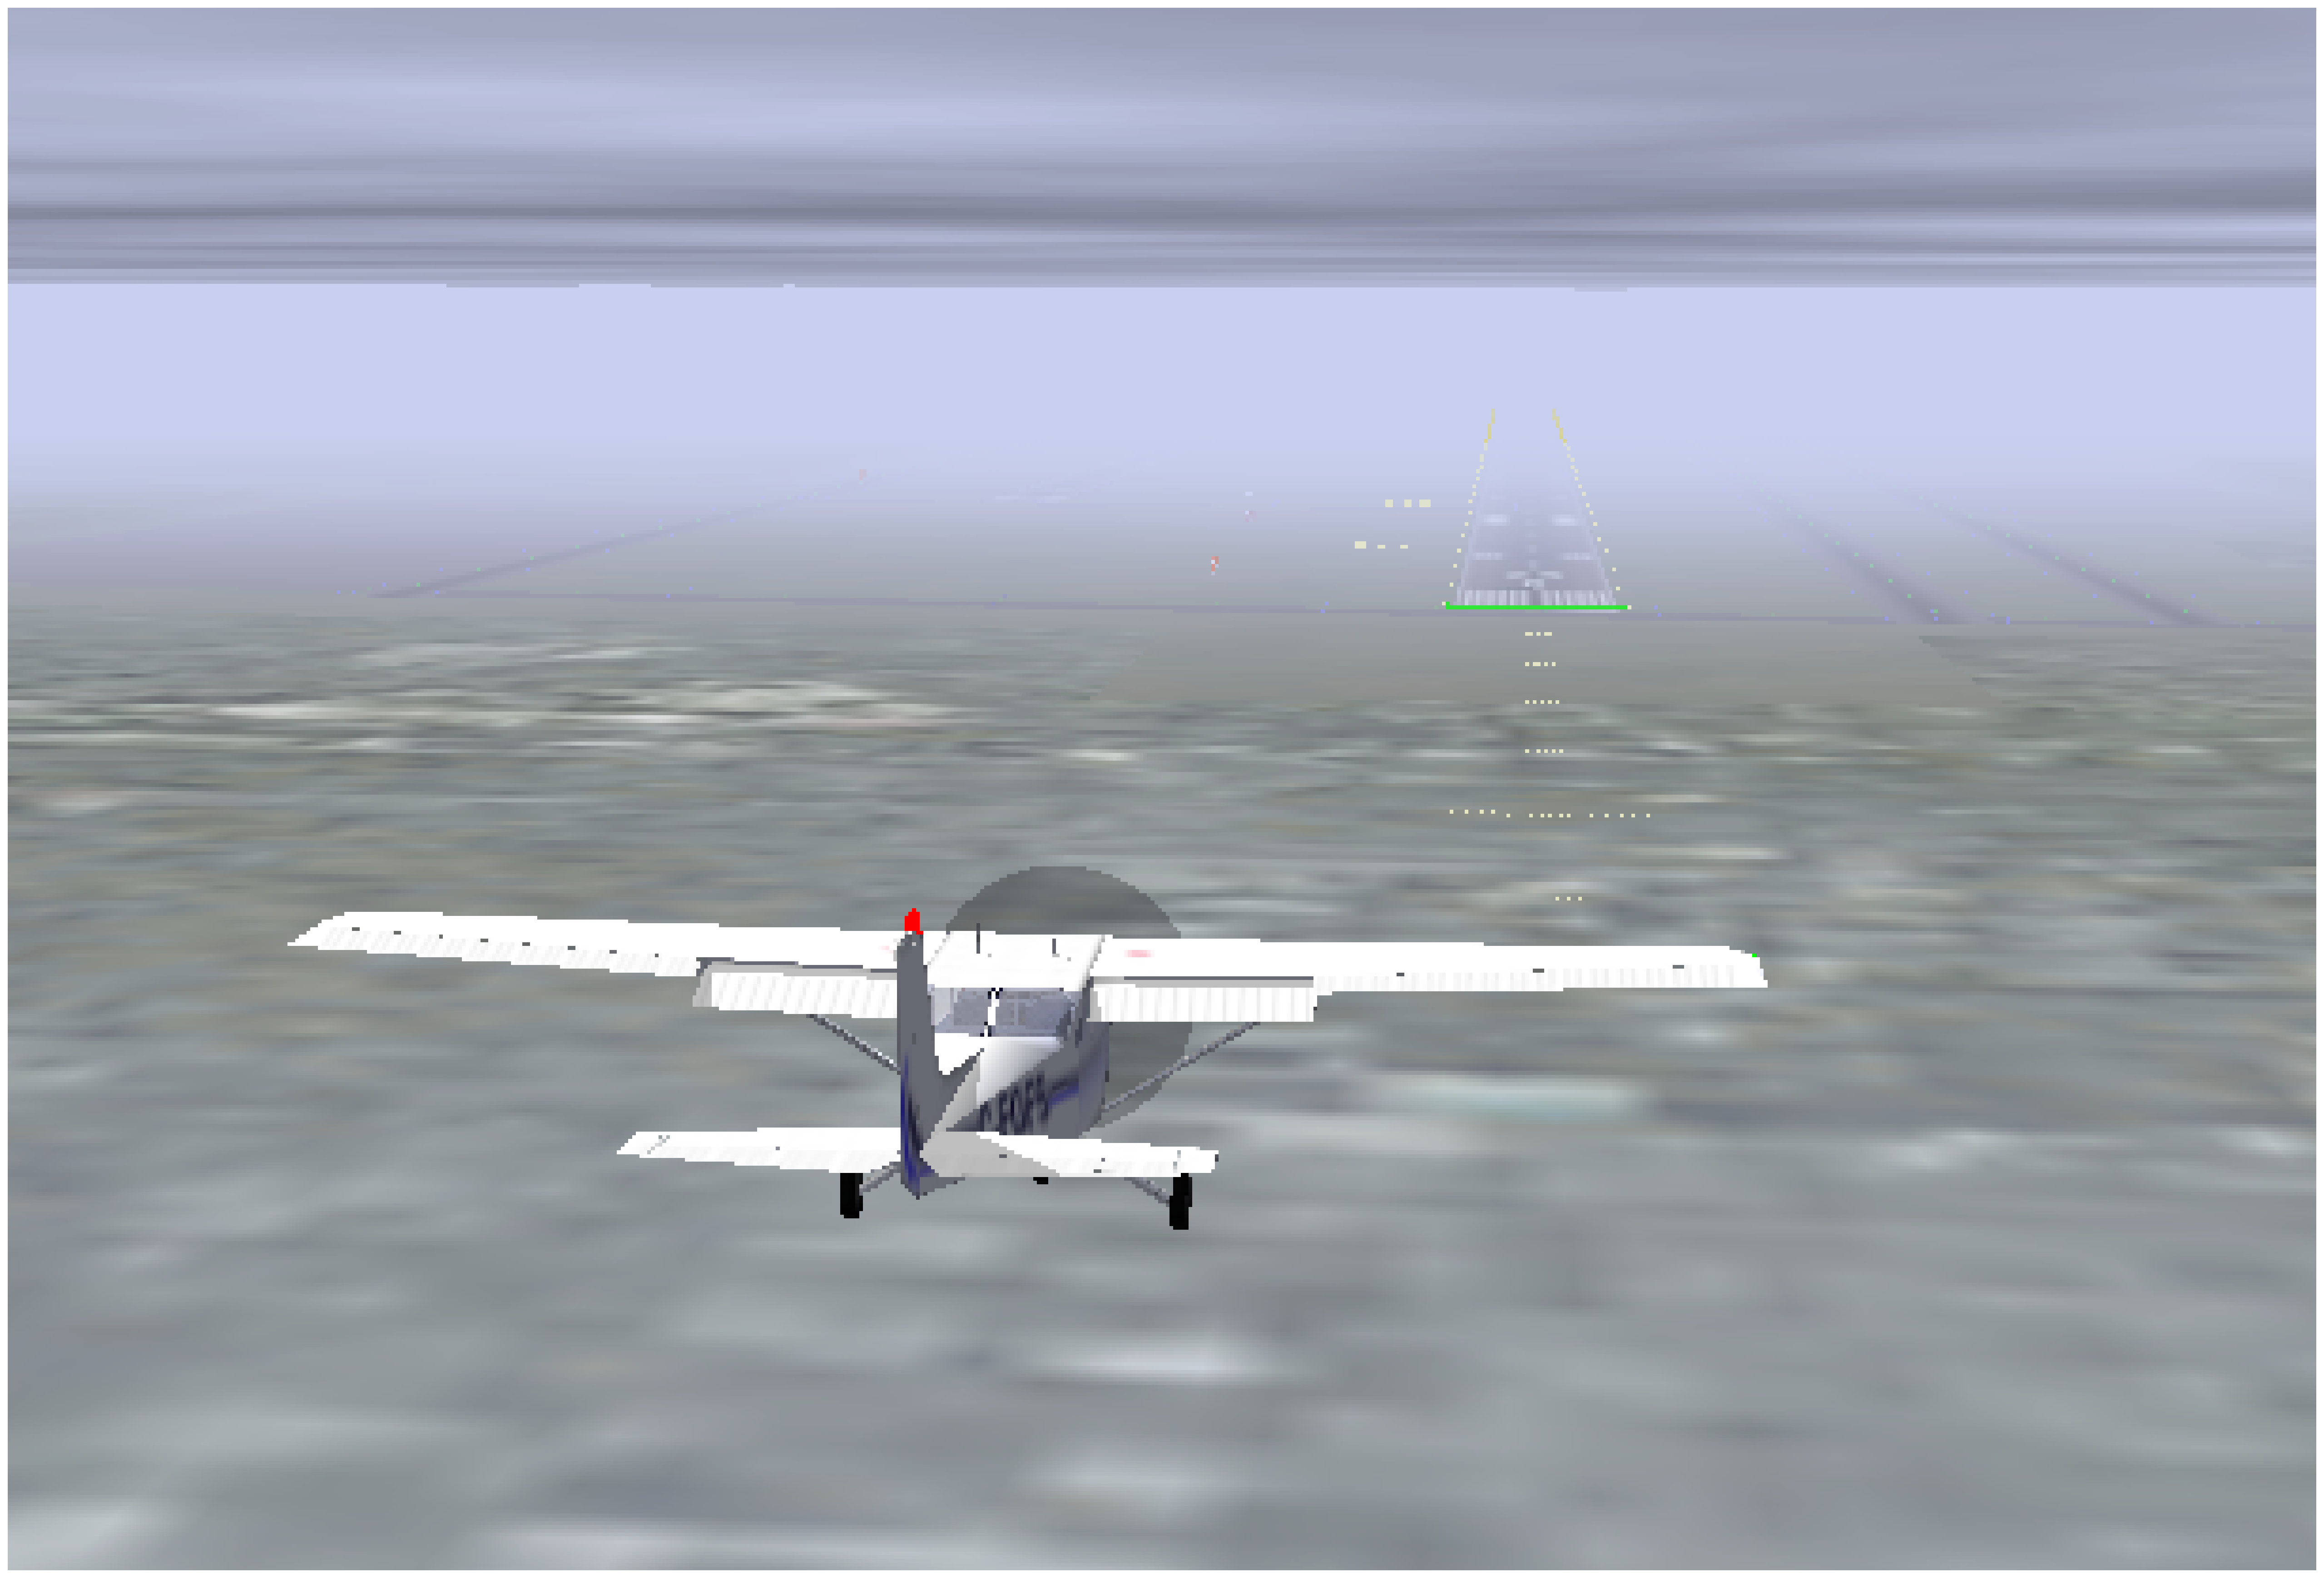
\includegraphics[width=10cm]{img/DH_plane_clipped}
    \caption{On course, runway in view.  We're going to live!}
    \label{fig:DH_plane_clipped}
  \end{center}
\end{figure}

% EYE - better navigational information websites?

\section{Epilogue}

%% There is so much more to IFR flying than what I've just presented.  In
%% FlightGear, we're all alone in our silent world and can do whatever we
%% want.  In the real world, you need to file flight plans, get them
%% approved, watch out for traffic, stay in contact with ATC, accept
%% instructions (which may deviate from your oh-so-carefully-conceived
%% flight plan), \ldots{}, the list goes on and on.  As if flying wasn't
%% hard enough, with ATC you need to fly and talk at the same time!

That was a lot of information in a short time, a rather brutal
introduction to ILS flying.  Hopefully, instead of turning you off, it
has whetted your appetite for more, because there \emph{is} more.
Some of the major issues I've ignored are:

\begin{description}
\item[Wind] This is a big one.  Flying IFR in a crosswind affects
  everything you do, and you need to be aware of it or your navigation
  will suffer.
\item[Flying without the autopilot] George tries his best, but he's
  not completely trustworthy.  You have to be prepared to go it
  alone.
\item[DG precession] The directional gyro in the c172p is not perfect.
  Over time, the values it gives you are less and less reliable --- it
  \emph{precesses}.  It needs to be periodically calibrated against
  the compass (using the OBS knob on the DG to adjust it).
\item[IFR charts] We used sectionals, which are really intended for
  VFR flight.  There are a whole set of charts devoted exclusively to
  IFR flight.
\item[ATC] The other people out there need to know what you're doing.
  As well, they'll probably tell you what to do, including to ignore
  the approach plate you so fastidiously studied.
\item[SIDs/DPs, Airways, and STARs] This tutorial introduced IAPs,
  which are standard ways to make approaches.  In IFR flight, there
  are standard ways to \emph{leave} airports (Standard Instrument
  Departures, \emph{SIDs}, or Departure Procedures, \emph{DPs}),
  standard ways to travel \emph{between} airports (airways), and
  standard ways to go from airways to IAPs (Standard Terminal Arrival
  Routes, \emph{STARs}).
\item[Holding Patterns] Most missed approaches end in a holding
  pattern somewhere, so you'd better know how to fly them.
\item[GPS] Our Cessna doesn't have a GPS, but nowadays most small
  planes do, and GPS is rapidly replacing radio-based navaids.
\end{description}

If you want to learn more, try the following resources:

\begin{itemize}
\item \href{http://www.navfltsm.addr.com}{\textit{Flight Simulator
    Navigation}}, written by Charles Wood.  It covers everything from
  basic navigation to ILS approaches, with lots of examples and
  practice flights to improve your skills.  Everything is linked
  together by an entertaining storyline in which you are the pilot for
  a fictional charter service.

  Two caveats, though.  First, it is Microsoft Flight Simulator-based,
  so you'll have to translate into ``FlightGear-ese'' as appropriate.
  Second, it is a bit out of date, and things in the real world have
  changed since it was written.  NDB beacons have been decommissioned,
  new approaches have replaced old ones --- even an airport has
  disappeared (!).  Treat this as a learning opportunity.  You'll get
  better at finding more up to date information, and learn not to
  blindly trust your charts, just as you have learned not to blindly
  trust your instruments.

\item If you're \emph{really} keen and want to hear it straight from
  the horse's mouth, there's the official
  \href{http://www.faa.gov/regulations_policies/handbooks_manuals/aviation/media/FAA-H-8083-15B.pdf}{\textit{FAA
      Instrument Flying Handbook}}.  It's big and detailed, and
  there's \emph{no} interesting storyline in which you're a pilot for
  a fictional charter service.  More documents can be found at their
  \href{http://www.faa.gov/regulations_policies/handbooks_manuals/aviation/}{\textit{Aviation
      Handbooks \& Manuals}} page.

% http://www.faa.gov/regulations_policies/handbooks_manuals/aviation/

\item If you'd like practice deciphering what the instruments are
  telling you, without the bother flying (or even virtual flying), you
  can try
  \href{http://www.luizmonteiro.com/Learning.aspx}{\textit{luizmonteiro.com}},
  which has Flash tutorials of various instruments, including a VOR
  and an ADF.

\item Another simulated instrument site is
  \href{http://www.visi.com/~mim/nav/}{\textit{Tim's Air Navigation
      Simulator}}.  It has a Java applet that simulates a plane flying
  in the vicinity of two navaids.  The simulation allows you to use
  different kinds of instruments and navaids, so you can see their
  behaviour, and the advantages and disadvantages of each.

\item If it's navigation information you're after, an excellent site
  is \href{http://www.airnav.com}{\textit{AirNav.Com}}, which I've
  used extensively in the course of this tutorial.  It has detailed
  airport, navaid, and fix information, and links to IAPs.
  Unfortunately, the information is only for the USA.

\item Another source of airport and navaid information is
  \href{http://worldaerodata.com}{\textit{World Aero Data}}.  Its
  information isn't as detailed as AirNav's, but it is international.

\item \textit{FlightSim.Com} has a very informative series of articles
  entitled
  \href{http://www.flightsim.com/vbfs/content.php?2133}{``How
    To \ldots{} Use Approach Plates''}.  It starts with a \emph{very,
    very} dense tutorial on how to read an approach plate, then
  follows with a set of approaches at Kodiak, Alaska.  These are an
  excellent supplement to the approaches given in Charles Wood's
  \textit{Flight Simulator Navigation} (see above).

  Most interesting, though, is section two --- ``Dangerous
  Approaches.''  Approaches at six airports around the world, from
  Penticton, BC to Kathmandu, Nepal, are described.  Fly them if you
  dare!

  Warning --- the series is even more Microsoft Flight
  Simulator-centric than Charles Wood's, and some of it is out of date
  (some outside links are broken, and some of the approaches have
  changed).

% Add?
%
% http://www.acukwik.com/
%
% More airport and flying information

% Add?
%
% http://www.fsstation.com/tutorials/approachplates.html
%
% Another short tutorial on approach plates.

% Add?
%
% http://www.fsstation.com/tutorials/dangerous-airports-approaches.html
%
% Five approaches with short descriptions.

% Add?
%
% http://www.flightsim.com/cgi/kds?$=main/howto/glass/glass.htm
%
% An explanation of glass cockpits.  It's pretty good, but still
% leaves a fair bit unexplained.

% Add?
%
% http://www.fsstation.com/tutorials/boeing-pmdg-737ng.html
%
% A complete flight in a nice 737 simulation.  Has descriptions of
% using the Flight Management Computer (FMC), and many pictures of the
% Primary Flight Display (PFD) and Navigation Display (ND).  Often it
% talks about the ``FMA'' (Flight Mode Annunciator), which are the
% labels at the top of the PFD.

% Add?
%
% http://www.united-virtual.com/classes/index.html
%
% The first entry in a series about flying with another virtual
% airline (United, in this case).  It's geared totally toward big
% airliners, so offers a different perspective on things.  It's a nice
% introduction, providing useful information without expecting you to
% know everything already.

% Add?
%
% http://www.jeppesen.com/wlcs/index.jsp?section=resources&content=publications_aopa.jsp
%
% A page with pointers to 3 sets of publications: 'Jeppesen Electron
% Chart Clinic, 'The NavData Chart Clinic', and 'The Chart Clinic'.
% It's all Jeppesen specific of course, but the 'Chart Clinic' series
% looks like it may be generally useful.

% Add?
%
% http://www.free-online-private-pilot-ground-school.com/index.html
%
% As the URL indicates, a free, online, private pilot ground school.

\item Also from \textit{FlightSim.Com} is
  \href{http://www.flightsim.com/vbfs/content.php?1756}{``Golden
    Argosy''}, a description of a flight from New York to Rome by Tony
  Vallillo, an American Airlines 767 captain.  It gives some
  interesting information about navigation that doesn't appear in the
  other sites mentioned here, such as the North Atlantic Tracks.
  However, its main appeal is that it gives a good answer to the
  question ``What's it \emph{really} like to be a pilot?''  The
  author's love of flying is evident throughout the article.

\item For those who are interested in the ATC side of things, and want
  information from an authoritative source, check out Michael Oxner's
  \href{http://bathursted.ccnb.nb.ca/vatcan/fir/moncton/WeeklyTopics/WeeklyTopicIntro.html}{``Aviation
    Topic of the Week''}, a series of articles about flying ``in many
  types of airspaces in many situations.''  Michael Oxner is a
  professional controller and private pilot who obviously can't get
  enough of airplanes, because in his spare time he's also an on-line
  controller with VatSim.  Particularly interesting are a set of
  articles describing a complete IFR flight and a complete VFR flight.

%% \item Holds are mentioned frequently, but rarely described (viz., this
%%   tutorial).  A good description can be found at:

%%   \url{http://www.flightsim.com/cgi/kds?$=main/howto/hold2.htm}

%% \item Freeworld Airways is a virtual airline.  Their
%%   \href{http://www.freeworld-airways.net/main/training.php}{``flight
%%     school''} has lots of useful information about navigation
%%   (including holding patterns, SIDs, and STARs), ATC and
%%   communication, and weather.

%%   Also interesting are two example flights, one in Europe and one in
%%   North America, showing the interaction between pilot and ATC.

\end{itemize}
\fi
